<<<<<<< 748b67fd60b26d45750e10209255345ebe612814
\documentclass[
  bibliography=totoc,     % Literatur im Inhaltsverzeichnis
  captions=tableheading,  % Tabellenüberschriften
  titlepage=firstiscover, % Titelseite ist Deckblatt
]{scrartcl}

% Paket float verbessern
\usepackage{scrhack}

% Warnung, falls nochmal kompiliert werden muss
\usepackage[aux]{rerunfilecheck}

% unverzichtbare Mathe-Befehle
\usepackage{amsmath}
% viele Mathe-Symbole
\usepackage{amssymb}
% Erweiterungen für amsmath
\usepackage{mathtools}

% Fonteinstellungen
\usepackage{fontspec}
% Latin Modern Fonts werden automatisch geladen
% Alternativ zum Beispiel:
%\setromanfont{Libertinus Serif}
%\setsansfont{Libertinus Sans}
%\setmonofont{Libertinus Mono}

% Wenn man andere Schriftarten gesetzt hat,
% sollte man das Seiten-Layout neu berechnen lassen
\recalctypearea{}

% deutsche Spracheinstellungen
\usepackage{polyglossia}
\setmainlanguage{german}


\usepackage[
  math-style=ISO,    % ┐
  bold-style=ISO,    % │
  sans-style=italic, % │ ISO-Standard folgen
  nabla=upright,     % │
  partial=upright,   % ┘
  warnings-off={           % ┐
    mathtools-colon,       % │ unnötige Warnungen ausschalten
    mathtools-overbracket, % │
  },                       % ┘
]{unicode-math}

% traditionelle Fonts für Mathematik
\setmathfont{Latin Modern Math}
% Alternativ zum Beispiel:
%\setmathfont{Libertinus Math}

\setmathfont{XITS Math}[range={scr, bfscr}]
\setmathfont{XITS Math}[range={cal, bfcal}, StylisticSet=1]

% Zahlen und Einheiten
\usepackage[
  locale=DE,                   % deutsche Einstellungen
  separate-uncertainty=true,   % immer Fehler mit \pm
  per-mode=symbol-or-fraction, % / in inline math, fraction in display math
]{siunitx}

% chemische Formeln
\usepackage[
  version=4,
  math-greek=default, % ┐ mit unicode-math zusammenarbeiten
  text-greek=default, % ┘
]{mhchem}

% richtige Anführungszeichen
\usepackage[autostyle]{csquotes}

% schöne Brüche im Text
\usepackage{xfrac}

% Standardplatzierung für Floats einstellen
\usepackage{float}
\floatplacement{figure}{htbp}
\floatplacement{table}{htbp}

% Floats innerhalb einer Section halten
\usepackage[
  section, % Floats innerhalb der Section halten
  below,   % unterhalb der Section aber auf der selben Seite ist ok
]{placeins}

% Seite drehen für breite Tabellen: landscape Umgebung
\usepackage{pdflscape}

% Captions schöner machen.
\usepackage[
  labelfont=bf,        % Tabelle x: Abbildung y: ist jetzt fett
  font=small,          % Schrift etwas kleiner als Dokument
  width=0.9\textwidth, % maximale Breite einer Caption schmaler
]{caption}
% subfigure, subtable, subref
\usepackage{subcaption}

% Grafiken können eingebunden werden
\usepackage{graphicx}
% größere Variation von Dateinamen möglich
\usepackage{grffile}

% schöne Tabellen
\usepackage{booktabs}

% Verbesserungen am Schriftbild
\usepackage{microtype}

% Literaturverzeichnis
\usepackage[
  backend=biber,
]{biblatex}
% Quellendatenbank
\addbibresource{lit.bib}
\addbibresource{programme.bib}

% Hyperlinks im Dokument
\usepackage[
  unicode,        % Unicode in PDF-Attributen erlauben
  pdfusetitle,    % Titel, Autoren und Datum als PDF-Attribute
  pdfcreator={},  % ┐ PDF-Attribute säubern
  pdfproducer={}, % ┘
]{hyperref}
% erweiterte Bookmarks im PDF
\usepackage{bookmark}

% Trennung von Wörtern mit Strichen
\usepackage[shortcuts]{extdash}

\author{%
  AUTOR A\\%
  \href{mailto:authorA@udo.edu}{authorA@udo.edu}%
  \texorpdfstring{\and}{,}%
  AUTOR B\\%
  \href{mailto:authorB@udo.edu}{authorB@udo.edu}%
}
\publishers{TU Dortmund – Fakultät Physik}


\subject{Versuch 351}
\title{Fourier- Analyse und Sythese}
\date{%
  Durchführung: 14.11.2018
  \hspace{3em}
  Abgabe: 21.11.2018
}

\begin{document}

\maketitle
\thispagestyle{empty}
\tableofcontents
\newpage

\section{Zielsetzung}
Ziel ist es für eine unbekannte Probe die aktiven Isotope und deren Aktivität zu ermitteln,
dafür ist es zuvor notwendig mit bekannten Elementen die Detektoreigenschaften
zu bestimmen.

\section{Theorie}
\subsection{Wechselwirkung von Strahlung mit Materie}
Wechselwirkt Strahlung mit Materie, so wird die Intensität der Strahlung durch das Material
abgeschwächt, diese Intensitätsabnahme kann allgemein über das Lambert-Beersche-Gesetz beschrieben werden:
\begin{equation}
  I(x)=I_0\cdot\exp(-\mu x).
  \label{eqn:lambert}
\end{equation}
Dabei bezeichnet $\mu$ den Extinktionskoeffizienten oder auch Abschwächungskoeffizient genannt, dieser
setzt sich aus Absorption und Streuung zusammen und lässt sich durch die Formel
\begin{equation}
  \mu=Zn\sigma
\end{equation}
beschreiben. Z bezeichnet die Ordnungszahl des Materials, n die Teilchenzahldichte und $\sigma$ den
Wirkungsquerschnitt der sich aus den verschiedenen Wechselwirkungen zusammensetzt.
\begin{figure}[H]
  \centering
  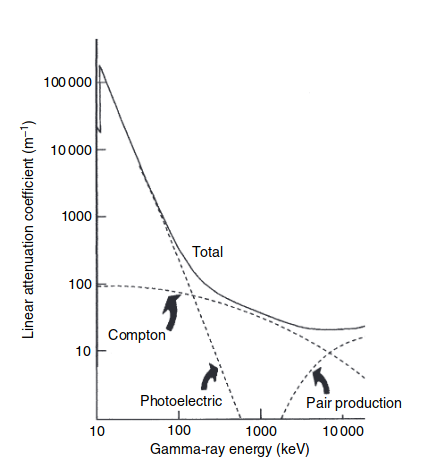
\includegraphics[height=8cm]{Extin.png}
  \caption{Der Extinkionskoeffizient in Abhängigkeit der Energie für verschiedene Prozesse. \cite{Gilmore2}}
  \label{fig:Extin}
\end{figure}

Wie in Abbildung \ref{fig:Extin} zu sehen ist, dominieren bei verschiedenen Energien
unterschiedliche Prozesse. Für geringe Energien dominiert der Photoeffekt, welcher mit
steigender Energie abnimmt, dadurch gewinnt der Comptoneffekt an Bedeutung. Für hohe
Energien dominiert die Paarerzeugung.
Da diese drei Prozesse für die Wechselwirkung von Gammaquanten mit Materie von großer Bedeutung sind
werden sie im Folgenden näher betrachtet.
\cite{Springer3}
\\
\\
\textbf{1. Photoeffekt}\\
Ein Gammaquant wird von einem kernnahen Hüllenelektron (bevorzugt aus der K-Schale) absorbiert,
wodurch das Hüllenelektron ausgelöst wird. Voraussetzung für diesen Effekt ist, dass das Gammaquant
mindestens die Bindungsenergie des Elektrons besitzt, überschüssige Energie wird als kinetische
Energie an das Elektron übertragen.
Das so entstandene "Loch" in der Elektronenhülle wird durch ein energiereicheres Hüllenelektron
gefüllt welches bei dem Übergang aus einer höheren Schale in eine niedrigere Schale
charakteristische Röntgenstrahlung emittiert.
Da sowohl die Röntgenstrahlung als auch das ausgelöste Elektron im Detektor verbleiben und
dort detektiert werden, verbleibt beim Photoeffekt die gesamte Gammaenergie im Detektor, weshalb
der Photopeak besonders wichtig für die Gammaspektroskopie ist.
Der differentielle Wirkungsquerschnitt der Energie lässt sich über die Formel
\begin{equation}
  \frac{d \sigma}{d E} = \bigg(-\frac{64}{7E^{9}}\bigg)^{1/2}\alpha^4 Z^5\sigma_{Th}
  \label{eqn:diffPhoto}
\end{equation}
beschreiben, wobei $\sigma_{Th}$ den Thomson-Wirkungsquerschnitt $\sigma_{Th} = \frac{8}{3}\pi r_{e}^2$
beschreibt mit $r_e$ als klassischen Elektronenradius.
(Thomson-Streuung: Streuung niederenergetischer Photonen an Elektronen) \cite{Springer3}
Der totale Wirkungsquerschnitt für den Photoeffekt ist von der Ordnungszahl des Materials
und der Photonenergie abhängig:
\begin{equation}
  \sigma_{\text{Photo}}\sim Z^5\cdot E_{\gamma}^{-7/2}.
  \label{eqn:WQphoto}
\end{equation}
\cite{Karlsruhe}
\\
\\

\textbf{2. Comptoneffekt}\\
Der Comptoneffekt beschreibt die Streuung von Photonen an äußeren Hüllenelektronen. Da
diese Streuung sehr stark winkelabhängig ist, kann von der gemessenen Elektronenenergie
nicht auf die Energie des Gammaquants geschlossen werden wodurch sich ein kontinuierliches
Spektrum, das Comptonkontinuum bildet. Dieses Spektrum bricht an der Comptonkante ab, hier
beträgt der Streuwinkel 180° und der Energieübertrag $E_{\text{max}}$ ist maximal, trotzdem gibt das
Gammaquant nicht seine gesamte Energie ab
\begin{equation}
  E_{max}=E_{\gamma}\cdot\frac{2\epsilon}{1+2\epsilon}\;\;<E_{\gamma}.
  \label{eqn:kante}
\end{equation}
\cite[Springer3]
Hier ist der Wirkungsquerschnitt über die Klein-Nishina-Formel gegeben, aus dieser ergibt sich der
differentielle Wirkungsquerschnitt:
\begin{equation}
  \frac{d\sigma}{dE}=\frac{3}{8}\sigma_{\text{Th}}\frac{1}{m_0 c^2 e^2}\bigg(2+\bigg(\frac{E}{h\nu-E} \bigg)^2 \bigg[\frac{1}{\epsilon^2}+
  \frac{h\nu-E}{h\nu}-\frac{2}{\epsilon}\bigg(\frac{h\nu-E}{h\nu}\bigg) \bigg]\bigg)
  \label{eqn:diffCompton}
\end{equation}
mit $\epsilon=\sfrac{E_{\gamma}}{m_e c^2}$.
Für den totalen Wirkungsquerschnitt gilt der Zusammenhang
\begin{equation}
  \sigma_{\text{Compton}}\sim \frac{Z}{E_{\gamma}}.
  \label{eqn:WPCompton}
\end{equation}
\\
\\
\textbf{3. Paarerzeugung}\\
Sind die Photonen energiereich genug können Elektron-Positron-Paare erzeugt werden, dafür müssen
die Photonen eine Mindestenergie von $E=2 m_0 c^2$ besitzen, also die doppelte
Ruheenergie des Elektrons.
Das so entstandene Positron annihiliert mit den im Detektor vorhandenen Elektronen und es
entstehen zwei Photonen. Wenn beide Photonen den Detektor verlassen wird dies als double-escape
bezeichnet, verlässt nur eins den Detektor entsteht der single-escape Peak.
Der differentielle Wirkungsquerschnitt für den Prozess der Paarerzeugung ist durch
\begin{equation}
  \frac{d\sigma}{dE}= \frac{28\alpha Z^2 r_{e}^2}{9E_{\gamma}}
  \label{eqn:diffPaar}
\end{equation}
gegeben, während der totale Wirkungsquerschnitt folgende Proportionalität besitzt:
\begin{equation}
  \sigma_{\text{Paar}}\sim Z^2\cdot\ln\Bigg(\frac{2E_{\gamma}}{m_e c^2}\Bigg).
  \label{eqn:WQPaar}
\end{equation}
\\

Eine Übersicht über die möglichen Wechselwirkungen von Gammaquanten mit Materie liefert
Abbildung \ref{fig:Effekt}.
\begin{figure}[H]
  \centering
  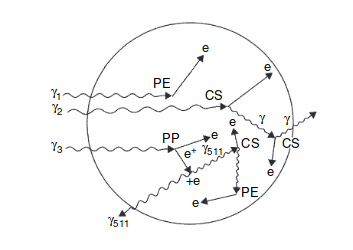
\includegraphics[height=5cm]{Effekte.png}
  \caption{Übersicht der Prozesse im Detektor. \cite{Gilmore2}}
  \label{fig:Effekt}
\end{figure}


\subsection{Grundlagen der Halbleiterinstrumente}
Halbleiter werden zwischen direkten und indirekten Halbleitern unterschieden, dies wird
in Abbildung \ref{fig:Band} dargestellt. Bei direkten Halbleitern
liegt das Maximum des Valenzbands genau unter dem Minimum des Leitungsbandes, somit ist ein direkter Bandübergang möglich.
Bei indirekten Halbleitern liegen Minima und Maxima nicht übereinander, für diesen indirekten Bandübergang ist
ein weiteres Photon nötig.\\

\begin{figure}
  \centering
  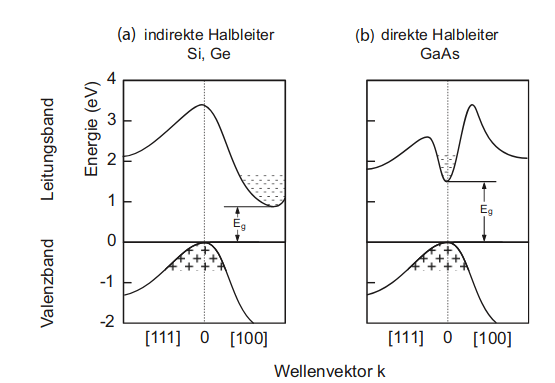
\includegraphics[height=6cm]{Band.png}
  \caption{Bandstruktur für direkte und indirekte Halbleiter.}
  \label{fig:Band}
  \cite{Springer3}
\end{figure}

Außerdem werden die Eigenschaften von Halbleitern durch ihre Dotierung beeinflusst. Germanium besitzt
beispielsweise 4 Valenzelektronen, wird nun ein Material mit fünf Valenzelektronen hinzugegeben bleibt nach
Eingehen der Bindungen ein freies Elektron übrig, somit dominieren die Elektronen als Ladungsträger und es handelt
sich um einen n-dotierten Halbleiter.
Wird stattdessen ein dreiwertiges Element verwendet bleibt ein Loch, somit stehen die Löcher als
positive Ladungsträger zur Verfügung und es handelt sich um einen p-dotierten Halbleiter.\\

\begin{figure}[H]
  \centering
  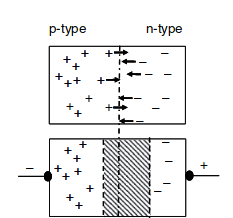
\includegraphics[height=6cm]{pn.png}
  \caption{Bildung einer Verarmungsschicht im pn-Übergang und Verbreiterung dieser durch
  anlegen einer äußeren Spannung.}
  \label{fig:pn}
  \cite{Gilmore2}
\end{figure}

Wie in Abbildung \ref{fig:pn} gezeigt entsteht ein pn-Übergang wenn p- und n-dotierte Halbleiter zusammengebracht werden,
Elektronen und Löcher vernichten sich in einem Teilbereich wodurch eine Verarmungszone entsteht.
Durch anlegen einer äußeren Spannung kann die Größe der Verarmungszone verändert werden. Für die
Verwendung als Detektor ist eine große Verarmungszone gewünscht, da dieser Bereich den
Detektorbereich bildet, also wird die Spannung in Sperrrichtung angelegt.


\subsection{Der Halbleiterdetektor}
Bei dem verwendeten Detektor handelt es sich um einen koaxialen Ge-Detektor wie in Abbildung
\ref{fig:Aufbau} zu sehen ist. Der gesamte Detektor befindet sich unter einer Aluminium
Schutzhaube und ist von außen mit Li-Atomen n-dotiert, wodurch die Oberfläche
gut leitend wird. Im Inneren befindet sich eine Bohrung, diese innere Oberfläche ist
mit Au-Atomen p-dotiert. (Die Dotierung ist hier etwas anders als oben beschrieben, da es sich um
Metall-Halbleiterkontakte handelt.) An diese dotierten Schichten wird die
äußere Spannung angelegt, die n-dotierte Schicht dient als Anschluss für den Pluspol.
Durch die p- und n-dotierten Bereiche bildet sich eine
Verarmungszone im Detektor die den Detektorbereich bildet. Somit müssen die Gammaquanten erst
die Al-Schicht und die Li-Schicht durchdringen um detektiert zu werden, dadurch kommt es zu einer
unteren Nachweisenergie der Gammaenergie, diese liegt bei 40 bis 50\;keV.
Dieser Gesamte Aufbau, wie in Abbildung \ref{fig:Aufbau} gezeigt befindet sich in einem
Bleigehäuse welches von innen mit Kupferplatten ausgelegt ist. Das Bleigehäuse dient zur Abschiermung
äußerer Strahlung, während die Kupferplatten die aus dem Blei austretende Strahlung
abhalten sollen.

\begin{figure}
  \centering
  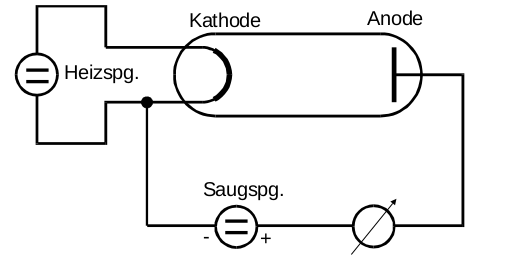
\includegraphics[height=7cm]{Aufbau.png}
  \caption{Schematischer Aufbau des Ge-Detektors. \cite{skript}}
  \label{fig:Aufbau}
\end{figure}

Dringt ein Gammaquant in die Verarmungszone ein wechselwirkt es mit der Materie und kann
z.B. ein Elektron auslösen welches mit anderen Elektronen stößt und ein Elektronen-Loch-Paar erzeugt.
Durch die angelegte Spannung wird das Paar räumlich getrennt wodurch eine Rekombination verhindert wird,
der dadurch entstehende Ladungsimpuls
wird verstärkt und bildet das Detektorsignal. Dieses ist proportional zu der einfallenden Photonenergie, da mit
einer höheren Energie auch mehr Elektronen-Loch-Paare erzeugt werden können.
Dringt das Gammaquant außerhalb der Verarmungszone in den Detektor ein rekombinieren die
Elektronen-Loch-Paare sofort, somit kann kein Signal gemessen werden.\\
Um Störsignale zu minimieren wird der Detektor mit Stickstoff auf 77\;K gekühlt, denn durch die
hohe externe Spannung kommt es zu thermischen Effekten wodurch sich noch Ladungsträger in der Verarmungszone
befinden und das Signal stören können.
\\
\\
\textbf{Eigenschaften eines Halbleiterdetektors}\\
Eine charakteristische Größe des Detektors ist das Auflösungsvermögen, dieses wird durch die
Halbwertsbreite $\Delta E_{1/2}$ der Impulshöhenverteilung beschrieben. Energien mit den Mittelwerten
$E_1$ und $E_2$ können noch voneinander unterschieden werden, wenn der Energieunterschied mindestens
$\Delta E_{1/2}$ beträgt.

Die Vollenergienachweiswahrscheinlichkeit eines Detektors gibt die Nachweiswahrscheinlichkeit eines Detektors
in Abhängigkeit der Energie an. Um sie zu bestimmen wird aus der aktuellen Aktivität der Probe der
theoretische Linieninhalt bestimmt, der Quotient aus gemessenem Linieninhalt und theoretischem
Linieninhalt gibt die Nachweiswahrscheinlichkeit des Detektors an.

\subsection{Das Spektrum eines monochromatischen Gammastrahlers}
Das Spektrum eines monochromatischen Gammastrahlers zeigt mehrere Besonderheiten auf, wie in Abbildung \ref{fig:Spektrum} zu
sehen. Wesentliche Bestandteile sind das Comptonkontinuum mit der Comptonkante, der Rückstreupeak
und der Photopeak. Der Photopeak entsteht dadurch, dass die Gammaquanten ihre gesamte Energie im Detektor deponieren
und wird daher auch Vollenergiepeak genannt. Er entsteht wenn die Gammaquanten im Detektor durch
Comptonstreuung genügend Energie verlieren bis der Photoeffekt eintreten kann und die restliche Energie
an den Detektor abgegeben wird. Auf diese Weise deponieren die Gammaquanten ihre gesamte Energie im
Detektor, so dass das Maximum des Photopeaks die Energie der Gammastrahlung angibt.\\
Das Comptonkontinuum entsteht durch Comptonstreuung der Gammaquanten, erfolgt die Streuung im
180° Winkel wobei der Energieübertrag maximal ist entsteht die Comptonkante. Da durch mehrfache
Comptonstreuung ein größerer Energieübertrag möglich ist als duch eine einmalige Streuung im 180° Winkel ist die
Componkante ausgeschmiert.\\
Da die Strahlung der Probe keine Vorzugsrichtung hat, wechselwirken einige Gammaquanten auch mit der
Abschirmung des Detektors und verlieren so Energie, werden sie dann so zurückgestreut, dass sie den
Detektor erreichen bilden sie den Rückstreupeak, dieser liegt bei
\begin{equation}
  E_{\text{Rück}}=E_{\gamma}\frac{1}{1+2\epsilon}
  \label{eqn:Rückstreu}
\end{equation}
Zwei weitere mögliche Peaks sind double- und single-escape Peak. Fällt ein Gammaquant in den Detektor und wechselwirkt über
Paarerzeugung entsteht ein Elektron und ein Positron, das Positron annihiliert mit den Elektronen der umgebenden Materie wobei
zwei Photonen erzeugt werden. Verlässt eins dieser Photonen den Detektor komm es zu single-escape Peak, verlassen beide
Photonen den Detektor entsteht der double-escape Peak.
\cite{Gilmore2}


\begin{figure}
  \centering
  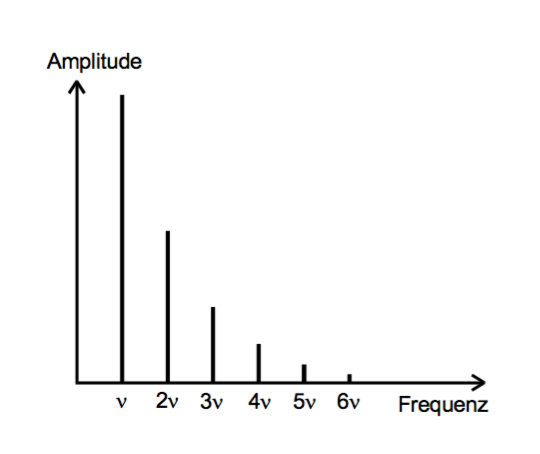
\includegraphics[height=7cm]{Spektrum.png}
  \caption{Gammaspektrum von $\ce{^{28}Al}$. Die Componkante ist hier nicht eingezeichnet, sie ist der Peak zwischen single escape und Photopeak,
  das Comptonkontinuum verläuft von der y-Achse bis zur Comptonkante.}\cite{Gilmore2}
  \label{fig:Spektrum}
\end{figure}

\section{Durchführung}
\label{sec:Durchführung}
Zunächst wird eine kalibrierte $\ce{^{152}Eu}$-Probe vermessen die später zur Energiekalibration
genutzt wird. Die Probe wird in die Probenhalterung des Detektors eingespannt, um für alle
Proben den gleichen Abstand zum Detektor zu garantieren wird ein Messingstab als Abstandshalter
verwendet, dieser wird vor der Messung natürlich wieder entfernt.
Auf dem Computer wird nun die Messung gestartet, die Messzeit beträgt ca. 3600\;s $\sim$ eine Stunde.\\
Für $\ce{^{137}Cs}$ und und eine weitere Probe (entweder $\ce{^{125}Sb}$ oder $\ce{^{133}Ba}$ )
wird äquivalent vorgegangen. Zuletzt wird eine unbekannte Probe vermessen, da diese eine andere
Form besitzt und nicht in den Probenhalter passt wird sie vor der Aluminiumschutzhaube des Detektors
platziert.

\section{Auswertung}
\label{sec:Auswertung}

\subsection{Energiekalibration und Bestimmung der Vollenergienachweiswahrscheinlichkeit}
Zur Kalibration wird ein $\ce{^{152}Eu}$-Strahler verwendet, dessen Aktivität am 01.10.2000
%\begin{align*}
%  \SI{4130(60)}{\becquerel}
%\end{align*}
$\SI{4130(60)}{\becquerel} $ betrug. \\
Nach dem Gesetz des radioaktiven Zerfalls berechnet sich die Aktivität am Messtag (08.04.2019) durch

\begin{equation}
  \symup{A} (t) = \symup{A}(0)\cdot \symup{e}^{-\lambda t} \: ,
\end{equation}

wobei $\lambda=\SI{1.6244(19)e-9}{\per\second}$ \cite{lara} die Zerfallskonstante
von $\ce{^{152}Eu}$ bezeichnet.

Der Fehler ergibt sich hierbei nach der Gauß´schen Fehlerfortpflanzung
\begin{equation}
  \increment f = \sqrt{ \sum_{i=1}^N \left( \frac{\partial f}{\partial x_i}\right)^2
  \cdot (\increment x_i)^2  } \: ,
  \label{eqn:gaus}
\end{equation}
also gemäß
\begin{equation}
  \increment \symup{A} (t) = \sqrt{ (\symup{e}^{-\lambda t})^{2}\cdot (\increment \symup{A}(0))^2
   + (-t\cdot\symup{A}(0)\cdot \symup{e}^{-\lambda t})^2\cdot(\increment \lambda)^2}
\end{equation}
Die Anzahl der Tage vom 01.10.2000 bis zum 08.04.2019 beträgt 6763 Tage, was
584323200 Sekunden entspricht, sodass sich insgesamt der Wert $\SI{1599(29)}{\becquerel} $
für die Aktivität der Probe am Messtag ergibt. \\
Der abgedeckte Raumwinkel lässt sich aus dem gemessenen Abstand a der Probe
zum Detektor, wobei auch der Abstand von $\SI{1.5}{\centi\meter}$ zwischen Al-Haube und Detektor
berücksichtigt wird,
und dem angegebenen Radius r des Detektorvolumens bestimmen. Die entsprechenden Werte
betragen
\begin{align*}
  a &= \SI{8.8}{\centi\meter} \\
  r &= \SI{2.25}{\centi\meter} \: .
\end{align*}

Die Formel zur Berechnung des abgedeckten Raumwinkelanteils ergibt sich dabei
über geometrische Überlegungen zu
\begin{equation}
  \frac{\Omega}{4\pi}= \frac{1}{2}(1-\frac{a}{\sqrt{a^2+r^2}})   \: ,
\end{equation}
in diesem Fall also $\frac{\Omega}{4\pi}= 0.01558$.
Diese somit errechneten Werte sind später wichtig zur Bestimmung der Vollenergienachweiswahrscheinlichkeit. \\
Das gemessene Spektrum des kalibrierten $\ce{^{152}Eu}$-Strahlers ist in Abbildung
\ref{fig:plot1} dargestellt. Es sind jedoch nur die ersten 4000 Kanäle dargestellt,
da bei höheren Kanälen keine signifikanten Messwerte mehr zu sehen sind. Die Messwerte
reichen bis Kanalnummer 8191 und die Messzeit beträgt $\SI{3598}{\second}$.
\begin{figure}
  \centering
  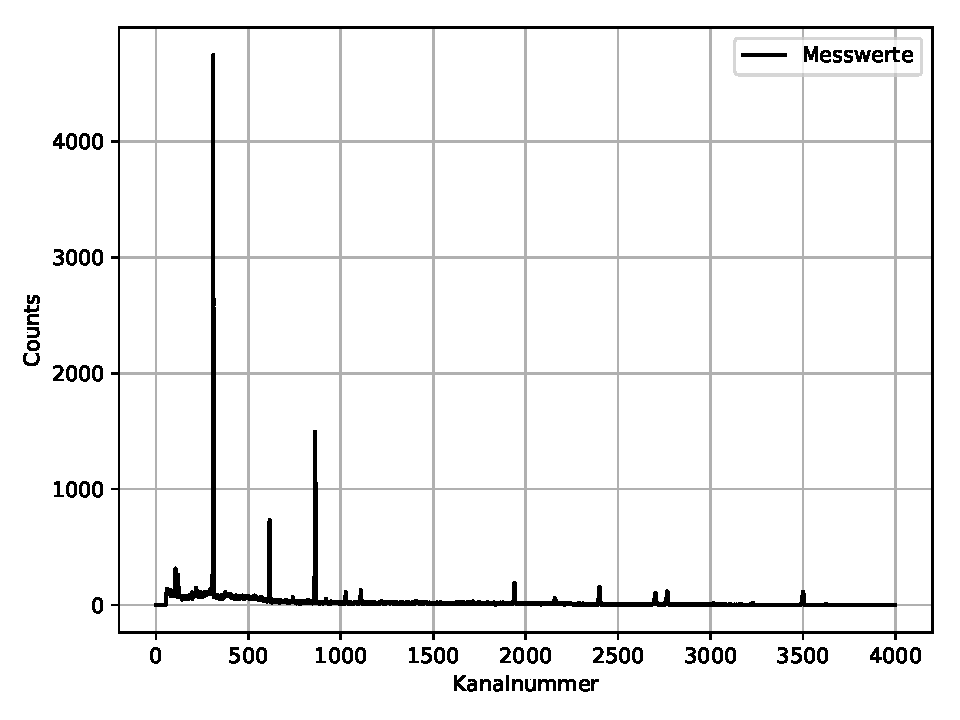
\includegraphics[height=9cm]{Eu.pdf}
  \caption{Spektrum des $\ce{^{152}Eu}$-Strahlers}
  \label{fig:plot1}
\end{figure}

Um mit diesem die Energiekalibration durchzuführen, werden die Peaks des Spektrums
jeweils mit einer Gaußverteilung der Form
\begin{equation}
  \symup{g} (x) = a + b \cdot \symup{e}^{(\frac{x-z}{c})^2}
  \label{eqn:gausk}
\end{equation}
gefittet.

Die sich daraus ergebenen Parameter sind in Tabelle \ref{tab:tabe1} angegebenen.
\begin{table}[H]
  \centering
  \caption{Messwerte der Wärmepumpe}
  \label{tab:tabe1}
    \begin{tabular}{S S S S S S}
    \toprule
    $ t  \: / \si{\second} $ & $ p_a \: / \si{\bar} $ & $ p_b \: / \si{\bar} $ &
    $ T_1 \: / \si{\kelvin} $ & $ T_2 \: / \si{\kelvin} $ & $ P \: / \: \si{\watt} $\\
    \midrule
    0 & 5.0 & 5.0 & 293.65 & 293.65 & 0 \\
    60 & 4.7 & 6.0 & 294.15 & 293.55 & 115 \\
    120 & 4.4 & 6.4 & 295.15 & 293.15 & 118 \\
    180 & 4.5 & 6.9 & 296.35 & 291.95 & 122 \\
    240 & 4.6 & 7.0 & 297.55 & 290.95 & 125 \\
    300 & 4.6 & 7.0 & 298.85 & 289.95 & 125 \\
    360 & 4.5 & 7.2 & 300.05 & 289.15 & 123 \\
    420 & 4.4 & 7.4 & 301.15 & 288.45 & 123 \\
    480 & 4.3 & 7.8 & 302.35 & 287.65 & 122 \\
    540 & 4.2 & 8.0 & 303.55 & 286.95 & 122 \\
    600 & 4.2 & 8.1 & 304.65 & 286.25 & 121 \\
    660 & 4.1 & 8.3 & 305.75 & 285.55 & 121 \\
    720 & 4.0 & 8.5 & 306.75 & 284.95 & 121 \\
    780 & 4.0 & 8.8 & 307.75 & 284.35 & 121 \\
    840 & 3.9 & 9.0 & 308.75 & 283.75 & 121 \\
    900 & 3.8 & 9.1 & 309.65 & 283.15 & 121 \\
    960 & 3.8 & 9.2 & 310.55 & 282.55 & 122 \\
    1020 & 3.8 & 9.5 & 311.45 & 282.05 & 122 \\
    1080 & 3.7 & 9.8 & 312.25 & 281.55 & 122 \\
    1140 & 3.7 & 10.0 & 313.05 & 281.15 & 122 \\
    1200 & 3.7 & 10.0 & 313.9 & 280.65 & 122 \\
    1260 & 3.6 & 10.2 & 314.65 & 280.25 & 123 \\
    1320 & 3.6 & 10.3 & 315.35 & 279.85 & 123 \\
    1380 & 3.6 & 10.6 & 316.15 & 279.45 & 124 \\
    1440 & 3.6 & 10.8 & 316.85 & 279.15 & 124 \\
    1500 & 3.6 & 11.0 & 317.55 & 278.75 & 124 \\
    1560 & 3.6 & 11.1 & 318.25 & 278.55 & 124 \\
    1620 & 3.6 & 11.2 & 318.95 & 278.25 & 125 \\
    1680 & 3.5 & 11.4 & 319.55 & 277.95 & 125 \\
    1740 & 3.5 & 11.5 & 320.15 & 277.65 & 125 \\
    1800 & 3.5 & 11.7 & 320.75 & 277.45 & 125 \\
    1860 & 3.5 & 11.9 & 321.35 & 277.25 & 125 \\
    1920 & 3.5 & 12.0 & 321.95 & 277.05 & 125 \\
    1980 & 3.5 & 12.1 & 322.45 & 276.95 & 125 \\








      \bottomrule
    \end{tabular}
\end{table}


Die zentrale Lage der Peaks im Hinblick auf die Kanalnummer ist durch den Parameter
z gegeben. Diese Werte werden zusammen mit der jeweiligen relativen Höhe mit den theoretischen
Emissionslinien der Datenbank \cite{lara} verglichen und es wird jedem Peak eine Linie
zugeordent. Diese Zuordnung ist zusammen mit der jeweiligen relativen Emissionswahrscheinlichkeit P
in Tabelle \ref{tab:tabe2} dargestellt.
\begin{table}[H]
  \centering
  \caption{Wertetabelle für $\alpha$ und $C_V$.}
  \label{tab:tab2}
    \begin{tabular}{S S S S S}
    \toprule
    $ T\: \text{in}\: \si{\K} $ & $ {\alpha \cdot 10^{-6} \: \text{in}\: \si {\per\K}} $ &
    $ C_V \: \text{in}\: \si{\J\per\K\mol} $\\
    \midrule %Cv, a *10-6, Cv
    %0 & 1 & 1\\
    88.60\pm0.24 & 9.56\pm0.06 & 14.17\pm8.13  \\ %&3.6 & 318.97\pm0.85\\
    93.81\pm0.24 & 10.10\pm0.06 & 17.58\pm10.03 \\ %& 4.7 & 440.90\pm1.11\\
    99.74\pm0.24 & 10.66\pm0.05 & 15.52\pm8.84 \\ %& 5.1 & 508.68\pm1.21\\
    104.74\pm0.24 & 11.07\pm0.05 & 18.44\pm10.52 \\ %& 4.6 & 481.79\pm1.09\\
    110.94\pm0.24 &  11.54\pm0.05 & 14.86\pm8.45 \\ %& 5.3 & 587.97\pm1.27\\
    115.96\pm0.24 & 11.89\pm0.05 & 18.49\pm10.52 \\ %& 4.6 & 533.41\pm1.10\\
    121.47\pm0.24 &  12.22\pm0.05 & 16.83\pm9.57 \\ %& 4.9 & 595.21\pm1.17\\
    126.99\pm0.24 & 12.53\pm0.04 & 16.79\pm9.54 \\ %& 4.9 & 622.29\pm1.18\\
    131.58\pm0.24 & 12.77\pm0.04 & 20.42\pm11.62 \\ %& 4.2 & 552.62\pm1.01\\
    136.65\pm0.24 & 13.02\pm0.04 & 18.40\pm10.47 \\ %& 4.6 & 628.57\pm1.11\\
    141.49\pm0.24 & 13.24\pm0.04 & 19.28\pm10.97 \\ %& 4.4 & 622.54\pm1.07\\
    146.34\pm0.24 & 13.44\pm0.04 & 19.24\pm10.95 \\ %& 4.4 & 643.88\pm1.07\\
    150.95\pm0.24 & 13.62\pm0.04 & 20.22\pm11.52 \\ %& 4.3 & 649.11\pm1.05\\
    155.34\pm0.24 & 13.79\pm0.04 & 21.31\pm12.14 \\ %& 4.1 & 636.88\pm0.98\\
    159.97\pm0.24 & 13.95\pm0.04 & 20.12\pm11.47 \\ %& 4.3 & 687.89\pm1.05\\
    164.62\pm0.24 & 14.10\pm0.04 & 20.18\pm11.51 \\ %& 4.3 & 707.87\pm1.06\\
    168.79\pm0.25 & 14.23\pm0.04 & 22.54\pm12.86 \\ %& 3.9 & 658.27\pm0.95\\
    173.45\pm0.25 &  14.37\pm0.04 & 20.08\pm11.46 \\ %& 4.3 & 745.84\pm1.06\\
    178.13\pm0.25 &  14.50\pm0.04 & 20.04\pm11.44 \\ %& 4.3 & 765.94\pm1.06\\
    182.56\pm0.25 &  14.62\pm0.04 & 21.11\pm12.06\\
    192.70\pm0.25 &  14.87\pm0.04 & 18.41\pm10.47\\
    200.15\pm0.25 &  15.04\pm0.04 & 25.19\pm14.28\\
    208.87\pm0.25 &  15.23\pm0.04 & 21.43\pm12.18\\
    217.12\pm0.25 &  15.38\pm0.04 & 22.65\pm12.88\\
    225.15\pm0.25 &  15.53\pm0.03 & 23.27\pm13.24\\
    232.70\pm0.25 &  15.70\pm0.03 & 24.75\pm14.08\\
    240.53\pm0.25 &  15.74\pm0.03 & 23.84\pm13.58\\
    248.39\pm0.25 &  15.89\pm0.03 & 23.74\pm13.53& \\
    256.01\pm0.25 &  15.97\pm0.03 & 24.46\pm13.94 \\
    263.41\pm0.26 &  16.01\pm0.03 & 25.22\pm14.38 \\
    271.08\pm0.26 &  16.18\pm0.03 & 24.26\pm13.86 \\
    278.52\pm0.26 &  16.27\pm0.03 & 25.03\pm14.29&\\
    285.98\pm0.26 &  16.35\pm0.03 & 24.92\pm14.25 \\
    293.21\pm0.26 &  16.42\pm0.03 & 25.74\pm14.72 \\
    300.98\pm0.26 &  16.50\pm0.03 & 23.87\pm13.68 \\
    308.51\pm0.26 &  16.57\pm0.03 & 24.63\pm14.12\\



      \bottomrule
    \end{tabular}
\end{table}

Mit den Wertepaaren aus Kanalnummer und Linienenergie wird nun eine lineare Ausgleichsrechnung der
Form
\begin{equation}
  f(x) = a\cdot x +b
  \label{eqn:li}
\end{equation}
durchgeführt, woraus sich die Parameter
\begin{align}
  a &= \SI{0.403169(29)}{\kilo\electronvolt} \\
  b &= \SI{-3.034(60)}{\kilo\electronvolt}
\end{align}
ergeben. Die Wertepaare sind zusammen mit der resultierenden Gerade in Abbildung \ref{fig:plot3}
dargestellt. Die Fehler der Messwerte sind aufgrund ihrer sehr geringen relativen Größe dabei zu vernachlässigen.
\begin{figure}
  \centering
  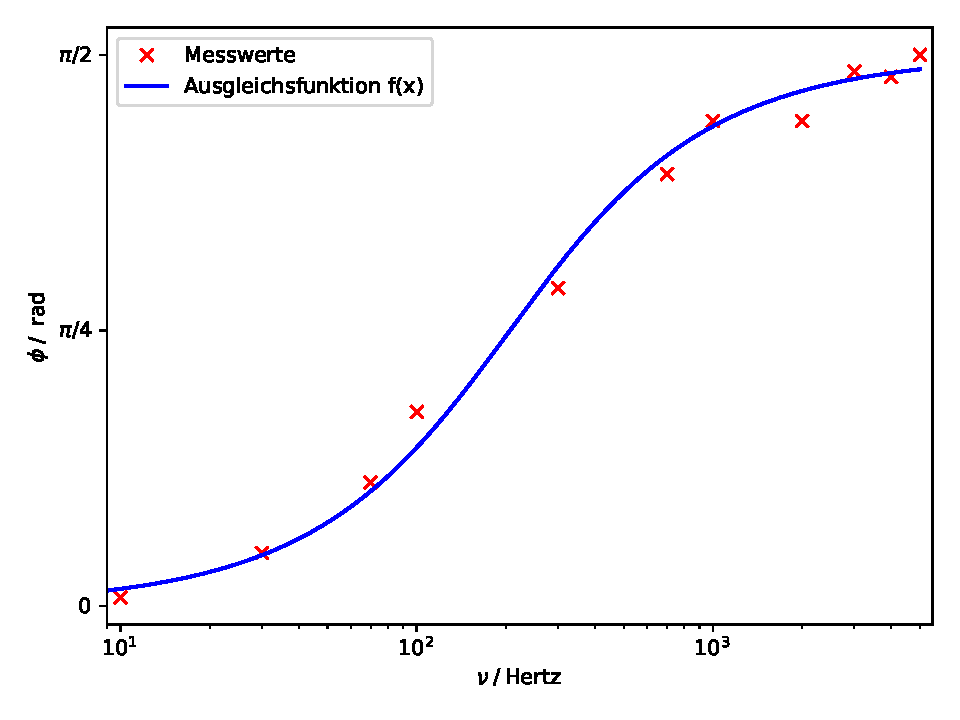
\includegraphics[height=9cm]{plot3.pdf}
  \caption{Lineare Ausgleichsrechnung zur Energiekalibration}
  \label{fig:plot3}
\end{figure}
Die Energiekalibration erfolgt somit gemäß
\begin{equation}
  \symup{E}_{\gamma} (x) = \SI{0.403169}{\kilo\electronvolt}\cdot x - \SI{3.034}{\kilo\electronvolt}
  \label{eqn:gerade}
\end{equation}
wobei x die Kanalnummer bezeichnet.
Der dazugehörige Fehler ergibt mittels Gleichung \ref{eqn:gaus} durch
\begin{equation}
   \increment \symup{E}_{\gamma} (x) =\sqrt{ (\SI{0.000029}{\kilo\electronvolt}\cdot x)^2 +
   (\SI{0.060}{\kilo\electronvolt})^2}
   \label{eqn:fgerade}
\end{equation}
\\
Zur Bestimmung der Vollenergienachweiswahrscheinlichkeit wird zunächst die Gleichung \ref{eqn:gausk}
integriert, um den Inhalt der Peaks zu bestimmen, wobei der Untegrund $a$ vorher abgezogen wird.
Es ergibt sich somit ein Linieninhalt von
\begin{equation}
  \symup{I} =\int_{-\infty}^{\infty} c \cdot \symup{e}^{(\frac{x-z}{b})^2} \symup{d}x
  = c \cdot b \cdot \sqrt{\pi}
  \label{eqn:inh}
\end{equation}
in Abhängigkeit der Parameter b und c.
Der Fehler ergibt sich durch Gleichung \ref{eqn:gaus} über die Gleichung
\begin{equation}
  \increment \symup{I} = \sqrt{ (\increment c \cdot b \cdot \sqrt{\pi})^{2}
   + (c \cdot \increment b \cdot \sqrt{\pi}})^{2} \: .
     \label{eqn:inhf}
\end{equation}
Mit den Werten aus Tabelle \ref{tab:tabe1} lassen sich somit die einzelnen Linieninhalte berrechen,
welche in Tabelle \ref{tab:tabe3} angegeben sind.
\begin{table}
  \centering
  \caption{Messwerte für den ersten Doppelspalt.}
   \begin{tabular}{S S| S S | S S}
    \toprule
    $x/\; \si{\mm}$& $A/\;\si{\nA}$ &
    $x/\; \si{\mm}$& $A/\;\si{\nA}$ &
    $x/\; \si{\mm}$& $A/\;\si{\nA}$ \\
    \midrule

    15.0& 4.6& 23.0& 25.0& 29.5& 6.0\\
    15.5& 4.2& 23.5& 30.0& 30.0& 5.3\\
    16.0& 4.0& 24.0& 35.0& 30.5& 4.9\\
    16.5& 4.0& 24.25& 36.0& 31.0& 4.7\\
    17.0& 4.4& 24.5& 37.0& 31.5& 4.4\\
    17.5& 5.5& 24.75& 38.0& 32.0& 4.2\\
    18.0& 6.6& 25.00& 37.0& 32.5& 3.8\\
    18.5& 7.7& 25.25& 36.0& 33.0& 3.6\\
    19.0& 8.2& 25.5& 36.0& 33.5& 3.2\\
    19.5& 8.4& 26.0& 33.0& 34.0& 3.2\\
    20.0& 8.4& 26.5& 28.5& 34.5& 3.2\\
    20.25& 8.4& 27.0& 23.0& 35.0& 3.3\\
    20.5& 8,7& 27.5& 18.0& 35.5& 3.4\\
    21.0& 9.8& 28.0& 13.5& 36.0& 3.5\\
    21.5& 12.0& 28.5& 10.0\\
    22.0& 15.0& 29.0& 7.8\\
    22.5& 20.0& 29.25& 6.7\\


   \bottomrule
  \end{tabular}
  \label{tab:tabelle3}
\end{table}

Zum Vergleich werden nun die Theoriewerte berrechnet, als Produkt
der Emissionswahrscheinlichkeiten P aus Tabelle \ref{tab:tabe2},
dem abgedeckten Raumwinkelanteil $\frac{\Omega}{4\pi}= 0.01558$, der errechneten Aktivität
$A =\SI{1599(29)}{\becquerel} $
und der Messzeit von $t = \SI{3598}{\second}$
\begin{equation}
  \symup{I}_{\text{theo}} = P\cdot \frac{\Omega}{4\pi} \cdot A \cdot t
  \label{eqn:itheo}
\end{equation}
mit dem Fehler über Gleichung \ref{eqn:gaus} von
\begin{equation}
  \increment \symup{I}_{\text{theo}} = \sqrt{ (\increment P\cdot \frac{\Omega}{4\pi} \cdot A \cdot t)^{2}
   + (P\cdot \frac{\Omega}{4\pi} \cdot \increment A \cdot t)^{2}} \: .
\end{equation}
Aus dem jeweiligen Quotienten
\begin{equation}
  \symup{Q} = \frac{\symup{I}}{\symup{I}_{\text{theo}}}
  \label{eqn:ven1}
\end{equation}
mit dem dazugehörigen Fehler
\begin{equation}
  \increment \symup{Q} = \sqrt{ (\frac{1}{\symup{I}_{\text{theo}} \cdot \increment \symup{I})^{2}
   + (\frac{\symup{I}}{\symup{I}_{\text{theo}}})^{2}}\cdot \increment \symup{I}_{\text{theo}})^{2}}
\end{equation}
ergibt sich somit jeweils die Nachweiswahrscheinlichkeit des Peaks, wie in Tabelle
\ref{tab:tabe4} dargestellt ist.
\begin{table}[H]
  \centering
   \begin{tabular}{c c c c}
    \toprule
    Nummer der Oberwelle & $ U_{\text Theorie,Rechteck}\: / \si{\volt} $ &
    $ U_{\text Theorie,Dreick}\: / \si{\volt} $ & $ U_{\text Theorie,Sägezahn}\: / \si{\volt} $ \\
    \midrule
    1 & 1145 & 182 & 573 \\
    2 & 0 & 0 & 286 \\
    3 & 573 & 20 & 191 \\
    4 & 0 & 0 & 143 \\
    5 & 229 & 7 & 115 \\
    6 & 0 & 0 & 96 \\
    7 & 164 & 4 & 82 \\
    8 & 0 & 0 & 72 \\
    9 & 127 & 2 & 64 \\
    10 & 0 & 0 & 57 \\
    \bottomrule
  \end{tabular}
  \caption{Eingestellte Schwingungsamplituden.}
  \label{tab:tabe4}
\end{table}

Da die Nachweiswahrscheinlichkeit im Allgemeinen energieabhängig ist, wird Q in
Abhängigkeit von $ \text{E}_{\gamma} $ dargestellt und mit einer Potenzfunktion der Form
\begin{equation}
  \symup{Q}(\text{E}_{\gamma}) = c\cdot (\text{E}_{\gamma}-a)^{d}
  \label{eqn:ven2}
\end{equation}
gefittet, wie in Abbildung \ref{fig:plot4} dargestellt ist.
Es ergeben sich hierbei die Parameter
\begin{align*}
  a &= -191 \pm 64 \\
  c &= 2474 \pm 3467 \\
  d &= -1.47 \pm 0.19 \: .
\end{align*}
 %Die Formel für die eigentliche Höhe eines
%gemessenen Peaks ergibt sich aus Gleichungen \ref{eqn:ven1} und \ref{eqn:ven2} durch Umstellen zu
%\begin{equation}
%  \symup{I}_{\text{theo}} = \frac{\symup{I}}{\symup{Q}}=\frac{\symup{I}}{c\cdot (\text{E}_{\gamma}-a)^{d}}
%  \label{eqn:ven}
%\end{equation}
%mit dem dazugehörigen Fehler
%\begin{equation}
%  \symup{I}_{\text{theo}} = \frac{\symup{I}}{\symup{Q}}=\frac{\symup{I}}{c\cdot (\text{E}_{\gamma}-a)^{d}}
%  NAMNAM
%  \label{eqn:ven}
%\end{equation}
\begin{figure}
  \centering
  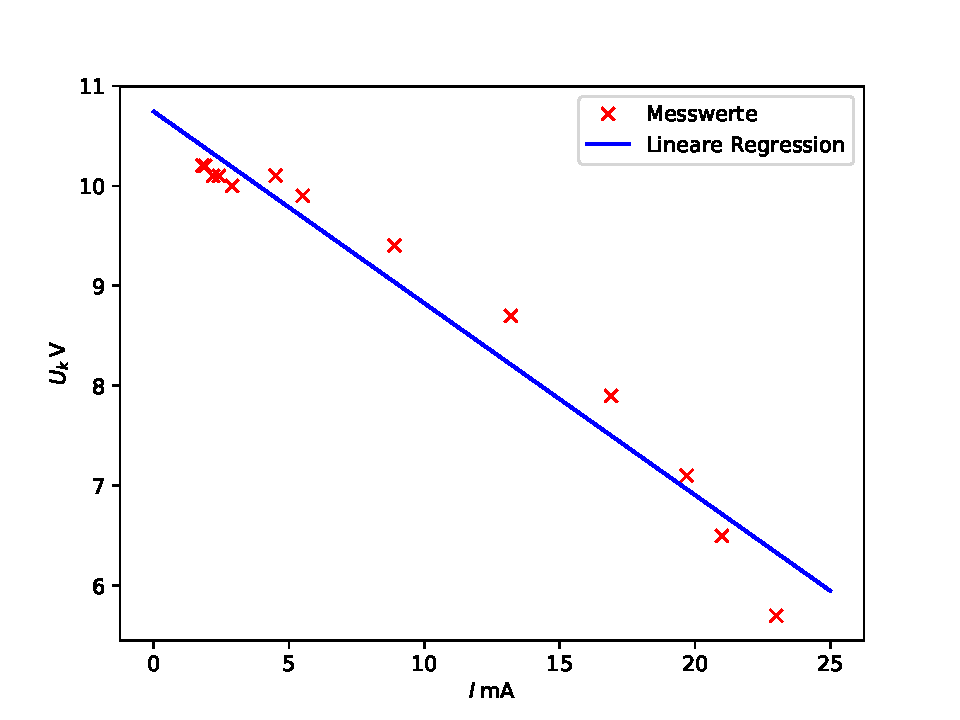
\includegraphics[height=9cm]{plot4.pdf}
  \caption{Werte zur Bestimmung der Vollenergienachweiswahrscheinlichkeit sowie gefittete Potenzfunktion}
  \label{fig:plot4}
\end{figure}

\subsection{Untersuchung eines monochromatischen Gamma-Spektrums}
Zur Untersuchung des monochromatischen Gamma-Spektrums wird das aufgenommene Spektrum
zunächst durch die Gleichung \ref{eqn:gerade} kalibriert, wobei sich der Fehler über
\ref{eqn:fgerade} ergibt. Die so erhaltenen Werte sind in Abbildung \ref{fig:plot5}
dargestellt, wobei auf Fehlerbalken aufgrund der geringen Fehler verzichtet wird. Die
Messzeit beträgt $\SI{2593}{\second}$ und es wurden 8191 Kanäle gemessen, wobei nur die
ersten 2000 dargestellt sind, da bei höheren Kanalnummern keine signifikanten Messwerte
mehr zu erkennen sind.
\begin{figure}
  \centering
  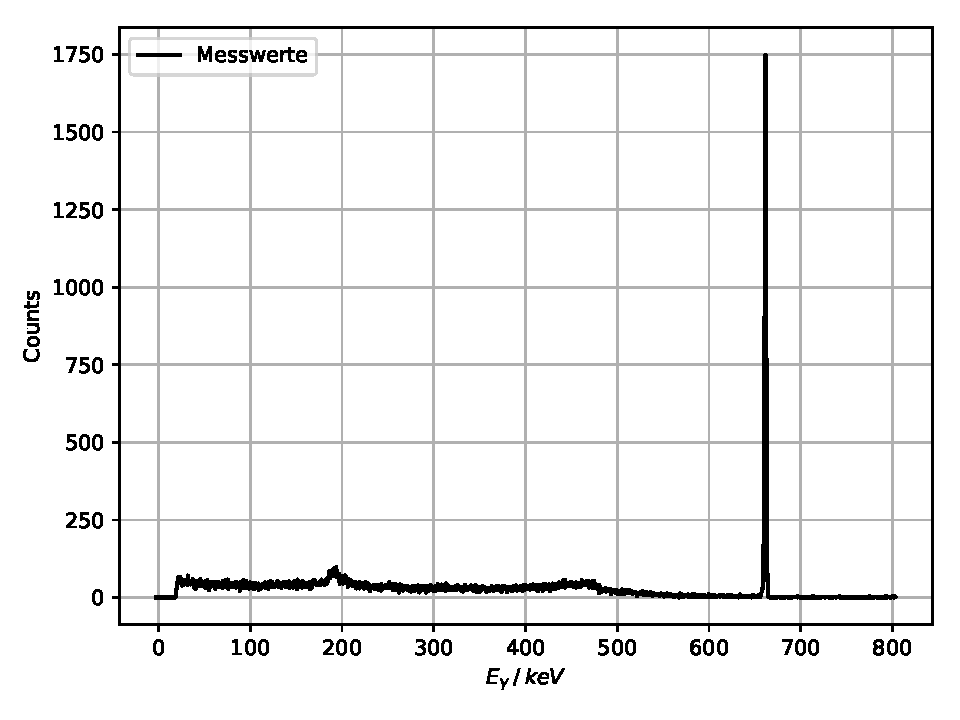
\includegraphics[height=9cm]{Cs.pdf}
  \caption{Kalibriertes Spektrum des $\ce{^{137}Cs}$-Strahlers }
  \label{fig:plot5}
\end{figure}
Zur Bestimmung der Energie wird die Vollenergielinie mit der Gaußverteilung aus Gleichung
\ref{eqn:gausk} gefittet, wobei sich die Parameter
\begin{align*}
  a &= 5.7 \pm 4.2 \\
  b &= 1674 \pm 17 \\
  c &= \SI{1.227(15)}{\kilo\electronvolt}\\
  z &= \SI{661.5985(98)}{\kilo\electronvolt} \:
\end{align*}
ergeben.
Die Energie des Strahlers ist dabei durch den Parameter $z$ gegeben, also
\begin{align*}
  \symup{E}_{Cs} = \SI{661.5985(98)}{\kilo\electronvolt} \: .
\end{align*}
Der Theoriewert von $\ce{^{137}Cs}$ beträgt $\SI{661.657(3)}{\kilo\electronvolt}$ \cite{lara}. \\
Der Bereich um die Vollenergielinie ist in
Abbildung \ref{fig:plot6} dargestellt, woraus sich die Halbwertsbreite und die
Zehntelwertsbreite ablesen lässt, wobei eine Ungenauigkeit durch
Ablesefehler von etwa $\SI{0.2}{\kilo\electronvolt}$ angenommen wird.
Es ergibt sich hierdurch
\begin{align*}
  \symup{E}_{1/2} = \SI{662.6(2)}{\kilo\electronvolt} -\SI{660.6(2)}{\kilo\electronvolt}
  =\SI{2.0(3)}{\kilo\electronvolt}\\
  \symup{E}_{1/10} = \SI{663.3(2)}{\kilo\electronvolt} -\SI{659.6(2)}{\kilo\electronvolt}
  =\SI{3.7(3)}{\kilo\electronvolt} \:
\end{align*}
woraus sich ein Verhältniss von
\begin{equation}
  \frac{\symup{E}_{1/2}}{\symup{E}_{1/10}} =  0.54 \pm 0.09 \:
\end{equation}
ergibt.
\begin{figure}
  \centering
  \includegraphics[height=9cm]{Plot6.pdf}
  \caption{Vollenergielinie}
  \label{fig:plot6}
\end{figure}
Die Halbwertsbreite einer Gaußkurve gemäß Gleichung \ref{eqn:gausk} ist durch die
Formel
\begin{equation}
  \symup{E}_{1/2} = 2c\cdot\sqrt{ln2}
\end{equation}
mit dem Fehler
\begin{equation}
  \increment \symup{E}_{1/2} = 2\increment b\cdot\sqrt{ln2} \: ,
\end{equation}
gegeben und beträgt somit
\begin{align*}
  \symup{E}_{1/2,theo} = \SI{1.701(21)}{\kilo\electronvolt} \: .
\end{align*}
Die Zehntelwertsbreite ergibt sich analog über die Gleichung
\begin{equation}
  \symup{E}_{1/10} = 2c\cdot\sqrt{ln10}
\end{equation}
mit dem Fehler
\begin{equation}
  \increment \symup{E}_{1/10} = 2\increment b\cdot\sqrt{ln10} \: ,
\end{equation}
zu
\begin{align*}
  \symup{E}_{1/10, theo} = \SI{5.651(69)}{\kilo\electronvolt} \: .
\end{align*}
Das Verhältniss dieser beiden Größen ist unabhängig von den jeweiligen Parametern der
Kurve stets
\begin{equation}
  \frac{\symup{E}_{1/2}}{\symup{E}_{1/10}} = \sqrt{\frac{ln2}{ln10}}
  \approx 0.549 \: ,
\end{equation}
Diese theoretisch erhaltenen Werte werden mit den abglesenen verglichen, wobei sich
die Abweichung über die Formel
\begin{equation}
  \frac{\lvert \text{Wert}_{\text{Theorie}}-\text{Wert}_{\text{Messung}}\rvert}{\text{Wert}_{\text{Theorie}}}
  \label{eqn:abw}
\end{equation}
berechnen lässt zu 1.64 \%. Diese Abweichung ist offensichtlich sehr gering und liegt innerhalb der
Ableseunsicherheit, was auf eine gute Beschreibung der Vollenergielinie
durch eine Gaußkurve schließen lässt. Die recht große Abweichung der Halb- und Zehntelwertsbreite
an sich lässt sich dadurch erklären, dass wohlmöglich eine falsche Maximalhöhe des Peaks angenommen
wurde.
Der Inhalt der Vollenergielinie ergibt sich durch Gleichungen \ref{eqn:inh}
und \ref{eqn:inhf} zu
\begin{align*}
  \symup{I}_{VEL} =  3641 \pm 58 \: .
\end{align*}
\\
Aus den Messwerten und Abbildung \ref{fig:plot5} lässt sich erkennen, dass die
Compton-Kante bei etwa $\SI{478(3)}{\kilo\electronvolt}$ liegt, da dort (Kanalnummer
1198) das Spektrum ein lokales
Maximum von 53 Counts animmt und anschließend abfällt, wobei die Ableseunsicherheit auf etwa
$\SI{3}{\kilo\electronvolt}$ geschätzt wird.
Aus Gleichung \ref{eqn:kante} ergibt sich der theoretische Wert zu $\SI{477.280(90)}{\kilo\electronvolt}$
und die Abweichung somit zu 0.15 \%.
Um den Inhalt des Comptonkontinuums zu bestimmen wird der Bereich zwischen $\SI{20}{\kilo\electronvolt}$
und $\SI{478}{\kilo\electronvolt}$ mit der Funktion aus Gleichung \ref{eqn:diffCompton} gefittet,
wobei der Term $a =\frac{3}{8}\sigma_{\text{Th}}\frac{1}{m_0 c^2 e^2}$ als Fitparameter
verwendet wird. Für diesen ergibt sich
\begin{align*}
  a =  4.297 \pm 0.056 \: .
\end{align*}
Dieser Wert wird nun verwendet, um die Funktion numerisch in dem Bereich zwischen $\SI{20}{\kilo\electronvolt}$
und $\SI{478}{\kilo\electronvolt}$
zu integrieren, wodurch sich der Inhalt des Comptonkontinuums zu
\begin{align*}
  \symup{I}_{Compton} =  16266 \pm 214
\end{align*}
ergibt.

Der Rückstreupeak wird erneut mit der Gleichung \ref{eqn:gausk} gefittet, wodurch sich
die Parameter
\begin{align*}
  a &= 65.8 \pm 2.0 \\
  b &= 36 \pm 28 \\
  c &= \SI{0.28(28)}{\kilo\electronvolt}\\
  z &= \SI{193.78(24)}{\kilo\electronvolt} \:
\end{align*}
ergeben, der Rückstreupeak liegt also bei $\SI{193.78(24)}{\kilo\electronvolt}$.
Der Theoriewert nach Gleichung \ref{eqn:Rückstreu} ergibt sich zu $\SI{184.3184(76)}{\kilo\electronvolt}$.
\\
Zur Bestimmung der Absorptionswahrscheinlichkeiten wird die Formel
\begin{equation}
  \symup{p} = 1-\exp{-\mu \cdot l}
\end{equation}
verwendet, wobei $l$ die Länge des Detektors, in diesem Fall also $\SI{3.9}{\centi\meter}$, bezeichnet
und $\mu$ den Extinkionskoeffizient, welcher für den Comptoneffekt etwa
$\mu_{c}=\SI{0.38}{\per\centi\meter}$ und für den Photoeffekt etwa
$\mu_{p}=\SI{0.008}{\per\centi\meter}$ beträgt.
Dies führt zu Absorptionswahrscheinlicheiten von
\begin{align*}
  \symup{p}_{c} = 0.7728 \\
  \symup{p}_{p} = 0.0307 \: ,
\end{align*}
sodass sich theoretisch ein Verhältniss zwischen den Inhalten des Photopeaks und des
Comptonkontinuums von
\begin{equation*}
  (\frac{\symup{I}_{VEL}}{\symup{I}_{Compton}})_{\text{theo}} = 1-\symup{e}{-\mu \cdot l}
  = 0.03975
\end{equation*}
ergeben sollte. Das tatsächliche Verhältniss aus den Messdaten beträgt
\begin{equation*}
  \frac{\symup{I}_{VEL}}{\symup{I}_{Compton}}
  = 0.224 \pm 0.005
\end{equation*}
und weist somit eine Abweichung von 463.52 \% auf, gemäß Formel \ref{eqn:abw}.


\subsection{Aktivitätsbestimmung}
Bei dem dritten vermessenen Spektrum soll zunächst festgestellt werden, ob es sich bei der gemessenen
Probe um einen $\ce{^{133}Ba}$-Strahler oder einen $\ce{^{125}Sb}$-Strahler handelt. Zu diesem
Zweck wird das Spektrum zunächst gemäß Gleichung \ref{eqn:gerade} kalibriert, wie in Abbildung
\ref{fig:plot7} dargestellt ist. Die Messzeit beträgt $\SI{4378}{\second}$; von den 8191 verwendeten
Kanälen werden nur die ersten 2000 verwendet, da darüber hinaus keine signifikanten
Messwerte mehr zu erkennen sind.
\begin{figure}
  \centering
  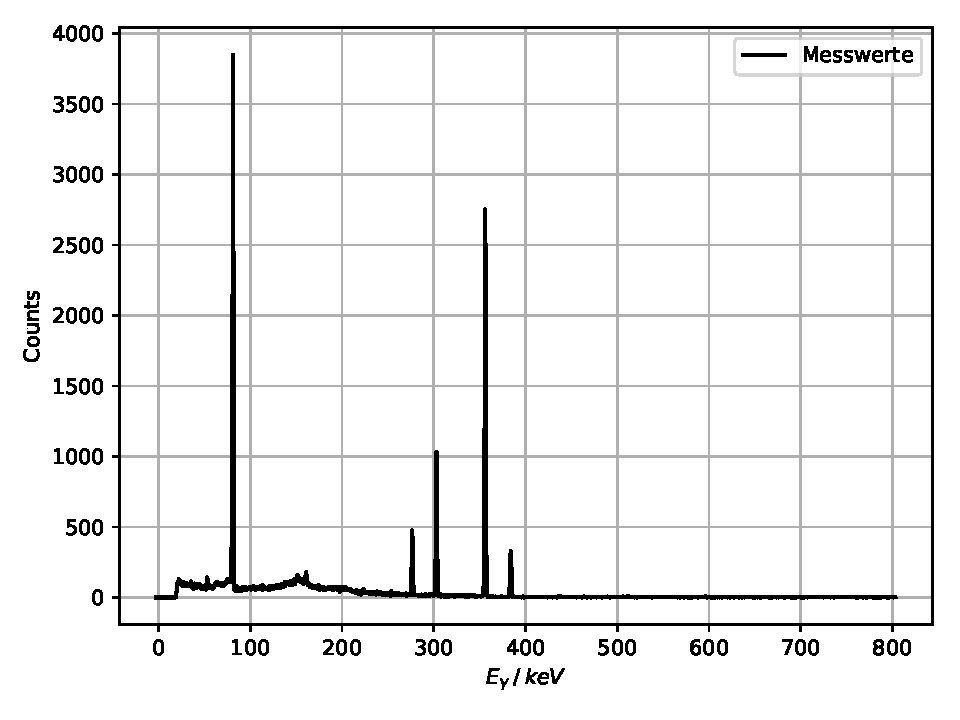
\includegraphics[height=9cm]{Ba.pdf}
  \caption{Unbekanntes Spektrum}
  \label{fig:plot7}
\end{figure}
Die Peaks werden erneut mit Gleichung \ref{eqn:gausk} gefittet und die resultierenden
Parameter in Tabelle \ref{tab:tabe5} dargestellt.
\begin{table}[H]
  \centering
  \caption{Bohrung 1 und 2, Vergleich der Sonden mit 1\;MHz und 2\;MHz.}
  \label{tab:tab5}
    \begin{tabular}{c c c c}
    \toprule
    Bohrung & $S_{\text{2\;MHz}}$/\;mm & $S_{\text{ 1\;MHz}}$/\;mm\\
    \midrule
    1 & 1,82 & 2,12\\
    2 & 1,83 & 1,97\\
    \bottomrule
    \end{tabular}
  \end{table}

Durch einen Vergleich mit der Datenbank
\cite{Lara} fällt auf, dass die Peaks mit denen von Barium übereinstimmen und es sich somit
bei der Probe offensichtlich um Barium handelt. Die Zuordnung zu den theoretischen Emissionslinien
und die entsprechenden Absorptionswahrscheinlickeiten sind in Tabelle \ref{tab:tabe6} angegeben.
\begin{table}[H]
  \centering
  \caption{Werte der Anpassungsschicht}
  \label{tab:tabe6}
    \begin{tabular}{S S S }
    \toprule
    $ \text{Zylinder} $ & $ \increment t [\mu\text{s}] $ &
    $ l_a \text{[mm]}$\\
    \midrule
    1 & 0.54 & 0.81 \\
    2 & 0.40 & 0.59 \\
    3 & 0.76 & 1.12 \\
    \text{1+2} & 0.49 & 0.73 \\
    4 & 0.70 & 1.03 \\
    \text{1+3} & 0.90 & 1.33 \\
    5 & 1.25 & 1.85 \\
    \text{1+4} & 0.69 & 1.02 \\
    6 & 0.44 & 0.66 \\

          \bottomrule
    \end{tabular}
  \end{table}

Zur Bestimmung der Aktivität wird mittels Gleichung \ref{eqn:inh} zunächst der Inhalt der Peaks errechnet.
Aus Gleichung \ref{eqn:itheo} lässt sich ein linearer Zusammenhang zwischen diesem Inhalt und der Aktivität
erkennen, wobei der Proportionalitätsfaktor durch
\begin{equation}
  l = P\cdot \frac{\Omega}{4\pi}\cdot t \cdot Q
  \label{eqn:lin}
\end{equation}
gegeben ist. Zur Bestimmung der Aktivität wird also eine Lineare Ausgleichsrechnung
gemäß Formel \ref{eqn:li} mit Wertepaaren aus $l$ und $\symup{I}$ durchgeführt,
wobei der Fitparameter a die Aktivität angibt. Dabei wird die $\SI{81.0657}{\kilo\electronvolt}$
außer Acht gelassen, da bei so niedrigen Energien der Quotient $Q$ der Vollenergienachweiswahrscheinlichkeit
zu ungenau ist. Somit ergeben sich die Parameter
\begin{align*}
  a = 416.4 \pm 2.7 \\
  b = 35 \pm 14
\end{align*}
und damit eine Aktivität von $\SI{416.4(27)}{\becquerel} $.
Die Wertepaare und die Ausgleichsgerade sind in Abbildung \ref{fig:plot9} dargestellt.
\begin{figure}
  \centering
  \includegraphics[height=9cm]{Plot9.pdf}
  \caption{Lineare Regression zur Aktivitätsbestimmung von $\ce{^{133}Ba}$}
  \label{fig:plot9}
\end{figure}



\subsection{Nuklididentikation}
Im letzten Versuchsteil wird eine Probe unbekannter Zusammensetzung untersucht, wobei die
Messzeit $\SI{4064}{\second}$ beträgt. Von den 8191 gemessenen Kanälen werden die ersten 6000 zur Auswertung
verwendet, die entsprechenden Messwerte werden gemäß Gleichung \ref{eqn:gerade} kalibriert und
sind in Abbildung \ref{fig:plot8} dargestellt.
\begin{figure}
  \centering
  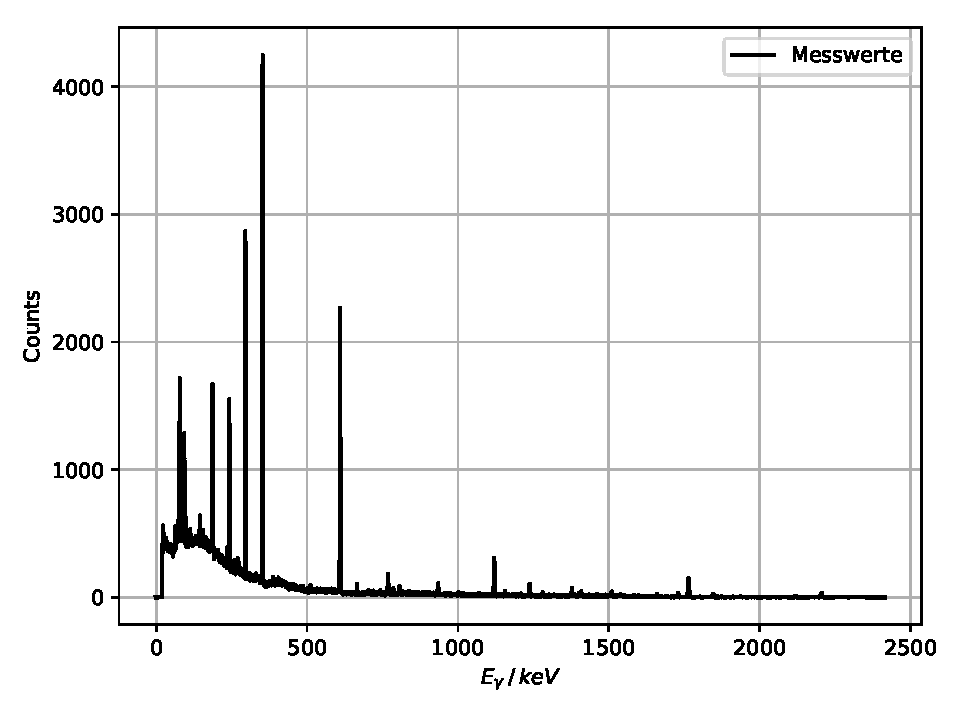
\includegraphics[height=9cm]{Un.pdf}
  \caption{Unbekanntes Spektrum}
  \label{fig:plot8}
\end{figure}

Um die Energie der Peaks zu bestimmen und sie somit zuordnen zu können, werden sie
wieder an die Gaußkurve gemäß Gleichung \ref{eqn:gausk} angepasst. Die Fitparameter sind in Tabelle
\ref{tab:tabe7} angegeben.

\begin{table}[H]
  \centering
  \caption{Parameter der gefitteten Gaußkurven}
  \label{tab:tabe7}
    \begin{tabular}{l l l l}
    \toprule
    $ a $ & $ b $ & $ c $
    & $ z \:/ \:\si{\kilo\electronvolt} $ \\
    \midrule
    593 \pm 23 & 1156 \pm 143 & 0.573 \pm 0.083 & 77.124 \pm 0.058 \\
    556 \pm 17 & 769 \pm 104 & 0.603 \pm 0.095 & 92.632 \pm 0.066 \\
    375.6 \pm 4.9 & 1335 \pm 25 & 0.772 \pm 0.017 & 186.090 \pm 0.012 \\
    252.8 \pm 6.2 & 1308 \pm 33 & 0.719 \pm 0.022 & 242.066 \pm 0.015 \\
    179.7 \pm 2.7 & 2711 \pm 14 & 0.7850 \pm 0.0048 & 295.3181 \pm 0.0033 \\
    130.2 \pm 4.2 & 4164 \pm 21 & 0.8586 \pm 0.0050 & 352.0054 \pm 0.0034 \\
    46.7 \pm 3.0 & 2230 \pm 12 & 1.1737 \pm 0.0076 & 609.2939 \pm 0.0052 \\
    31.3 \pm 1.1 & 64.9 \pm 4.2 & 1.33 \pm 0.10 & 665.409 \pm 0.070 \\
    31.3 \pm 1.3 & 158.5 \pm 4.6 & 1.451 \pm 0.051 & 768.246 \pm 0.034 \\
    30.9 \pm 1.0 & 38.9 \pm 3.9 & 1.29 \pm 0.16 & 785.87 \pm 0.10 \\
    30.7 \pm 1.0 & 46.6 \pm 4.1 & 1.20 \pm 0.13 & 806.244 \pm 0.085 \\
    26.3 \pm 1.1 & 72.9 \pm 3.7 & 1.68 \pm 0.10 & 934.015 \pm 0.067 \\
    18.2 \pm 1.9 & 292.3 \pm 5.8 & 1.782 \pm 0.043 & 1120.275 \pm 0.028 \\
    16.44 \pm 0.76 & 32.8 \pm 2.3 & 1.87 \pm 0.16  & 1155.44 \pm 0.10 \\
    13.1 \pm 1.1 & 98.2 \pm 3.1 & 2.037 \pm 0.078 & 1238.098 \pm 0.051 \\
    16.17 \pm 0.93 & 55.9 \pm 2.7 & 1.91 \pm 0.11 & 1377.862 \pm 0.074 \\
    17.5 \pm 1.3 & 25.6 \pm 3.8 & 1.95 \pm 0.36 & 1408.31 \pm 0.23 \\
    13.89 \pm 0.95 & 19.6 \pm 2.4 & 2.33 \pm 0.36 & 1509.44 \pm 0.22 \\
    4.78 \pm 0.63 & 12.2 \pm 1.3 & 2.96 \pm 0.40 & 1661.07 \pm 0.24 \\
    3.029 \pm 0.73 & 28.2 \pm 1.6 & 2.75 \pm 0.20 & 1729.76 \pm 0.12 \\
    3.0 \pm 1.79 & 145.9 \pm 3.9 & 2.725 \pm 0.093 & 1764.689 \pm 0.057 \\
    3.56 \pm 0.78 & 20.2 \pm 1.7 & 2.77 \pm 0.29 & 1847.40 \pm 0.18 \\
    0.71 \pm 0.87 & 29.1 \pm 1.6 & 3.35 \pm 0.24 & 2204.71 \pm 0.13 \\



          \bottomrule

    \end{tabular}
\end{table}

Die Linienenergien werden dann mit der Datenbank \cite{lara} abgeglichen und
passenden Nukliden zugeordent.
Diese Zuordnung ist in Tabelle \ref{tab:tabe8} zusammen mit den jeweiligen Emissionswahrscheinlichkeiten
dargestellt.
\begin{table}[H]
  \centering
  \caption{Werte der Messreihe die Wien-Robinson-brücke}
  \label{tab:tabe8}
    \begin{tabular}{c c c c}
    \toprule
    $ \nu \: / \: \si{\hertz} $ & $\text{U}_b \: / \: \si{\volt} $ &
    $\text{U}_s \: / \: \si{\volt} $ &
    $\frac{U_b}{U_s}$ \\
    \midrule
    20 & 0.120 & 3.08 & 0.039 \\
    50 & 0.248 & 4.56 & 0.054 \\
    100 & 0.320 & 4.64 & 0.069 \\
    150 & 0.264 & 4.56 & 0.058 \\
    200 & 0.136 & 4.50 & 0.030 \\
    220 & 0.072 & 4.48 & 0.016 \\
    230 & 0.032 & 4.48 & 0.007 \\
    240 & 0.024 & 4.48 & 0.005 \\
    242 & 0.016 & 4.48 & 0.004 \\
    250 & 0.040 & 4.48 & 0.009 \\
    265 & 0.080 & 4.48 & 0.018 \\
    300 & 0.298 & 4.56 & 0.065 \\
    500 & 0.704 & 4.56 & 0.154 \\
    1000 & 1.17 & 4.32 & 0.271 \\
    3000 & 1.41 & 4.28 & 0.330 \\
    10000 & 1.44 & 4.24 & 0.340 \\
    20000 & 1.44 & 4.24 & 0.340 \\
    30000 & 1.44 & 4.24 & 0.340 \\

    \bottomrule
    \end{tabular}
\end{table}

Alle identifizierten Nuklide gehören zu der Uran-Radium Zerfallsreihe, welche auch als 4n+2
Reihe bekannt ist. Es lässt sich also vermuten, dass die Probe ursprünglich zum Teil aus
$\ce{^{238}U}$ oder $\ce{^{234}Th}$ bestand, welches über  die Zeit zerfallen ist und somit die
radioaktiven Tochternuklide $\ce{^{226}Ra}$, $\ce{^{214}Pb}$ und $\ce{^{214}Bi}$ erklärt.
Alle weiteren Nuklide der Reihe haben keine, oder zumindest nur sehr schwache
Gammasignaturen, sodass diese nicht detektiert werden können.
Für die Aktivitätsbestimmung sind nur bei $\ce{^{214}Pb}$ und $\ce{^{214}Bi}$ genügend
Linien vorhanden um eine nicht allzu ungenaue Rechnung durchführen zu können. Das Vorgehen ist analog zur
Bestimmung der Aktivität von $\ce{^{133}Ba}$ und die resultierenden Ausgleichsgeraden sind in den
Abbildungen \ref{fig:plot11} und \ref{fig:plot12} dargestellt. Bei der Aktivitätsbestimmung
von $\ce{^{214}Pb}$ wurde die $\SI{77.1088}{\kilo\electronvolt}$ Linie außer acht gelassen,
da hier der Quotient $Q$ zu ungenau ist.
Es ergeben sich die Fitparameter
\begin{align*}
  a_{\text{Pb}} &= 1106 \pm 17 \\
  b_{\text{Pb}} &= -6\pm 69 \\
  a_{\text{Bi}} &= 1442 \pm 89 \\
  b_{\text{Bi}} &= 7 \pm 21 \\
\end{align*}
und somit Aktivitäten von $\SI{1106(17)}{\becquerel} $ für $\ce{^{214}Pb}$ und
$\SI{1442(89)}{\becquerel} $ für $\ce{^{214}Bi}$.
\begin{figure}
  \centering
  \includegraphics[height=9cm]{Plot11.pdf}
  \caption{Lineare Regression zur Aktivitätsbestimmung von $\ce{^{214}Pb}$}
  \label{fig:plot11}
\end{figure}
\begin{figure}
  \centering
  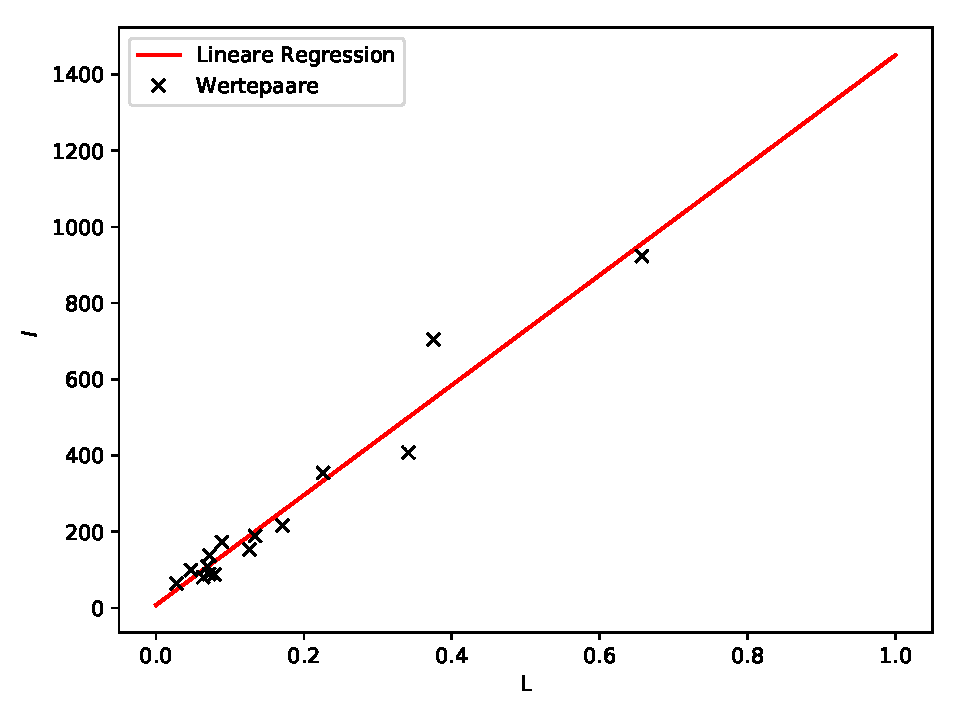
\includegraphics[height=9cm]{plot12.pdf}
  \caption{Lineare Regression zur Aktivitätsbestimmung von $\ce{^{214}Bi}$}
  \label{fig:plot12}
\end{figure}

\section{Diskussion}
Die lineare Regression zur Bestimmung der Energiekalibration liefert sehr geringe Ungenauigkeiten
der Fitparameter und scheint somit sehr exakt zu sein, was für ein gutes Auflösungsvermögen
des Detektors spricht. Die Parameter des Fits für die Vollenergienachweiswahrscheinlichkeit sind hingegen
mit einem großen relativen Fehler behaftet, welche teilweise sogar größer als der
eigentliche Wert sind. Dies lässt darauf schließen, dass eine Potenzfunktion
nicht vollständig zur Beschreibung der Energieabhängigkeit geeignet ist und
eine andere Funktion eventuell besser zu den Daten passen würde. \\
Die Abweichung in der gemessenen Energie des $\ce{^{137}Cs}$-Strahlers beträgt lediglich
0.0088\%, wodurch erneut die gute Energieauflösung gezeigt wird. Wie bereits erwähnt
ist die Beschreibung der Peaks durch Gaußkurve sehr genau und weißt im Verhältniss
von Halb- und Zehntelwertsbreite nur eine Abweichung von 1.64 \% auf. \\
Auch die Componkante und das Comptonkontinuum können recht genau bestimmt werden,
jedoch ergibt sich bei dem Rückstreupeak eine Abweichung von 5,14 \% , wobei der Theoriewert etwa 39,44
Fehlerintervalle von dem experimentellen Wert abweicht. Es wird somit vermutlich ein systematischer Fehler
vorliegen. \\
Auch bei dem Verhältniss des Inhalts von Comptonkontinuum und Photopeak gibt es eine
sehr große Abweichung, was vermutlich daran liegt, dass Mehrfachstreuung beim
Comptoneffekt in den theoretischen Formeln nicht berücksichtigt wird. Durch diese
Mehrfachstreuung deponiert die Gammastrahlung einen größeren Anteil oder eventuell auch die
gesamte Energie in dem Detektor, sodass der Inhalt des Comptonkontinuums sinkt und der
Inhalt des Photopeaks steigt, was den Betrag des Verhältnisses ansteigen lässt. \\
Die Aktivität lässt sich ebenfalls bis auf einen geringen
relativen Fehler bestimmen und auch die Zuordnung der Proben ist aufgrund der
guten Energieauflösung problemlos möglich. Lediglich die $\SI{92.38(1)}{\kilo\electronvolt}$-Linie
und die $\SI{92.80(1)}{\kilo\electronvolt}$-Linie von $\ce{^{234}Th}$ können nicht
getrennt aufgelöst werden, sondern erscheinen als ein einzelner Peak. Hier liegt offensichtlich
die Grenze des Auflösungsvermögens.


\printbibliography{}

\end{document}
||||||| merged common ancestors
\documentclass[
  bibliography=totoc,     % Literatur im Inhaltsverzeichnis
  captions=tableheading,  % Tabellenüberschriften
  titlepage=firstiscover, % Titelseite ist Deckblatt
]{scrartcl}

% Paket float verbessern
\usepackage{scrhack}

% Warnung, falls nochmal kompiliert werden muss
\usepackage[aux]{rerunfilecheck}

% unverzichtbare Mathe-Befehle
\usepackage{amsmath}
% viele Mathe-Symbole
\usepackage{amssymb}
% Erweiterungen für amsmath
\usepackage{mathtools}

% Fonteinstellungen
\usepackage{fontspec}
% Latin Modern Fonts werden automatisch geladen
% Alternativ zum Beispiel:
%\setromanfont{Libertinus Serif}
%\setsansfont{Libertinus Sans}
%\setmonofont{Libertinus Mono}

% Wenn man andere Schriftarten gesetzt hat,
% sollte man das Seiten-Layout neu berechnen lassen
\recalctypearea{}

% deutsche Spracheinstellungen
\usepackage{polyglossia}
\setmainlanguage{german}


\usepackage[
  math-style=ISO,    % ┐
  bold-style=ISO,    % │
  sans-style=italic, % │ ISO-Standard folgen
  nabla=upright,     % │
  partial=upright,   % ┘
  warnings-off={           % ┐
    mathtools-colon,       % │ unnötige Warnungen ausschalten
    mathtools-overbracket, % │
  },                       % ┘
]{unicode-math}

% traditionelle Fonts für Mathematik
\setmathfont{Latin Modern Math}
% Alternativ zum Beispiel:
%\setmathfont{Libertinus Math}

\setmathfont{XITS Math}[range={scr, bfscr}]
\setmathfont{XITS Math}[range={cal, bfcal}, StylisticSet=1]

% Zahlen und Einheiten
\usepackage[
  locale=DE,                   % deutsche Einstellungen
  separate-uncertainty=true,   % immer Fehler mit \pm
  per-mode=symbol-or-fraction, % / in inline math, fraction in display math
]{siunitx}

% chemische Formeln
\usepackage[
  version=4,
  math-greek=default, % ┐ mit unicode-math zusammenarbeiten
  text-greek=default, % ┘
]{mhchem}

% richtige Anführungszeichen
\usepackage[autostyle]{csquotes}

% schöne Brüche im Text
\usepackage{xfrac}

% Standardplatzierung für Floats einstellen
\usepackage{float}
\floatplacement{figure}{htbp}
\floatplacement{table}{htbp}

% Floats innerhalb einer Section halten
\usepackage[
  section, % Floats innerhalb der Section halten
  below,   % unterhalb der Section aber auf der selben Seite ist ok
]{placeins}

% Seite drehen für breite Tabellen: landscape Umgebung
\usepackage{pdflscape}

% Captions schöner machen.
\usepackage[
  labelfont=bf,        % Tabelle x: Abbildung y: ist jetzt fett
  font=small,          % Schrift etwas kleiner als Dokument
  width=0.9\textwidth, % maximale Breite einer Caption schmaler
]{caption}
% subfigure, subtable, subref
\usepackage{subcaption}

% Grafiken können eingebunden werden
\usepackage{graphicx}
% größere Variation von Dateinamen möglich
\usepackage{grffile}

% schöne Tabellen
\usepackage{booktabs}

% Verbesserungen am Schriftbild
\usepackage{microtype}

% Literaturverzeichnis
\usepackage[
  backend=biber,
]{biblatex}
% Quellendatenbank
\addbibresource{lit.bib}
\addbibresource{programme.bib}

% Hyperlinks im Dokument
\usepackage[
  unicode,        % Unicode in PDF-Attributen erlauben
  pdfusetitle,    % Titel, Autoren und Datum als PDF-Attribute
  pdfcreator={},  % ┐ PDF-Attribute säubern
  pdfproducer={}, % ┘
]{hyperref}
% erweiterte Bookmarks im PDF
\usepackage{bookmark}

% Trennung von Wörtern mit Strichen
\usepackage[shortcuts]{extdash}

\author{%
  AUTOR A\\%
  \href{mailto:authorA@udo.edu}{authorA@udo.edu}%
  \texorpdfstring{\and}{,}%
  AUTOR B\\%
  \href{mailto:authorB@udo.edu}{authorB@udo.edu}%
}
\publishers{TU Dortmund – Fakultät Physik}


\subject{Versuch 351}
\title{Fourier- Analyse und Sythese}
\date{%
  Durchführung: 14.11.2018
  \hspace{3em}
  Abgabe: 21.11.2018
}

\begin{document}

\maketitle
\thispagestyle{empty}
\tableofcontents
\newpage

\section{Zielsetzung}
Ziel ist es für eine unbekannte Probe die aktiven Isotope und deren Aktivität zu ermitteln,
dafür ist es zuvor notwendig mit bekannten Elementen die Detektoreigenschaften
zu bestimmen.

\section{Theorie}
\subsection{Wechselwirkung von Strahlung mit Materie}
Wechselwirkt Strahlung mit Materie, so wird die Intensität der Strahlung durch das Material
abgeschwächt, diese Intensitätsabnahme kann allgemein über das Lambert-Beersche-Gesetz beschrieben werden:
\begin{equation}
  I(x)=I_0\cdot\exp(-\mu x).
  \label{eqn:lambert}
\end{equation}
Dabei bezeichnet $\mu$ den Extinktionskoeffizienten oder auch Abschwächungskoeffizient genannt, dieser
setzt sich aus Absorption und Streuung zusammen und lässt sich durch die Formel
\begin{equation}
  \mu=Zn\sigma
\end{equation}
beschreiben. Z bezeichnet die Ordnungszahl des Materials, n die Teilchenzahldichte und $\sigma$ den
Wirkungsquerschnitt der sich aus den verschiedenen Wechselwirkungen zusammensetzt.
\begin{figure}[H]
  \centering
  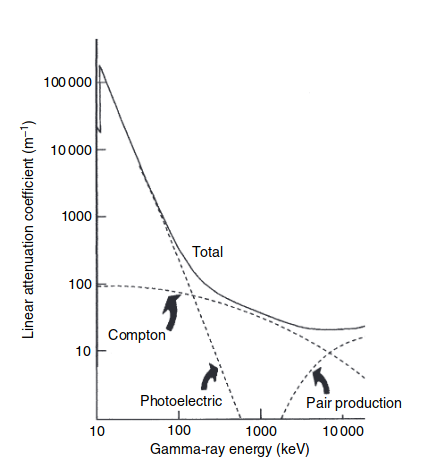
\includegraphics[height=8cm]{Extin.png}
  \caption{Der Extinkionskoeffizient in Abhängigkeit der Energie für verschiedene Prozesse. \cite{Gilmore2}}
  \label{fig:Extin}
\end{figure}

Wie in Abbildung \ref{fig:Extin} zu sehen ist, dominieren bei verschiedenen Energien
unterschiedliche Prozesse. Für geringe Energien dominiert der Photoeffekt, welcher mit
steigender Energie abnimmt, dadurch gewinnt der Comptoneffekt an Bedeutung. Für hohe
Energien dominiert die Paarerzeugung.
Da diese drei Prozesse für die Wechselwirkung von Gammaquanten mit Materie von großer Bedeutung sind
werden sie im Folgenden näher betrachtet.
\cite{Springer3}
\\
\\
\textbf{1. Photoeffekt}\\
Ein Gammaquant wird von einem kernnahen Hüllenelektron (bevorzugt aus der K-Schale) absorbiert,
wodurch das Hüllenelektron ausgelöst wird. Voraussetzung für diesen Effekt ist, dass das Gammaquant
mindestens die Bindungsenergie des Elektrons besitzt, überschüssige Energie wird als kinetische
Energie an das Elektron übertragen.
Das so entstandene "Loch" in der Elektronenhülle wird durch ein energiereicheres Hüllenelektron
gefüllt welches bei dem Übergang aus einer höheren Schale in eine niedrigere Schale
charakteristische Röntgenstrahlung emittiert.
Da sowohl die Röntgenstrahlung als auch das ausgelöste Elektron im Detektor verbleiben und
dort detektiert werden, verbleibt beim Photoeffekt die gesamte Gammaenergie im Detektor, weshalb
der Photopeak besonders wichtig für die Gammaspektroskopie ist.
Der differentielle Wirkungsquerschnitt der Energie lässt sich über die Formel
\begin{equation}
  \frac{d \sigma}{d E} = \bigg(-\frac{64}{7E^{9}}\bigg)^{1/2}\alpha^4 Z^5\sigma_{Th}
  \label{eqn:diffPhoto}
\end{equation}
beschreiben, wobei $\sigma_{Th}$ den Thomson-Wirkungsquerschnitt $\sigma_{Th} = \frac{8}{3}\pi r_{e}^2$
beschreibt mit $r_e$ als klassischen Elektronenradius.
(Thomson-Streuung: Streuung niederenergetischer Photonen an Elektronen) \cite{Springer3}
Der totale Wirkungsquerschnitt für den Photoeffekt ist von der Ordnungszahl des Materials
und der Photonenergie abhängig:
\begin{equation}
  \sigma_{\text{Photo}}\sim Z^5\cdot E_{\gamma}^{-7/2}.
  \label{eqn:WQphoto}
\end{equation}
\cite{Karlsruhe}
\\
\\

\textbf{2. Comptoneffekt}\\
Der Comptoneffekt beschreibt die Streuung von Photonen an äußeren Hüllenelektronen. Da
diese Streuung sehr stark winkelabhängig ist, kann von der gemessenen Elektronenenergie
nicht auf die Energie des Gammaquants geschlossen werden wodurch sich ein kontinuierliches
Spektrum, das Comptonkontinuum bildet. Dieses Spektrum bricht an der Comptonkante ab, hier
beträgt der Streuwinkel 180° und der Energieübertrag $E_{\text{max}}$ ist maximal, trotzdem gibt das
Gammaquant nicht seine gesamte Energie ab
\begin{equation}
  E_{max}=E_{\gamma}\cdot\frac{2\epsilon}{1+2\epsilon}\;\;<E_{\gamma}.
  \label{eqn:kante}
\end{equation}
\cite[Springer3]
Hier ist der Wirkungsquerschnitt über die Klein-Nishina-Formel gegeben, aus dieser ergibt sich der
differentielle Wirkungsquerschnitt:
\begin{equation}
  \frac{d\sigma}{dE}=\frac{3}{8}\sigma_{\text{Th}}\frac{1}{m_0 c^2 e^2}\bigg(2+\bigg(\frac{E}{h\nu-E} \bigg)^2 \bigg[\frac{1}{\epsilon^2}+
  \frac{h\nu-E}{h\nu}-\frac{2}{\epsilon}\bigg(\frac{h\nu-E}{h\nu}\bigg) \bigg]\bigg)
  \label{eqn:diffCompton}
\end{equation}
mit $\epsilon=\sfrac{E_{\gamma}}{m_e c^2}$.
Für den totalen Wirkungsquerschnitt gilt der Zusammenhang
\begin{equation}
  \sigma_{\text{Compton}}\sim \frac{Z}{E_{\gamma}}.
  \label{eqn:WPCompton}
\end{equation}
\\
\\
\textbf{3. Paarerzeugung}\\
Sind die Photonen energiereich genug können Elektron-Positron-Paare erzeugt werden, dafür müssen
die Photonen eine Mindestenergie von $E=2 m_0 c^2$ besitzen, also die doppelte
Ruheenergie des Elektrons.
Das so entstandene Positron annihiliert mit den im Detektor vorhandenen Elektronen und es
entstehen zwei Photonen. Wenn beide Photonen den Detektor verlassen wird dies als double-escape
bezeichnet, verlässt nur eins den Detektor entsteht der single-escape Peak.
Der differentielle Wirkungsquerschnitt für den Prozess der Paarerzeugung ist durch
\begin{equation}
  \frac{d\sigma}{dE}= \frac{28\alpha Z^2 r_{e}^2}{9E_{\gamma}}
  \label{eqn:diffPaar}
\end{equation}
gegeben, während der totale Wirkungsquerschnitt folgende Proportionalität besitzt:
\begin{equation}
  \sigma_{\text{Paar}}\sim Z^2\cdot\ln\Bigg(\frac{2E_{\gamma}}{m_e c^2}\Bigg).
  \label{eqn:WQPaar}
\end{equation}
\\

Eine Übersicht über die möglichen Wechselwirkungen von Gammaquanten mit Materie liefert
Abbildung \ref{fig:Effekt}.
\begin{figure}[H]
  \centering
  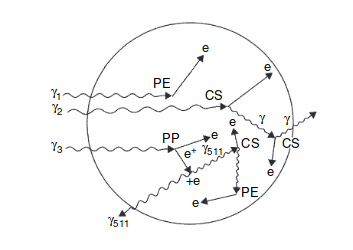
\includegraphics[height=5cm]{Effekte.png}
  \caption{Übersicht der Prozesse im Detektor. \cite{Gilmore2}}
  \label{fig:Effekt}
\end{figure}


\subsection{Grundlagen der Halbleiterinstrumente}
Halbleiter werden zwischen direkten und indirekten Halbleitern unterschieden, dies wird
in Abbildung \ref{fig:Band} dargestellt. Bei direkten Halbleitern
liegt das Maximum des Valenzbands genau unter dem Minimum des Leitungsbandes, somit ist ein direkter Bandübergang möglich.
Bei indirekten Halbleitern liegen Minima und Maxima nicht übereinander, für diesen indirekten Bandübergang ist
ein weiteres Photon nötig.\\

\begin{figure}
  \centering
  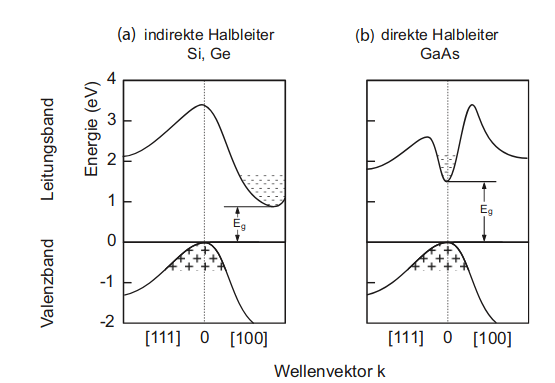
\includegraphics[height=6cm]{Band.png}
  \caption{Bandstruktur für direkte und indirekte Halbleiter.}
  \label{fig:Band}
  \cite{Springer3}
\end{figure}

Außerdem werden die Eigenschaften von Halbleitern durch ihre Dotierung beeinflusst. Germanium besitzt
beispielsweise 4 Valenzelektronen, wird nun ein Material mit fünf Valenzelektronen hinzugegeben bleibt nach
Eingehen der Bindungen ein freies Elektron übrig, somit dominieren die Elektronen als Ladungsträger und es handelt
sich um einen n-dotierten Halbleiter.
Wird stattdessen ein dreiwertiges Element verwendet bleibt ein Loch, somit stehen die Löcher als
positive Ladungsträger zur Verfügung und es handelt sich um einen p-dotierten Halbleiter.\\

\begin{figure}[H]
  \centering
  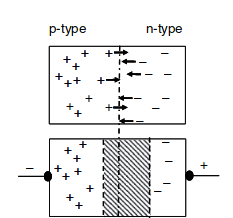
\includegraphics[height=6cm]{pn.png}
  \caption{Bildung einer Verarmungsschicht im pn-Übergang und Verbreiterung dieser durch
  anlegen einer äußeren Spannung.}
  \label{fig:pn}
  \cite{Gilmore2}
\end{figure}

Wie in Abbildung \ref{fig:pn} gezeigt entsteht ein pn-Übergang wenn p- und n-dotierte Halbleiter zusammengebracht werden,
Elektronen und Löcher vernichten sich in einem Teilbereich wodurch eine Verarmungszone entsteht.
Durch anlegen einer äußeren Spannung kann die Größe der Verarmungszone verändert werden. Für die
Verwendung als Detektor ist eine große Verarmungszone gewünscht, da dieser Bereich den
Detektorbereich bildet, also wird die Spannung in Sperrrichtung angelegt.


\subsection{Der Halbleiterdetektor}
Bei dem verwendeten Detektor handelt es sich um einen koaxialen Ge-Detektor wie in Abbildung
\ref{fig:Aufbau} zu sehen ist. Der gesamte Detektor befindet sich unter einer Aluminium
Schutzhaube und ist von außen mit Li-Atomen n-dotiert, wodurch die Oberfläche
gut leitend wird. Im Inneren befindet sich eine Bohrung, diese innere Oberfläche ist
mit Au-Atomen p-dotiert. (Die Dotierung ist hier etwas anders als oben beschrieben, da es sich um
Metall-Halbleiterkontakte handelt.) An diese dotierten Schichten wird die
äußere Spannung angelegt, die n-dotierte Schicht dient als Anschluss für den Pluspol.
Durch die p- und n-dotierten Bereiche bildet sich eine
Verarmungszone im Detektor die den Detektorbereich bildet. Somit müssen die Gammaquanten erst
die Al-Schicht und die Li-Schicht durchdringen um detektiert zu werden, dadurch kommt es zu einer
unteren Nachweisenergie der Gammaenergie, diese liegt bei 40 bis 50\;keV.
Dieser Gesamte Aufbau, wie in Abbildung \ref{fig:Aufbau} gezeigt befindet sich in einem
Bleigehäuse welches von innen mit Kupferplatten ausgelegt ist. Das Bleigehäuse dient zur Abschiermung
äußerer Strahlung, während die Kupferplatten die aus dem Blei austretende Strahlung
abhalten sollen.

\begin{figure}
  \centering
  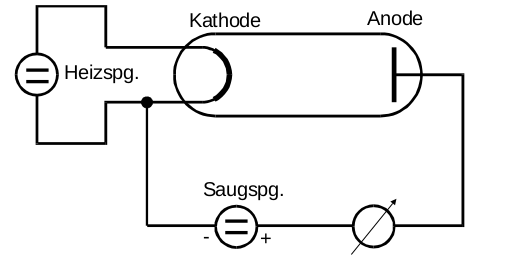
\includegraphics[height=7cm]{Aufbau.png}
  \caption{Schematischer Aufbau des Ge-Detektors. \cite{skript}}
  \label{fig:Aufbau}
\end{figure}

Dringt ein Gammaquant in die Verarmungszone ein wechselwirkt es mit der Materie und kann
z.B. ein Elektron auslösen welches mit anderen Elektronen stößt und ein Elektronen-Loch-Paar erzeugt.
Durch die angelegte Spannung wird das Paar räumlich getrennt wodurch eine Rekombination verhindert wird,
der dadurch entstehende Ladungsimpuls
wird verstärkt und bildet das Detektorsignal. Dieses ist proportional zu der einfallenden Photonenergie, da mit
einer höheren Energie auch mehr Elektronen-Loch-Paare erzeugt werden können.
Dringt das Gammaquant außerhalb der Verarmungszone in den Detektor ein rekombinieren die
Elektronen-Loch-Paare sofort, somit kann kein Signal gemessen werden.\\
Um Störsignale zu minimieren wird der Detektor mit Stickstoff auf 77\;K gekühlt, denn durch die
hohe externe Spannung kommt es zu thermischen Effekten wodurch sich noch Ladungsträger in der Verarmungszone
befinden und das Signal stören können.
\\
\\
\textbf{Eigenschaften eines Halbleiterdetektors}\\
Eine charakteristische Größe des Detektors ist das Auflösungsvermögen, dieses wird durch die
Halbwertsbreite $\Delta E_{1/2}$ der Impulshöhenverteilung beschrieben. Energien mit den Mittelwerten
$E_1$ und $E_2$ können noch voneinander unterschieden werden, wenn der Energieunterschied mindestens
$\Delta E_{1/2}$ beträgt.

Die Vollenergienachweiswahrscheinlichkeit eines Detektors gibt die Nachweiswahrscheinlichkeit eines Detektors
in Abhängigkeit der Energie an. Um sie zu bestimmen wird aus der aktuellen Aktivität der Probe der
theoretische Linieninhalt bestimmt, der Quotient aus gemessenem Linieninhalt und theoretischem
Linieninhalt gibt die Nachweiswahrscheinlichkeit des Detektors an.

\subsection{Das Spektrum eines monochromatischen Gammastrahlers}
Das Spektrum eines monochromatischen Gammastrahlers zeigt mehrere Besonderheiten auf, wie in Abbildung \ref{fig:Spektrum} zu
sehen. Wesentliche Bestandteile sind das Comptonkontinuum mit der Comptonkante, der Rückstreupeak
und der Photopeak. Der Photopeak entsteht dadurch, dass die Gammaquanten ihre gesamte Energie im Detektor deponieren
und wird daher auch Vollenergiepeak genannt. Er entsteht wenn die Gammaquanten im Detektor durch
Comptonstreuung genügend Energie verlieren bis der Photoeffekt eintreten kann und die restliche Energie
an den Detektor abgegeben wird. Auf diese Weise deponieren die Gammaquanten ihre gesamte Energie im
Detektor, so dass das Maximum des Photopeaks die Energie der Gammastrahlung angibt.\\
Das Comptonkontinuum entsteht durch Comptonstreuung der Gammaquanten, erfolgt die Streuung im
180° Winkel wobei der Energieübertrag maximal ist entsteht die Comptonkante. Da durch mehrfache
Comptonstreuung ein größerer Energieübertrag möglich ist als duch eine einmalige Streuung im 180° Winkel ist die
Componkante ausgeschmiert.\\
Da die Strahlung der Probe keine Vorzugsrichtung hat, wechselwirken einige Gammaquanten auch mit der
Abschirmung des Detektors und verlieren so Energie, werden sie dann so zurückgestreut, dass sie den
Detektor erreichen bilden sie den Rückstreupeak, dieser liegt bei
\begin{equation}
  E_{\text{Rück}}=E_{\gamma}\frac{1}{1+2\epsilon}
  \label{eqn:Rückstreu}
\end{equation}
Zwei weitere mögliche Peaks sind double- und single-escape Peak. Fällt ein Gammaquant in den Detektor und wechselwirkt über
Paarerzeugung entsteht ein Elektron und ein Positron, das Positron annihiliert mit den Elektronen der umgebenden Materie wobei
zwei Photonen erzeugt werden. Verlässt eins dieser Photonen den Detektor komm es zu single-escape Peak, verlassen beide
Photonen den Detektor entsteht der double-escape Peak.
\cite{Gilmore2}


\begin{figure}
  \centering
  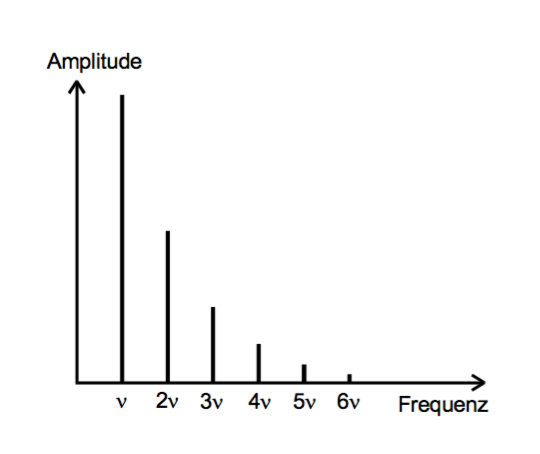
\includegraphics[height=7cm]{Spektrum.png}
  \caption{Gammaspektrum von $\ce{^{28}Al}$. Die Componkante ist hier nicht eingezeichnet, sie ist der Peak zwischen single escape und Photopeak,
  das Comptonkontinuum verläuft von der y-Achse bis zur Comptonkante.}\cite{Gilmore2}
  \label{fig:Spektrum}
\end{figure}

\section{Durchführung}
\label{sec:Durchführung}
Zunächst wird eine kalibrierte $\ce{^{152}Eu}$-Probe vermessen die später zur Energiekalibration
genutzt wird. Die Probe wird in die Probenhalterung des Detektors eingespannt, um für alle
Proben den gleichen Abstand zum Detektor zu garantieren wird ein Messingstab als Abstandshalter
verwendet, dieser wird vor der Messung natürlich wieder entfernt.
Auf dem Computer wird nun die Messung gestartet, die Messzeit beträgt ca. 3600\;s $\sim$ eine Stunde.\\
Für $\ce{^{137}Cs}$ und und eine weitere Probe (entweder $\ce{^{125}Sb}$ oder $\ce{^{133}Ba}$ )
wird äquivalent vorgegangen. Zuletzt wird eine unbekannte Probe vermessen, da diese eine andere
Form besitzt und nicht in den Probenhalter passt wird sie vor der Aluminiumschutzhaube des Detektors
platziert.

\section{Auswertung}
\label{sec:Auswertung}

\subsection{Energiekalibration und Bestimmung der Vollenergienachweiswahrscheinlichkeit}
Zur Kalibration wird ein $\ce{^{152}Eu}$-Strahler verwendet, dessen Aktivität am 01.10.2000
%\begin{align*}
%  \SI{4130(60)}{\becquerel}
%\end{align*}
$\SI{4130(60)}{\becquerel} $ betrug. \\
Nach dem Gesetz des radioaktiven Zerfalls berechnet sich die Aktivität am Messtag (08.04.2019) durch

\begin{equation}
  \symup{A} (t) = \symup{A}(0)\cdot \symup{e}^{-\lambda t} \: ,
\end{equation}

wobei $\lambda=\SI{1.6244(19)e-9}{\per\second}$ \cite{lara} die Zerfallskonstante
von $\ce{^{152}Eu}$ bezeichnet.

Der Fehler ergibt sich hierbei nach der Gauß´schen Fehlerfortpflanzung
\begin{equation}
  \increment f = \sqrt{ \sum_{i=1}^N \left( \frac{\partial f}{\partial x_i}\right)^2
  \cdot (\increment x_i)^2  } \: ,
  \label{eqn:gaus}
\end{equation}
also gemäß
\begin{equation}
  \increment \symup{A} (t) = \sqrt{ (\symup{e}^{-\lambda t})^{2}\cdot (\increment \symup{A}(0))^2
   + (-t\cdot\symup{A}(0)\cdot \symup{e}^{-\lambda t})^2\cdot(\increment \lambda)^2}
\end{equation}
Die Anzahl der Tage vom 01.10.2000 bis zum 08.04.2019 beträgt 6763 Tage, was
584323200 Sekunden entspricht, sodass sich insgesamt der Wert $\SI{1599(29)}{\becquerel} $
für die Aktivität der Probe am Messtag ergibt. \\
Der abgedeckte Raumwinkel lässt sich aus dem gemessenen Abstand a der Probe
zum Detektor, wobei auch der Abstand von $\SI{1.5}{\centi\meter}$ zwischen Al-Haube und Detektor
berücksichtigt wird,
und dem angegebenen Radius r des Detektorvolumens bestimmen. Die entsprechenden Werte
betragen
\begin{align*}
  a &= \SI{8.8}{\centi\meter} \\
  r &= \SI{2.25}{\centi\meter} \: .
\end{align*}

Die Formel zur Berechnung des abgedeckten Raumwinkelanteils ergibt sich dabei
über geometrische Überlegungen zu
\begin{equation}
  \frac{\Omega}{4\pi}= \frac{1}{2}(1-\frac{a}{\sqrt{a^2+r^2}})   \: ,
\end{equation}
in diesem Fall also $\frac{\Omega}{4\pi}= 0.01558$.
Diese somit errechneten Werte sind später wichtig zur Bestimmung der Vollenergienachweiswahrscheinlichkeit. \\
Das gemessene Spektrum des kalibrierten $\ce{^{152}Eu}$-Strahlers ist in Abbildung
\ref{fig:plot1} dargestellt. Es sind jedoch nur die ersten 4000 Kanäle dargestellt,
da bei höheren Kanälen keine signifikanten Messwerte mehr zu sehen sind. Die Messwerte
reichen bis Kanalnummer 8191 und die Messzeit beträgt $\SI{3598}{\second}$.
\begin{figure}
  \centering
  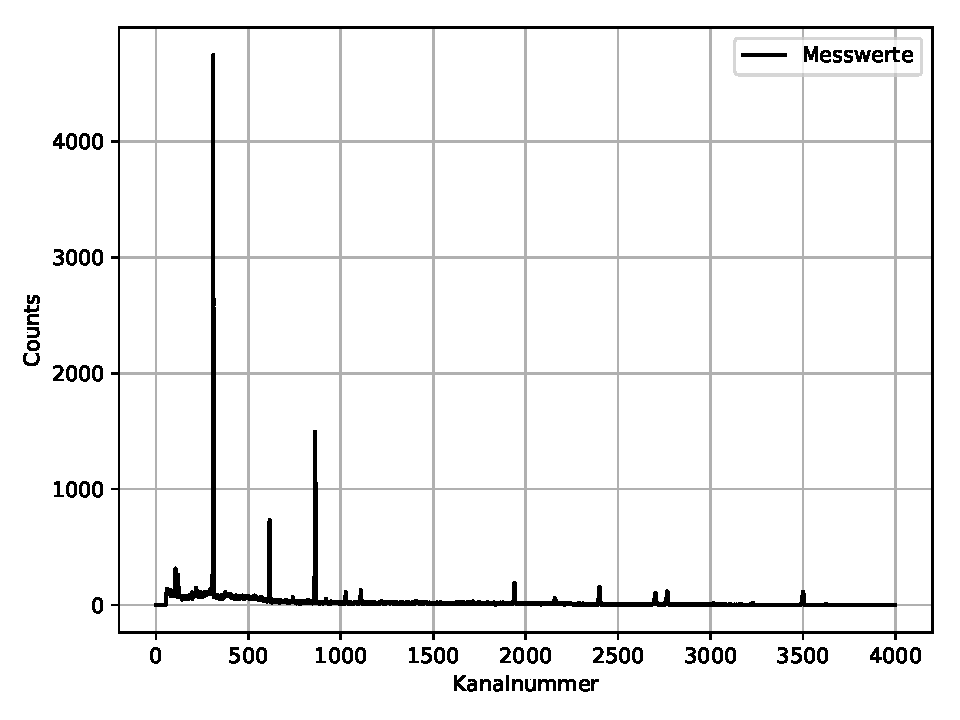
\includegraphics[height=9cm]{Eu.pdf}
  \caption{Spektrum des $\ce{^{152}Eu}$-Strahlers}
  \label{fig:plot1}
\end{figure}

Um mit diesem die Energiekalibration durchzuführen, werden die Peaks des Spektrums
jeweils mit einer Gaußverteilung der Form
\begin{equation}
  \symup{g} (x) = a + b \cdot \symup{e}^{(\frac{x-z}{c})^2}
  \label{eqn:gausk}
\end{equation}
gefittet.

Die sich daraus ergebenen Parameter sind in Tabelle \ref{tab:tabe1} angegebenen.
\begin{table}[H]
  \centering
  \caption{Messwerte der Wärmepumpe}
  \label{tab:tabe1}
    \begin{tabular}{S S S S S S}
    \toprule
    $ t  \: / \si{\second} $ & $ p_a \: / \si{\bar} $ & $ p_b \: / \si{\bar} $ &
    $ T_1 \: / \si{\kelvin} $ & $ T_2 \: / \si{\kelvin} $ & $ P \: / \: \si{\watt} $\\
    \midrule
    0 & 5.0 & 5.0 & 293.65 & 293.65 & 0 \\
    60 & 4.7 & 6.0 & 294.15 & 293.55 & 115 \\
    120 & 4.4 & 6.4 & 295.15 & 293.15 & 118 \\
    180 & 4.5 & 6.9 & 296.35 & 291.95 & 122 \\
    240 & 4.6 & 7.0 & 297.55 & 290.95 & 125 \\
    300 & 4.6 & 7.0 & 298.85 & 289.95 & 125 \\
    360 & 4.5 & 7.2 & 300.05 & 289.15 & 123 \\
    420 & 4.4 & 7.4 & 301.15 & 288.45 & 123 \\
    480 & 4.3 & 7.8 & 302.35 & 287.65 & 122 \\
    540 & 4.2 & 8.0 & 303.55 & 286.95 & 122 \\
    600 & 4.2 & 8.1 & 304.65 & 286.25 & 121 \\
    660 & 4.1 & 8.3 & 305.75 & 285.55 & 121 \\
    720 & 4.0 & 8.5 & 306.75 & 284.95 & 121 \\
    780 & 4.0 & 8.8 & 307.75 & 284.35 & 121 \\
    840 & 3.9 & 9.0 & 308.75 & 283.75 & 121 \\
    900 & 3.8 & 9.1 & 309.65 & 283.15 & 121 \\
    960 & 3.8 & 9.2 & 310.55 & 282.55 & 122 \\
    1020 & 3.8 & 9.5 & 311.45 & 282.05 & 122 \\
    1080 & 3.7 & 9.8 & 312.25 & 281.55 & 122 \\
    1140 & 3.7 & 10.0 & 313.05 & 281.15 & 122 \\
    1200 & 3.7 & 10.0 & 313.9 & 280.65 & 122 \\
    1260 & 3.6 & 10.2 & 314.65 & 280.25 & 123 \\
    1320 & 3.6 & 10.3 & 315.35 & 279.85 & 123 \\
    1380 & 3.6 & 10.6 & 316.15 & 279.45 & 124 \\
    1440 & 3.6 & 10.8 & 316.85 & 279.15 & 124 \\
    1500 & 3.6 & 11.0 & 317.55 & 278.75 & 124 \\
    1560 & 3.6 & 11.1 & 318.25 & 278.55 & 124 \\
    1620 & 3.6 & 11.2 & 318.95 & 278.25 & 125 \\
    1680 & 3.5 & 11.4 & 319.55 & 277.95 & 125 \\
    1740 & 3.5 & 11.5 & 320.15 & 277.65 & 125 \\
    1800 & 3.5 & 11.7 & 320.75 & 277.45 & 125 \\
    1860 & 3.5 & 11.9 & 321.35 & 277.25 & 125 \\
    1920 & 3.5 & 12.0 & 321.95 & 277.05 & 125 \\
    1980 & 3.5 & 12.1 & 322.45 & 276.95 & 125 \\








      \bottomrule
    \end{tabular}
\end{table}


Die zentrale Lage der Peaks im Hinblick auf die Kanalnummer ist durch den Parameter
z gegeben. Diese Werte werden zusammen mit der jeweiligen relativen Höhe mit den theoretischen
Emissionslinien der Datenbank \cite{lara} verglichen und es wird jedem Peak eine Linie
zugeordent. Diese Zuordnung ist zusammen mit der jeweiligen relativen Emissionswahrscheinlichkeit P
in Tabelle \ref{tab:tabe2} dargestellt.
\begin{table}[H]
  \centering
  \caption{Wertetabelle für $\alpha$ und $C_V$.}
  \label{tab:tab2}
    \begin{tabular}{S S S S S}
    \toprule
    $ T\: \text{in}\: \si{\K} $ & $ {\alpha \cdot 10^{-6} \: \text{in}\: \si {\per\K}} $ &
    $ C_V \: \text{in}\: \si{\J\per\K\mol} $\\
    \midrule %Cv, a *10-6, Cv
    %0 & 1 & 1\\
    88.60\pm0.24 & 9.56\pm0.06 & 14.17\pm8.13  \\ %&3.6 & 318.97\pm0.85\\
    93.81\pm0.24 & 10.10\pm0.06 & 17.58\pm10.03 \\ %& 4.7 & 440.90\pm1.11\\
    99.74\pm0.24 & 10.66\pm0.05 & 15.52\pm8.84 \\ %& 5.1 & 508.68\pm1.21\\
    104.74\pm0.24 & 11.07\pm0.05 & 18.44\pm10.52 \\ %& 4.6 & 481.79\pm1.09\\
    110.94\pm0.24 &  11.54\pm0.05 & 14.86\pm8.45 \\ %& 5.3 & 587.97\pm1.27\\
    115.96\pm0.24 & 11.89\pm0.05 & 18.49\pm10.52 \\ %& 4.6 & 533.41\pm1.10\\
    121.47\pm0.24 &  12.22\pm0.05 & 16.83\pm9.57 \\ %& 4.9 & 595.21\pm1.17\\
    126.99\pm0.24 & 12.53\pm0.04 & 16.79\pm9.54 \\ %& 4.9 & 622.29\pm1.18\\
    131.58\pm0.24 & 12.77\pm0.04 & 20.42\pm11.62 \\ %& 4.2 & 552.62\pm1.01\\
    136.65\pm0.24 & 13.02\pm0.04 & 18.40\pm10.47 \\ %& 4.6 & 628.57\pm1.11\\
    141.49\pm0.24 & 13.24\pm0.04 & 19.28\pm10.97 \\ %& 4.4 & 622.54\pm1.07\\
    146.34\pm0.24 & 13.44\pm0.04 & 19.24\pm10.95 \\ %& 4.4 & 643.88\pm1.07\\
    150.95\pm0.24 & 13.62\pm0.04 & 20.22\pm11.52 \\ %& 4.3 & 649.11\pm1.05\\
    155.34\pm0.24 & 13.79\pm0.04 & 21.31\pm12.14 \\ %& 4.1 & 636.88\pm0.98\\
    159.97\pm0.24 & 13.95\pm0.04 & 20.12\pm11.47 \\ %& 4.3 & 687.89\pm1.05\\
    164.62\pm0.24 & 14.10\pm0.04 & 20.18\pm11.51 \\ %& 4.3 & 707.87\pm1.06\\
    168.79\pm0.25 & 14.23\pm0.04 & 22.54\pm12.86 \\ %& 3.9 & 658.27\pm0.95\\
    173.45\pm0.25 &  14.37\pm0.04 & 20.08\pm11.46 \\ %& 4.3 & 745.84\pm1.06\\
    178.13\pm0.25 &  14.50\pm0.04 & 20.04\pm11.44 \\ %& 4.3 & 765.94\pm1.06\\
    182.56\pm0.25 &  14.62\pm0.04 & 21.11\pm12.06\\
    192.70\pm0.25 &  14.87\pm0.04 & 18.41\pm10.47\\
    200.15\pm0.25 &  15.04\pm0.04 & 25.19\pm14.28\\
    208.87\pm0.25 &  15.23\pm0.04 & 21.43\pm12.18\\
    217.12\pm0.25 &  15.38\pm0.04 & 22.65\pm12.88\\
    225.15\pm0.25 &  15.53\pm0.03 & 23.27\pm13.24\\
    232.70\pm0.25 &  15.70\pm0.03 & 24.75\pm14.08\\
    240.53\pm0.25 &  15.74\pm0.03 & 23.84\pm13.58\\
    248.39\pm0.25 &  15.89\pm0.03 & 23.74\pm13.53& \\
    256.01\pm0.25 &  15.97\pm0.03 & 24.46\pm13.94 \\
    263.41\pm0.26 &  16.01\pm0.03 & 25.22\pm14.38 \\
    271.08\pm0.26 &  16.18\pm0.03 & 24.26\pm13.86 \\
    278.52\pm0.26 &  16.27\pm0.03 & 25.03\pm14.29&\\
    285.98\pm0.26 &  16.35\pm0.03 & 24.92\pm14.25 \\
    293.21\pm0.26 &  16.42\pm0.03 & 25.74\pm14.72 \\
    300.98\pm0.26 &  16.50\pm0.03 & 23.87\pm13.68 \\
    308.51\pm0.26 &  16.57\pm0.03 & 24.63\pm14.12\\



      \bottomrule
    \end{tabular}
\end{table}

Mit den Wertepaaren aus Kanalnummer und Linienenergie wird nun eine lineare Ausgleichsrechnung der
Form
\begin{equation}
  f(x) = a\cdot x +b
  \label{eqn:li}
\end{equation}
durchgeführt, woraus sich die Parameter
\begin{align}
  a &= \SI{0.403169(29)}{\kilo\electronvolt} \\
  b &= \SI{-3.034(60)}{\kilo\electronvolt}
\end{align}
ergeben. Die Wertepaare sind zusammen mit der resultierenden Gerade in Abbildung \ref{fig:plot3}
dargestellt. Die Fehler der Messwerte sind aufgrund ihrer sehr geringen relativen Größe dabei zu vernachlässigen.
\begin{figure}
  \centering
  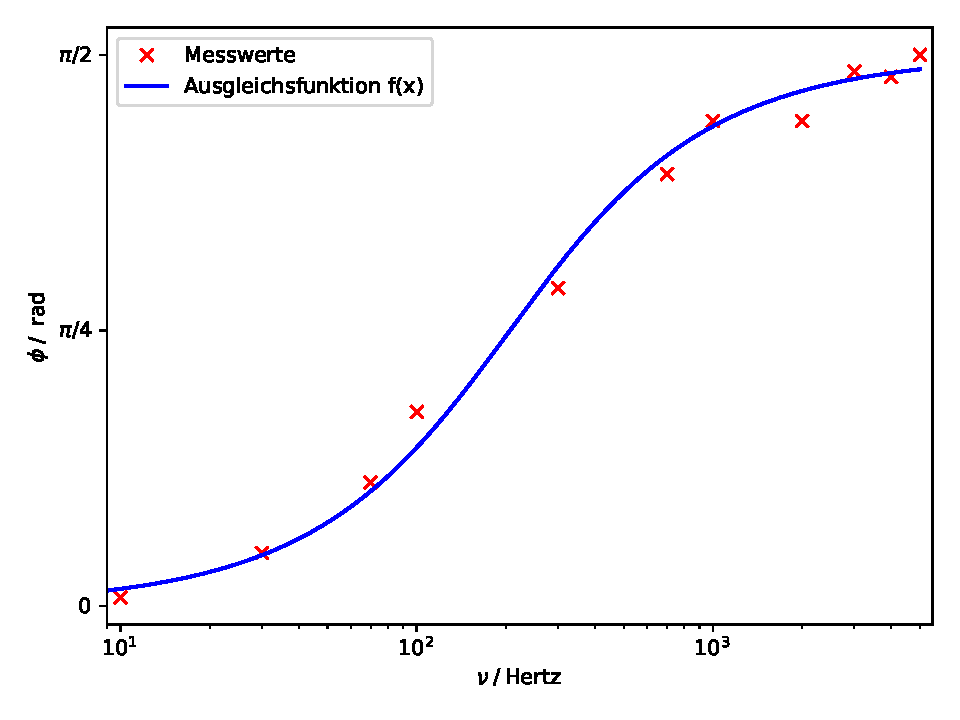
\includegraphics[height=9cm]{plot3.pdf}
  \caption{Lineare Ausgleichsrechnung zur Energiekalibration}
  \label{fig:plot3}
\end{figure}
Die Energiekalibration erfolgt somit gemäß
\begin{equation}
  \symup{E}_{\gamma} (x) = \SI{0.403169}{\kilo\electronvolt}\cdot x - \SI{3.034}{\kilo\electronvolt}
  \label{eqn:gerade}
\end{equation}
wobei x die Kanalnummer bezeichnet.
Der dazugehörige Fehler ergibt mittels Gleichung \ref{eqn:gaus} durch
\begin{equation}
   \increment \symup{E}_{\gamma} (x) =\sqrt{ (\SI{0.000029}{\kilo\electronvolt}\cdot x)^2 +
   (\SI{0.060}{\kilo\electronvolt})^2}
   \label{eqn:fgerade}
\end{equation}
\\
Zur Bestimmung der Vollenergienachweiswahrscheinlichkeit wird zunächst die Gleichung \ref{eqn:gausk}
integriert, um den Inhalt der Peaks zu bestimmen, wobei der Untegrund $a$ vorher abgezogen wird.
Es ergibt sich somit ein Linieninhalt von
\begin{equation}
  \symup{I} =\int_{-\infty}^{\infty} c \cdot \symup{e}^{(\frac{x-z}{b})^2} \symup{d}x
  = c \cdot b \cdot \sqrt{\pi}
  \label{eqn:inh}
\end{equation}
in Abhängigkeit der Parameter b und c.
Der Fehler ergibt sich durch Gleichung \ref{eqn:gaus} über die Gleichung
\begin{equation}
  \increment \symup{I} = \sqrt{ (\increment c \cdot b \cdot \sqrt{\pi})^{2}
   + (c \cdot \increment b \cdot \sqrt{\pi}})^{2} \: .
     \label{eqn:inhf}
\end{equation}
Mit den Werten aus Tabelle \ref{tab:tabe1} lassen sich somit die einzelnen Linieninhalte berrechen,
welche in Tabelle \ref{tab:tabe3} angegeben sind.
\begin{table}
  \centering
  \caption{Messwerte für den ersten Doppelspalt.}
   \begin{tabular}{S S| S S | S S}
    \toprule
    $x/\; \si{\mm}$& $A/\;\si{\nA}$ &
    $x/\; \si{\mm}$& $A/\;\si{\nA}$ &
    $x/\; \si{\mm}$& $A/\;\si{\nA}$ \\
    \midrule

    15.0& 4.6& 23.0& 25.0& 29.5& 6.0\\
    15.5& 4.2& 23.5& 30.0& 30.0& 5.3\\
    16.0& 4.0& 24.0& 35.0& 30.5& 4.9\\
    16.5& 4.0& 24.25& 36.0& 31.0& 4.7\\
    17.0& 4.4& 24.5& 37.0& 31.5& 4.4\\
    17.5& 5.5& 24.75& 38.0& 32.0& 4.2\\
    18.0& 6.6& 25.00& 37.0& 32.5& 3.8\\
    18.5& 7.7& 25.25& 36.0& 33.0& 3.6\\
    19.0& 8.2& 25.5& 36.0& 33.5& 3.2\\
    19.5& 8.4& 26.0& 33.0& 34.0& 3.2\\
    20.0& 8.4& 26.5& 28.5& 34.5& 3.2\\
    20.25& 8.4& 27.0& 23.0& 35.0& 3.3\\
    20.5& 8,7& 27.5& 18.0& 35.5& 3.4\\
    21.0& 9.8& 28.0& 13.5& 36.0& 3.5\\
    21.5& 12.0& 28.5& 10.0\\
    22.0& 15.0& 29.0& 7.8\\
    22.5& 20.0& 29.25& 6.7\\


   \bottomrule
  \end{tabular}
  \label{tab:tabelle3}
\end{table}

Zum Vergleich werden nun die Theoriewerte berrechnet, als Produkt
der Emissionswahrscheinlichkeiten P aus Tabelle \ref{tab:tabe2},
dem abgedeckten Raumwinkelanteil $\frac{\Omega}{4\pi}= 0.01558$, der errechneten Aktivität
$A =\SI{1599(29)}{\becquerel} $
und der Messzeit von $t = \SI{3598}{\second}$
\begin{equation}
  \symup{I}_{\text{theo}} = P\cdot \frac{\Omega}{4\pi} \cdot A \cdot t
  \label{eqn:itheo}
\end{equation}
mit dem Fehler über Gleichung \ref{eqn:gaus} von
\begin{equation}
  \increment \symup{I}_{\text{theo}} = \sqrt{ (\increment P\cdot \frac{\Omega}{4\pi} \cdot A \cdot t)^{2}
   + (P\cdot \frac{\Omega}{4\pi} \cdot \increment A \cdot t)^{2}} \: .
\end{equation}
Aus dem jeweiligen Quotienten
\begin{equation}
  \symup{Q} = \frac{\symup{I}}{\symup{I}_{\text{theo}}}
  \label{eqn:ven1}
\end{equation}
mit dem dazugehörigen Fehler
\begin{equation}
  \increment \symup{Q} = \sqrt{ (\frac{1}{\symup{I}_{\text{theo}} \cdot \increment \symup{I})^{2}
   + (\frac{\symup{I}}{\symup{I}_{\text{theo}}})^{2}}\cdot \increment \symup{I}_{\text{theo}})^{2}}
\end{equation}
ergibt sich somit jeweils die Nachweiswahrscheinlichkeit des Peaks, wie in Tabelle
\ref{tab:tabe4} dargestellt ist.
\begin{table}[H]
  \centering
   \begin{tabular}{c c c c}
    \toprule
    Nummer der Oberwelle & $ U_{\text Theorie,Rechteck}\: / \si{\volt} $ &
    $ U_{\text Theorie,Dreick}\: / \si{\volt} $ & $ U_{\text Theorie,Sägezahn}\: / \si{\volt} $ \\
    \midrule
    1 & 1145 & 182 & 573 \\
    2 & 0 & 0 & 286 \\
    3 & 573 & 20 & 191 \\
    4 & 0 & 0 & 143 \\
    5 & 229 & 7 & 115 \\
    6 & 0 & 0 & 96 \\
    7 & 164 & 4 & 82 \\
    8 & 0 & 0 & 72 \\
    9 & 127 & 2 & 64 \\
    10 & 0 & 0 & 57 \\
    \bottomrule
  \end{tabular}
  \caption{Eingestellte Schwingungsamplituden.}
  \label{tab:tabe4}
\end{table}

Da die Nachweiswahrscheinlichkeit im Allgemeinen energieabhängig ist, wird Q in
Abhängigkeit von $ \text{E}_{\gamma} $ dargestellt und mit einer Potenzfunktion der Form
\begin{equation}
  \symup{Q}(\text{E}_{\gamma}) = c\cdot (\text{E}_{\gamma}-a)^{d}
  \label{eqn:ven2}
\end{equation}
gefittet, wie in Abbildung \ref{fig:plot4} dargestellt ist.
Es ergeben sich hierbei die Parameter
\begin{align*}
  a &= -191 \pm 64 \\
  c &= 2474 \pm 3467 \\
  d &= -1.47 \pm 0.19 \: .
\end{align*}
 %Die Formel für die eigentliche Höhe eines
%gemessenen Peaks ergibt sich aus Gleichungen \ref{eqn:ven1} und \ref{eqn:ven2} durch Umstellen zu
%\begin{equation}
%  \symup{I}_{\text{theo}} = \frac{\symup{I}}{\symup{Q}}=\frac{\symup{I}}{c\cdot (\text{E}_{\gamma}-a)^{d}}
%  \label{eqn:ven}
%\end{equation}
%mit dem dazugehörigen Fehler
%\begin{equation}
%  \symup{I}_{\text{theo}} = \frac{\symup{I}}{\symup{Q}}=\frac{\symup{I}}{c\cdot (\text{E}_{\gamma}-a)^{d}}
%  NAMNAM
%  \label{eqn:ven}
%\end{equation}
\begin{figure}
  \centering
  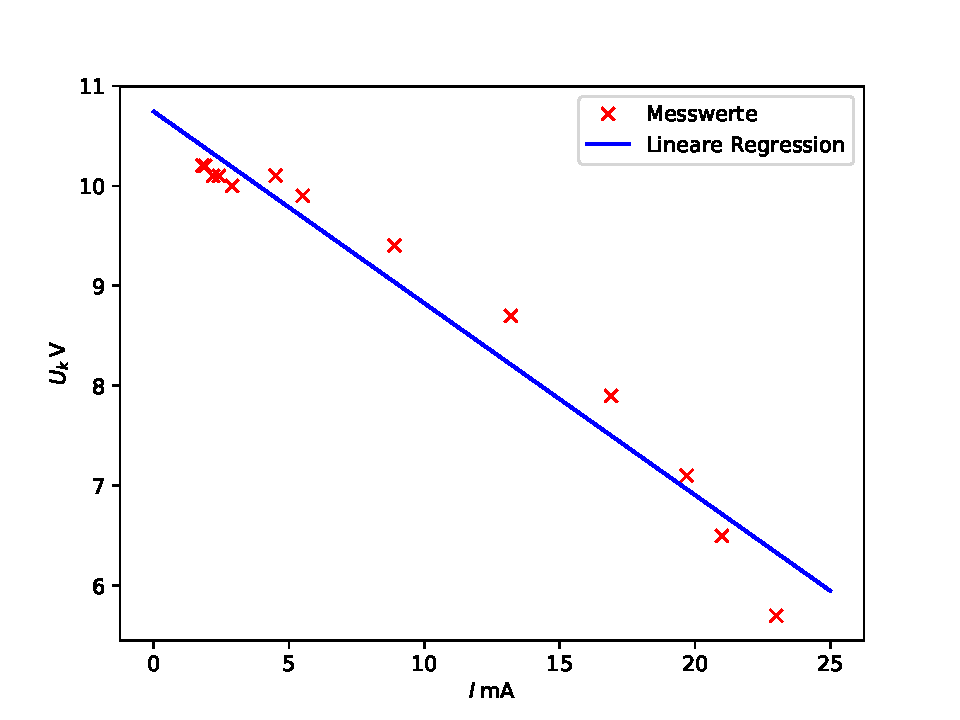
\includegraphics[height=9cm]{plot4.pdf}
  \caption{Werte zur Bestimmung der Vollenergienachweiswahrscheinlichkeit sowie gefittete Potenzfunktion}
  \label{fig:plot4}
\end{figure}

\subsection{Untersuchung eines monochromatischen Gamma-Spektrums}
Zur Untersuchung des monochromatischen Gamma-Spektrums wird das aufgenommene Spektrum
zunächst durch die Gleichung \ref{eqn:gerade} kalibriert, wobei sich der Fehler über
\ref{eqn:fgerade} ergibt. Die so erhaltenen Werte sind in Abbildung \ref{fig:plot5}
dargestellt, wobei auf Fehlerbalken aufgrund der geringen Fehler verzichtet wird. Die
Messzeit beträgt $\SI{2593}{\second}$ und es wurden 8191 Kanäle gemessen, wobei nur die
ersten 2000 dargestellt sind, da bei höheren Kanalnummern keine signifikanten Messwerte
mehr zu erkennen sind.
\begin{figure}
  \centering
  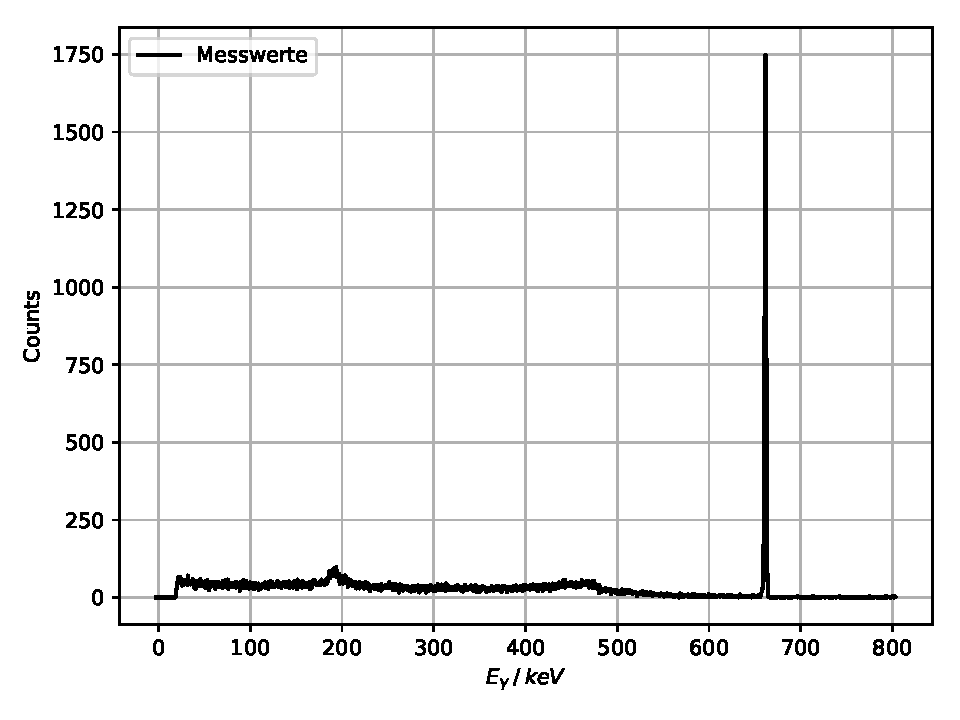
\includegraphics[height=9cm]{Cs.pdf}
  \caption{Kalibriertes Spektrum des $\ce{^{137}Cs}$-Strahlers }
  \label{fig:plot5}
\end{figure}
Zur Bestimmung der Energie wird die Vollenergielinie mit der Gaußverteilung aus Gleichung
\ref{eqn:gausk} gefittet, wobei sich die Parameter
\begin{align*}
  a &= 5.7 \pm 4.2 \\
  b &= 1674 \pm 17 \\
  c &= \SI{1.227(15)}{\kilo\electronvolt}\\
  z &= \SI{661.5985(98)}{\kilo\electronvolt} \:
\end{align*}
ergeben.
Die Energie des Strahlers ist dabei durch den Parameter $z$ gegeben, also
\begin{align*}
  \symup{E}_{Cs} = \SI{661.5985(98)}{\kilo\electronvolt} \: .
\end{align*}
Der Theoriewert von $\ce{^{137}Cs}$ beträgt $\SI{661.657(3)}{\kilo\electronvolt}$ \cite{lara}. \\
Der Bereich um die Vollenergielinie ist in
Abbildung \ref{fig:plot6} dargestellt, woraus sich die Halbwertsbreite und die
Zehntelwertsbreite ablesen lässt, wobei eine Ungenauigkeit durch
Ablesefehler von etwa $\SI{0.2}{\kilo\electronvolt}$ angenommen wird.
Es ergibt sich hierdurch
\begin{align*}
  \symup{E}_{1/2} = \SI{662.6(2)}{\kilo\electronvolt} -\SI{660.6(2)}{\kilo\electronvolt}
  =\SI{2.0(3)}{\kilo\electronvolt}\\
  \symup{E}_{1/10} = \SI{663.3(2)}{\kilo\electronvolt} -\SI{659.6(2)}{\kilo\electronvolt}
  =\SI{3.7(3)}{\kilo\electronvolt} \:
\end{align*}
woraus sich ein Verhältniss von
\begin{equation}
  \frac{\symup{E}_{1/2}}{\symup{E}_{1/10}} =  0.54 \pm 0.09 \:
\end{equation}
ergibt.
\begin{figure}
  \centering
  \includegraphics[height=9cm]{Plot6.pdf}
  \caption{Vollenergielinie}
  \label{fig:plot6}
\end{figure}
Die Halbwertsbreite einer Gaußkurve gemäß Gleichung \ref{eqn:gausk} ist durch die
Formel
\begin{equation}
  \symup{E}_{1/2} = 2c\cdot\sqrt{ln2}
\end{equation}
mit dem Fehler
\begin{equation}
  \increment \symup{E}_{1/2} = 2\increment b\cdot\sqrt{ln2} \: ,
\end{equation}
gegeben und beträgt somit
\begin{align*}
  \symup{E}_{1/2,theo} = \SI{1.701(21)}{\kilo\electronvolt} \: .
\end{align*}
Die Zehntelwertsbreite ergibt sich analog über die Gleichung
\begin{equation}
  \symup{E}_{1/10} = 2c\cdot\sqrt{ln10}
\end{equation}
mit dem Fehler
\begin{equation}
  \increment \symup{E}_{1/10} = 2\increment b\cdot\sqrt{ln10} \: ,
\end{equation}
zu
\begin{align*}
  \symup{E}_{1/10, theo} = \SI{5.651(69)}{\kilo\electronvolt} \: .
\end{align*}
Das Verhältniss dieser beiden Größen ist unabhängig von den jeweiligen Parametern der
Kurve stets
\begin{equation}
  \frac{\symup{E}_{1/2}}{\symup{E}_{1/10}} = \sqrt{\frac{ln2}{ln10}}
  \approx 0.549 \: ,
\end{equation}
Diese theoretisch erhaltenen Werte werden mit den abglesenen verglichen, wobei sich
die Abweichung über die Formel
\begin{equation}
  \frac{\lvert \text{Wert}_{\text{Theorie}}-\text{Wert}_{\text{Messung}}\rvert}{\text{Wert}_{\text{Theorie}}}
  \label{eqn:abw}
\end{equation}
berechnen lässt zu 1.64 \%. Diese Abweichung ist offensichtlich sehr gering und liegt innerhalb der
Ableseunsicherheit, was auf eine gute Beschreibung der Vollenergielinie
durch eine Gaußkurve schließen lässt. Die recht große Abweichung der Halb- und Zehntelwertsbreite
an sich lässt sich dadurch erklären, dass wohlmöglich eine falsche Maximalhöhe des Peaks angenommen
wurde.
Der Inhalt der Vollenergielinie ergibt sich durch Gleichungen \ref{eqn:inh}
und \ref{eqn:inhf} zu
\begin{align*}
  \symup{I}_{VEL} =  3641 \pm 58 \: .
\end{align*}
\\
Aus den Messwerten und Abbildung \ref{fig:plot5} lässt sich erkennen, dass die
Compton-Kante bei etwa $\SI{478(3)}{\kilo\electronvolt}$ liegt, da dort (Kanalnummer
1198) das Spektrum ein lokales
Maximum von 53 Counts animmt und anschließend abfällt, wobei die Ableseunsicherheit auf etwa
$\SI{3}{\kilo\electronvolt}$ geschätzt wird.
Aus Gleichung \ref{eqn:kante} ergibt sich der theoretische Wert zu $\SI{477.280(90)}{\kilo\electronvolt}$
und die Abweichung somit zu 0.15 \%.
Um den Inhalt des Comptonkontinuums zu bestimmen wird der Bereich zwischen $\SI{20}{\kilo\electronvolt}$
und $\SI{478}{\kilo\electronvolt}$ mit der Funktion aus Gleichung \ref{eqn:diffCompton} gefittet,
wobei der Term $a =\frac{3}{8}\sigma_{\text{Th}}\frac{1}{m_0 c^2 e^2}$ als Fitparameter
verwendet wird. Für diesen ergibt sich
\begin{align*}
  a =  4.297 \pm 0.056 \: .
\end{align*}
Dieser Wert wird nun verwendet, um die Funktion numerisch in dem Bereich zwischen $\SI{20}{\kilo\electronvolt}$
und $\SI{478}{\kilo\electronvolt}$
zu integrieren, wodurch sich der Inhalt des Comptonkontinuums zu
\begin{align*}
  \symup{I}_{Compton} =  16266 \pm 214
\end{align*}
ergibt.

Der Rückstreupeak wird erneut mit der Gleichung \ref{eqn:gausk} gefittet, wodurch sich
die Parameter
\begin{align*}
  a &= 65.8 \pm 2.0 \\
  b &= 36 \pm 28 \\
  c &= \SI{0.28(28)}{\kilo\electronvolt}\\
  z &= \SI{193.78(24)}{\kilo\electronvolt} \:
\end{align*}
ergeben, der Rückstreupeak liegt also bei $\SI{193.78(24)}{\kilo\electronvolt}$.
Der Theoriewert nach Gleichung \ref{eqn:Rückstreu} ergibt sich zu $\SI{184.3184(76)}{\kilo\electronvolt}$.
\\
Zur Bestimmung der Absorptionswahrscheinlichkeiten wird die Formel
\begin{equation}
  \symup{p} = 1-\exp{-\mu \cdot l}
\end{equation}
verwendet, wobei $l$ die Länge des Detektors, in diesem Fall also $\SI{3.9}{\centi\meter}$, bezeichnet
und $\mu$ den Extinkionskoeffizient, welcher für den Comptoneffekt etwa
$\mu_{c}=\SI{0.38}{\per\centi\meter}$ und für den Photoeffekt etwa
$\mu_{p}=\SI{0.008}{\per\centi\meter}$ beträgt.
Dies führt zu Absorptionswahrscheinlicheiten von
\begin{align*}
  \symup{p}_{c} = 0.7728 \\
  \symup{p}_{p} = 0.0307 \: ,
\end{align*}
sodass sich theoretisch ein Verhältniss zwischen den Inhalten des Photopeaks und des
Comptonkontinuums von
\begin{equation*}
  (\frac{\symup{I}_{VEL}}{\symup{I}_{Compton}})_{\text{theo}} = 1-\symup{e}{-\mu \cdot l}
  = 0.03975
\end{equation*}
ergeben sollte. Das tatsächliche Verhältniss aus den Messdaten beträgt
\begin{equation*}
  \frac{\symup{I}_{VEL}}{\symup{I}_{Compton}}
  = 0.224 \pm 0.005
\end{equation*}
und weist somit eine Abweichung von 463.52 \% auf, gemäß Formel \ref{eqn:abw}.


\subsection{Aktivitätsbestimmung}
Bei dem dritten vermessenen Spektrum soll zunächst festgestellt werden, ob es sich bei der gemessenen
Probe um einen $\ce{^{133}Ba}$-Strahler oder einen $\ce{^{125}Sb}$-Strahler handelt. Zu diesem
Zweck wird das Spektrum zunächst gemäß Gleichung \ref{eqn:gerade} kalibriert, wie in Abbildung
\ref{fig:plot7} dargestellt ist. Die Messzeit beträgt $\SI{4378}{\second}$; von den 8191 verwendeten
Kanälen werden nur die ersten 2000 verwendet, da darüber hinaus keine signifikanten
Messwerte mehr zu erkennen sind.
\begin{figure}
  \centering
  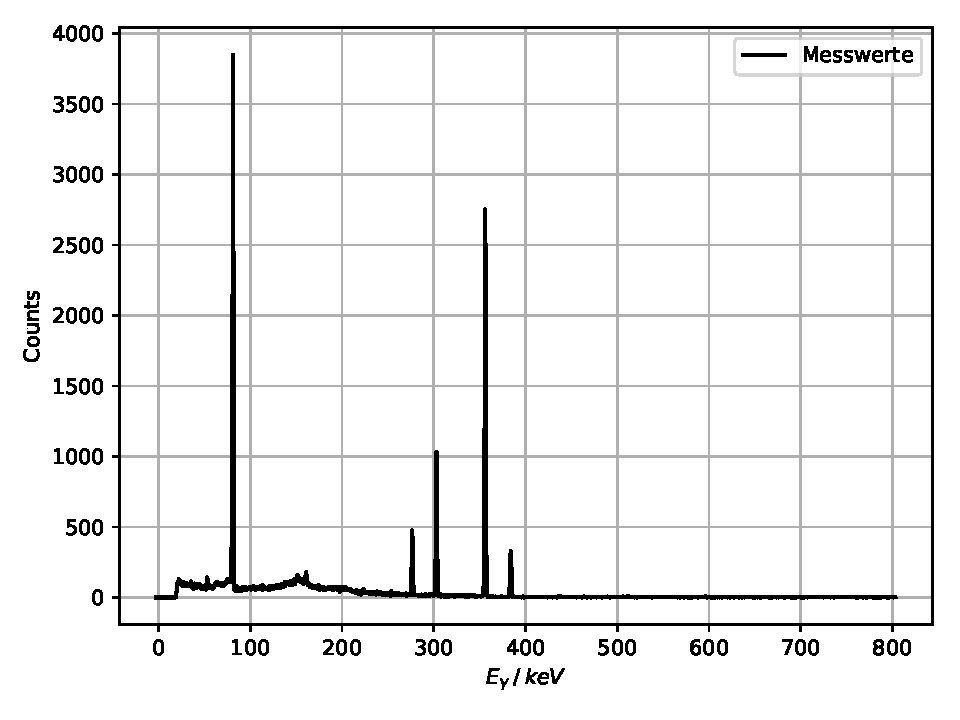
\includegraphics[height=9cm]{Ba.pdf}
  \caption{Unbekanntes Spektrum}
  \label{fig:plot7}
\end{figure}
Die Peaks werden erneut mit Gleichung \ref{eqn:gausk} gefittet und die resultierenden
Parameter in Tabelle \ref{tab:tabe5} dargestellt.
\begin{table}[H]
  \centering
  \caption{Bohrung 1 und 2, Vergleich der Sonden mit 1\;MHz und 2\;MHz.}
  \label{tab:tab5}
    \begin{tabular}{c c c c}
    \toprule
    Bohrung & $S_{\text{2\;MHz}}$/\;mm & $S_{\text{ 1\;MHz}}$/\;mm\\
    \midrule
    1 & 1,82 & 2,12\\
    2 & 1,83 & 1,97\\
    \bottomrule
    \end{tabular}
  \end{table}

Durch einen Vergleich mit der Datenbank
\cite{Lara} fällt auf, dass die Peaks mit denen von Barium übereinstimmen und es sich somit
bei der Probe offensichtlich um Barium handelt. Die Zuordnung zu den theoretischen Emissionslinien
und die entsprechenden Absorptionswahrscheinlickeiten sind in Tabelle \ref{tab:tabe6} angegeben.
\begin{table}[H]
  \centering
  \caption{Werte der Anpassungsschicht}
  \label{tab:tabe6}
    \begin{tabular}{S S S }
    \toprule
    $ \text{Zylinder} $ & $ \increment t [\mu\text{s}] $ &
    $ l_a \text{[mm]}$\\
    \midrule
    1 & 0.54 & 0.81 \\
    2 & 0.40 & 0.59 \\
    3 & 0.76 & 1.12 \\
    \text{1+2} & 0.49 & 0.73 \\
    4 & 0.70 & 1.03 \\
    \text{1+3} & 0.90 & 1.33 \\
    5 & 1.25 & 1.85 \\
    \text{1+4} & 0.69 & 1.02 \\
    6 & 0.44 & 0.66 \\

          \bottomrule
    \end{tabular}
  \end{table}

Zur Bestimmung der Aktivität wird mittels Gleichung \ref{eqn:inh} zunächst der Inhalt der Peaks errechnet.
Aus Gleichung \ref{eqn:itheo} lässt sich ein linearer Zusammenhang zwischen diesem Inhalt und der Aktivität
erkennen, wobei der Proportionalitätsfaktor durch
\begin{equation}
  l = P\cdot \frac{\Omega}{4\pi}\cdot t \cdot Q
  \label{eqn:lin}
\end{equation}
gegeben ist. Zur Bestimmung der Aktivität wird also eine Lineare Ausgleichsrechnung
gemäß Formel \ref{eqn:li} mit Wertepaaren aus $l$ und $\symup{I}$ durchgeführt,
wobei der Fitparameter a die Aktivität angibt. Dabei wird die $\SI{81.0657}{\kilo\electronvolt}$
außer Acht gelassen, da bei so niedrigen Energien der Quotient $Q$ der Vollenergienachweiswahrscheinlichkeit
zu ungenau ist. Somit ergeben sich die Parameter
\begin{align*}
  a = 416.4 \pm 2.7 \\
  b = 35 \pm 14
\end{align*}
und damit eine Aktivität von $\SI{416.4(27)}{\becquerel} $.
Die Wertepaare und die Ausgleichsgerade sind in Abbildung \ref{fig:plot9} dargestellt.
\begin{figure}
  \centering
  \includegraphics[height=9cm]{Plot9.pdf}
  \caption{Lineare Regression zur Aktivitätsbestimmung von $\ce{^{133}Ba}$}
  \label{fig:plot9}
\end{figure}



\subsection{Nuklididentikation}
Im letzten Versuchsteil wird eine Probe unbekannter Zusammensetzung untersucht, wobei die
Messzeit $\SI{4064}{\second}$ beträgt. Von den 8191 gemessenen Kanälen werden die ersten 6000 zur Auswertung
verwendet, die entsprechenden Messwerte werden gemäß Gleichung \ref{eqn:gerade} kalibriert und
sind in Abbildung \ref{fig:plot8} dargestellt.
\begin{figure}
  \centering
  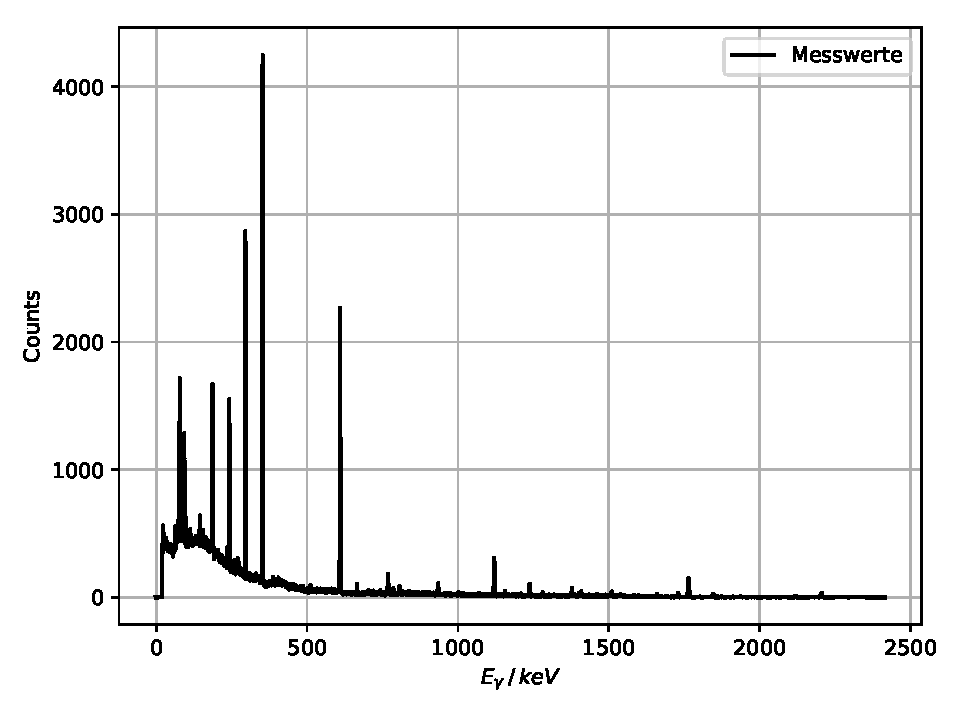
\includegraphics[height=9cm]{Un.pdf}
  \caption{Unbekanntes Spektrum}
  \label{fig:plot8}
\end{figure}

Um die Energie der Peaks zu bestimmen und sie somit zuordnen zu können, werden sie
wieder an die Gaußkurve gemäß Gleichung \ref{eqn:gausk} angepasst. Die Fitparameter sind in Tabelle
\ref{tab:tabe7} angegeben.

\begin{table}[H]
  \centering
  \caption{Parameter der gefitteten Gaußkurven}
  \label{tab:tabe7}
    \begin{tabular}{l l l l}
    \toprule
    $ a $ & $ b $ & $ c $
    & $ z \:/ \:\si{\kilo\electronvolt} $ \\
    \midrule
    593 \pm 23 & 1156 \pm 143 & 0.573 \pm 0.083 & 77.124 \pm 0.058 \\
    556 \pm 17 & 769 \pm 104 & 0.603 \pm 0.095 & 92.632 \pm 0.066 \\
    375.6 \pm 4.9 & 1335 \pm 25 & 0.772 \pm 0.017 & 186.090 \pm 0.012 \\
    252.8 \pm 6.2 & 1308 \pm 33 & 0.719 \pm 0.022 & 242.066 \pm 0.015 \\
    179.7 \pm 2.7 & 2711 \pm 14 & 0.7850 \pm 0.0048 & 295.3181 \pm 0.0033 \\
    130.2 \pm 4.2 & 4164 \pm 21 & 0.8586 \pm 0.0050 & 352.0054 \pm 0.0034 \\
    46.7 \pm 3.0 & 2230 \pm 12 & 1.1737 \pm 0.0076 & 609.2939 \pm 0.0052 \\
    31.3 \pm 1.1 & 64.9 \pm 4.2 & 1.33 \pm 0.10 & 665.409 \pm 0.070 \\
    31.3 \pm 1.3 & 158.5 \pm 4.6 & 1.451 \pm 0.051 & 768.246 \pm 0.034 \\
    30.9 \pm 1.0 & 38.9 \pm 3.9 & 1.29 \pm 0.16 & 785.87 \pm 0.10 \\
    30.7 \pm 1.0 & 46.6 \pm 4.1 & 1.20 \pm 0.13 & 806.244 \pm 0.085 \\
    26.3 \pm 1.1 & 72.9 \pm 3.7 & 1.68 \pm 0.10 & 934.015 \pm 0.067 \\
    18.2 \pm 1.9 & 292.3 \pm 5.8 & 1.782 \pm 0.043 & 1120.275 \pm 0.028 \\
    16.44 \pm 0.76 & 32.8 \pm 2.3 & 1.87 \pm 0.16  & 1155.44 \pm 0.10 \\
    13.1 \pm 1.1 & 98.2 \pm 3.1 & 2.037 \pm 0.078 & 1238.098 \pm 0.051 \\
    16.17 \pm 0.93 & 55.9 \pm 2.7 & 1.91 \pm 0.11 & 1377.862 \pm 0.074 \\
    17.5 \pm 1.3 & 25.6 \pm 3.8 & 1.95 \pm 0.36 & 1408.31 \pm 0.23 \\
    13.89 \pm 0.95 & 19.6 \pm 2.4 & 2.33 \pm 0.36 & 1509.44 \pm 0.22 \\
    4.78 \pm 0.63 & 12.2 \pm 1.3 & 2.96 \pm 0.40 & 1661.07 \pm 0.24 \\
    3.029 \pm 0.73 & 28.2 \pm 1.6 & 2.75 \pm 0.20 & 1729.76 \pm 0.12 \\
    3.0 \pm 1.79 & 145.9 \pm 3.9 & 2.725 \pm 0.093 & 1764.689 \pm 0.057 \\
    3.56 \pm 0.78 & 20.2 \pm 1.7 & 2.77 \pm 0.29 & 1847.40 \pm 0.18 \\
    0.71 \pm 0.87 & 29.1 \pm 1.6 & 3.35 \pm 0.24 & 2204.71 \pm 0.13 \\



          \bottomrule

    \end{tabular}
\end{table}

Die Linienenergien werden dann mit der Datenbank \cite{lara} abgeglichen und
passenden Nukliden zugeordent.
Diese Zuordnung ist in Tabelle \ref{tab:tabe8} zusammen mit den jeweiligen Emissionswahrscheinlichkeiten
dargestellt.
\begin{table}[H]
  \centering
  \caption{Werte der Messreihe die Wien-Robinson-brücke}
  \label{tab:tabe8}
    \begin{tabular}{c c c c}
    \toprule
    $ \nu \: / \: \si{\hertz} $ & $\text{U}_b \: / \: \si{\volt} $ &
    $\text{U}_s \: / \: \si{\volt} $ &
    $\frac{U_b}{U_s}$ \\
    \midrule
    20 & 0.120 & 3.08 & 0.039 \\
    50 & 0.248 & 4.56 & 0.054 \\
    100 & 0.320 & 4.64 & 0.069 \\
    150 & 0.264 & 4.56 & 0.058 \\
    200 & 0.136 & 4.50 & 0.030 \\
    220 & 0.072 & 4.48 & 0.016 \\
    230 & 0.032 & 4.48 & 0.007 \\
    240 & 0.024 & 4.48 & 0.005 \\
    242 & 0.016 & 4.48 & 0.004 \\
    250 & 0.040 & 4.48 & 0.009 \\
    265 & 0.080 & 4.48 & 0.018 \\
    300 & 0.298 & 4.56 & 0.065 \\
    500 & 0.704 & 4.56 & 0.154 \\
    1000 & 1.17 & 4.32 & 0.271 \\
    3000 & 1.41 & 4.28 & 0.330 \\
    10000 & 1.44 & 4.24 & 0.340 \\
    20000 & 1.44 & 4.24 & 0.340 \\
    30000 & 1.44 & 4.24 & 0.340 \\

    \bottomrule
    \end{tabular}
\end{table}

Alle identifizierten Nuklide gehören zu der Uran-Radium Zerfallsreihe, welche auch als 4n+2
Reihe bekannt ist. Es lässt sich also vermuten, dass die Probe ursprünglich zum Teil aus
$\ce{^{238}U}$ oder $\ce{^{234}Th}$ bestand, welches über  die Zeit zerfallen ist und somit die
radioaktiven Tochternuklide $\ce{^{226}Ra}$, $\ce{^{214}Pb}$ und $\ce{^{214}Bi}$ erklärt.
Alle weiteren Nuklide der Reihe haben keine, oder zumindest nur sehr schwache
Gammasignaturen, sodass diese nicht detektiert werden können.
Für die Aktivitätsbestimmung sind nur bei $\ce{^{214}Pb}$ und $\ce{^{214}Bi}$ genügend
Linien vorhanden um eine nicht allzu ungenaue Rechnung durchführen zu können. Das Vorgehen ist analog zur
Bestimmung der Aktivität von $\ce{^{133}Ba}$ und die resultierenden Ausgleichsgeraden sind in den
Abbildungen \ref{fig:plot11} und \ref{fig:plot12} dargestellt. Bei der Aktivitätsbestimmung
von $\ce{^{214}Pb}$ wurde die $\SI{77.1088}{\kilo\electronvolt}$ Linie außer acht gelassen,
da hier der Quotient $Q$ zu ungenau ist.
Es ergeben sich die Fitparameter
\begin{align*}
  a_{\text{Pb}} &= 1106 \pm 17 \\
  b_{\text{Pb}} &= -6\pm 69 \\
  a_{\text{Bi}} &= 1442 \pm 89 \\
  b_{\text{Bi}} &= 7 \pm 21 \\
\end{align*}
und somit Aktivitäten von $\SI{1106(17)}{\becquerel} $ für $\ce{^{214}Pb}$ und
$\SI{1442(89)}{\becquerel} $ für $\ce{^{214}Bi}$.
\begin{figure}
  \centering
  \includegraphics[height=9cm]{Plot11.pdf}
  \caption{Lineare Regression zur Aktivitätsbestimmung von $\ce{^{214}Pb}$}
  \label{fig:plot11}
\end{figure}
\begin{figure}
  \centering
  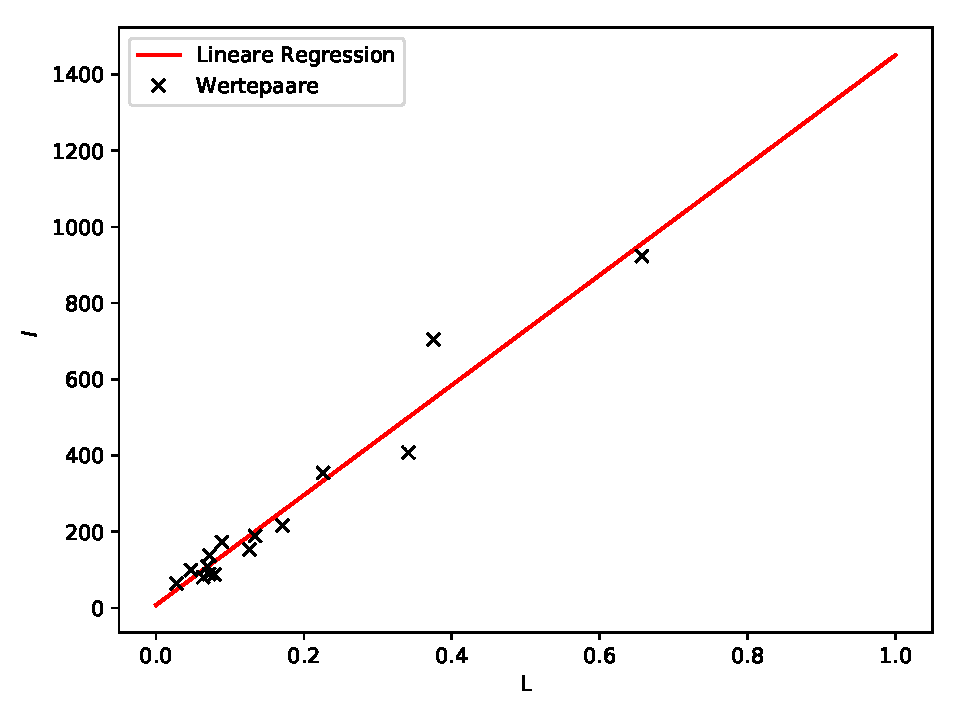
\includegraphics[height=9cm]{plot12.pdf}
  \caption{Lineare Regression zur Aktivitätsbestimmung von $\ce{^{214}Bi}$}
  \label{fig:plot12}
\end{figure}

\section{Diskussion}
Die lineare Regression zur Bestimmung der Energiekalibration liefert sehr geringe Ungenauigkeiten
der Fitparameter und scheint somit sehr exakt zu sein, was für ein gutes Auflösungsvermögen
des Detektors spricht. Die Parameter des Fits für die Vollenergienachweiswahrscheinlichkeit sind hingegen
mit einem großen relativen Fehler behaftet, welche teilweise sogar größer als der
eigentliche Wert sind. Dies lässt darauf schließen, dass eine Potenzfunktion
nicht vollständig zur Beschreibung der Energieabhängigkeit geeignet ist und
eine andere Funktion eventuell besser zu den Daten passen würde. \\
Die Abweichung in der gemessenen Energie des $\ce{^{137}Cs}$-Strahlers beträgt lediglich
0.0088\%, wodurch erneut die gute Energieauflösung gezeigt wird. Wie bereits erwähnt
ist die Beschreibung der Peaks durch Gaußkurve sehr genau und weißt im Verhältniss
von Halb- und Zehntelwertsbreite nur eine Abweichung von 1.64 \% auf. \\
Auch die Componkante und das Comptonkontinuum können recht genau bestimmt werden,
jedoch ergibt sich bei dem Rückstreupeak eine Abweichung von 5,14 \% , wobei der Theoriewert etwa 39,44
Fehlerintervalle von dem experimentellen Wert abweicht. Es wird somit vermutlich ein systematischer Fehler
vorliegen. \\
Auch bei dem Verhältniss des Inhalts von Comptonkontinuum und Photopeak gibt es eine
sehr große Abweichung, was vermutlich daran liegt, dass Mehrfachstreuung beim
Comptoneffekt in den theoretischen Formeln nicht berücksichtigt wird. Durch diese
Mehrfachstreuung deponiert die Gammastrahlung einen größeren Anteil oder eventuell auch die
gesamte Energie in dem Detektor, sodass der Inhalt des Comptonkontinuums sinkt und der
Inhalt des Photopeaks steigt, was den Betrag des Verhältnisses ansteigen lässt. \\
Die Aktivität lässt sich ebenfalls bis auf einen geringen
relativen Fehler bestimmen und auch die Zuordnung der Proben ist aufgrund der
guten Energieauflösung problemlos möglich. Lediglich die $\SI{92.38(1)}{\kilo\electronvolt}$-Linie
und die $\SI{92.80(1)}{\kilo\electronvolt}$-Linie von $\ce{^{234}Th}$ können nicht
getrennt aufgelöst werden, sondern erscheinen als ein einzelner Peak. Hier liegt offensichtlich
die Grenze des Auflösungsvermögens.


\printbibliography{}

\end{document}
=======
\documentclass[
  bibliography=totoc,     % Literatur im Inhaltsverzeichnis
  captions=tableheading,  % Tabellenüberschriften
  titlepage=firstiscover, % Titelseite ist Deckblatt
]{scrartcl}

% Paket float verbessern
\usepackage{scrhack}

% Warnung, falls nochmal kompiliert werden muss
\usepackage[aux]{rerunfilecheck}

% unverzichtbare Mathe-Befehle
\usepackage{amsmath}
% viele Mathe-Symbole
\usepackage{amssymb}
% Erweiterungen für amsmath
\usepackage{mathtools}

% Fonteinstellungen
\usepackage{fontspec}
% Latin Modern Fonts werden automatisch geladen
% Alternativ zum Beispiel:
%\setromanfont{Libertinus Serif}
%\setsansfont{Libertinus Sans}
%\setmonofont{Libertinus Mono}

% Wenn man andere Schriftarten gesetzt hat,
% sollte man das Seiten-Layout neu berechnen lassen
\recalctypearea{}

% deutsche Spracheinstellungen
\usepackage{polyglossia}
\setmainlanguage{german}


\usepackage[
  math-style=ISO,    % ┐
  bold-style=ISO,    % │
  sans-style=italic, % │ ISO-Standard folgen
  nabla=upright,     % │
  partial=upright,   % ┘
  warnings-off={           % ┐
    mathtools-colon,       % │ unnötige Warnungen ausschalten
    mathtools-overbracket, % │
  },                       % ┘
]{unicode-math}

% traditionelle Fonts für Mathematik
\setmathfont{Latin Modern Math}
% Alternativ zum Beispiel:
%\setmathfont{Libertinus Math}

\setmathfont{XITS Math}[range={scr, bfscr}]
\setmathfont{XITS Math}[range={cal, bfcal}, StylisticSet=1]

% Zahlen und Einheiten
\usepackage[
  locale=DE,                   % deutsche Einstellungen
  separate-uncertainty=true,   % immer Fehler mit \pm
  per-mode=symbol-or-fraction, % / in inline math, fraction in display math
]{siunitx}

% chemische Formeln
\usepackage[
  version=4,
  math-greek=default, % ┐ mit unicode-math zusammenarbeiten
  text-greek=default, % ┘
]{mhchem}

% richtige Anführungszeichen
\usepackage[autostyle]{csquotes}

% schöne Brüche im Text
\usepackage{xfrac}

% Standardplatzierung für Floats einstellen
\usepackage{float}
\floatplacement{figure}{htbp}
\floatplacement{table}{htbp}

% Floats innerhalb einer Section halten
\usepackage[
  section, % Floats innerhalb der Section halten
  below,   % unterhalb der Section aber auf der selben Seite ist ok
]{placeins}

% Seite drehen für breite Tabellen: landscape Umgebung
\usepackage{pdflscape}

% Captions schöner machen.
\usepackage[
  labelfont=bf,        % Tabelle x: Abbildung y: ist jetzt fett
  font=small,          % Schrift etwas kleiner als Dokument
  width=0.9\textwidth, % maximale Breite einer Caption schmaler
]{caption}
% subfigure, subtable, subref
\usepackage{subcaption}

% Grafiken können eingebunden werden
\usepackage{graphicx}
% größere Variation von Dateinamen möglich
\usepackage{grffile}

% schöne Tabellen
\usepackage{booktabs}

% Verbesserungen am Schriftbild
\usepackage{microtype}

% Literaturverzeichnis
\usepackage[
  backend=biber,
]{biblatex}
% Quellendatenbank
\addbibresource{lit.bib}
\addbibresource{programme.bib}

% Hyperlinks im Dokument
\usepackage[
  unicode,        % Unicode in PDF-Attributen erlauben
  pdfusetitle,    % Titel, Autoren und Datum als PDF-Attribute
  pdfcreator={},  % ┐ PDF-Attribute säubern
  pdfproducer={}, % ┘
]{hyperref}
% erweiterte Bookmarks im PDF
\usepackage{bookmark}

% Trennung von Wörtern mit Strichen
\usepackage[shortcuts]{extdash}

\author{%
  AUTOR A\\%
  \href{mailto:authorA@udo.edu}{authorA@udo.edu}%
  \texorpdfstring{\and}{,}%
  AUTOR B\\%
  \href{mailto:authorB@udo.edu}{authorB@udo.edu}%
}
\publishers{TU Dortmund – Fakultät Physik}


\subject{Versuch 401}
\title{Das Michelson-Interferometer}
\date{%
  Durchführung: 10.04.2018
  \hspace{3em}
  Abgabe: 17.04.2018
}

\begin{document}

\maketitle
\thispagestyle{empty}
\tableofcontents
\newpage

\section{Zielsetzung}
Ziel ist es für eine unbekannte Probe die aktiven Isotope und deren Aktivität zu ermitteln,
dafür ist es zuvor notwendig mit bekannten Elementen die Detektoreigenschaften
zu bestimmen.

\section{Theorie}
\subsection{Wechselwirkung von Strahlung mit Materie}
Wechselwirkt Strahlung mit Materie, so wird die Intensität der Strahlung durch das Material
abgeschwächt, diese Intensitätsabnahme kann allgemein über das Lambert-Beersche-Gesetz beschrieben werden:
\begin{equation}
  I(x)=I_0\cdot\exp(-\mu x).
  \label{eqn:lambert}
\end{equation}
Dabei bezeichnet $\mu$ den Extinktionskoeffizienten oder auch Abschwächungskoeffizient genannt, dieser
setzt sich aus Absorption und Streuung zusammen und lässt sich durch die Formel
\begin{equation}
  \mu=Zn\sigma
\end{equation}
beschreiben. Z bezeichnet die Ordnungszahl des Materials, n die Teilchenzahldichte und $\sigma$ den
Wirkungsquerschnitt der sich aus den verschiedenen Wechselwirkungen zusammensetzt.
\begin{figure}[H]
  \centering
  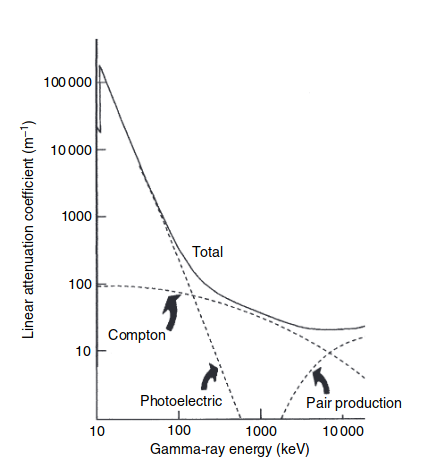
\includegraphics[height=8cm]{Extin.png}
  \caption{Der Extinkionskoeffizient in Abhängigkeit der Energie für verschiedene Prozesse. \cite{Gilmore2}}
  \label{fig:Extin}
\end{figure}

Wie in Abbildung \ref{fig:Extin} zu sehen ist, dominieren bei verschiedenen Energien
unterschiedliche Prozesse. Für geringe Energien dominiert der Photoeffekt, welcher mit
steigender Energie abnimmt, dadurch gewinnt der Comptoneffekt an Bedeutung. Für hohe
Energien dominiert die Paarerzeugung.
Da diese drei Prozesse für die Wechselwirkung von Gammaquanten mit Materie von großer Bedeutung sind
werden sie im Folgenden näher betrachtet.
\cite{Springer3}
\\
\\
\textbf{1. Photoeffekt}\\
Ein Gammaquant wird von einem kernnahen Hüllenelektron (bevorzugt aus der K-Schale) absorbiert,
wodurch das Hüllenelektron ausgelöst wird. Voraussetzung für diesen Effekt ist, dass das Gammaquant
mindestens die Bindungsenergie des Elektrons besitzt, überschüssige Energie wird als kinetische
Energie an das Elektron übertragen.
Das so entstandene "Loch" in der Elektronenhülle wird durch ein energiereicheres Hüllenelektron
gefüllt welches bei dem Übergang aus einer höheren Schale in eine niedrigere Schale
charakteristische Röntgenstrahlung emittiert.
Da sowohl die Röntgenstrahlung als auch das ausgelöste Elektron im Detektor verbleiben und
dort detektiert werden, verbleibt beim Photoeffekt die gesamte Gammaenergie im Detektor, weshalb
der Photopeak besonders wichtig für die Gammaspektroskopie ist.
Der differentielle Wirkungsquerschnitt der Energie lässt sich über die Formel
\begin{equation}
  \frac{d \sigma}{d E} = \bigg(-\frac{64}{7E^{9}}\bigg)^{1/2}\alpha^4 Z^5\sigma_{Th}
  \label{eqn:diffPhoto}
\end{equation}
beschreiben, wobei $\sigma_{Th}$ den Thomson-Wirkungsquerschnitt $\sigma_{Th} = \frac{8}{3}\pi r_{e}^2$
beschreibt mit $r_e$ als klassischen Elektronenradius.
(Thomson-Streuung: Streuung niederenergetischer Photonen an Elektronen) \cite{Springer3}
Der totale Wirkungsquerschnitt für den Photoeffekt ist von der Ordnungszahl des Materials
und der Photonenergie abhängig:
\begin{equation}
  \sigma_{\text{Photo}}\sim Z^5\cdot E_{\gamma}^{-7/2}.
  \label{eqn:WQphoto}
\end{equation}
\cite{Karlsruhe}
\\
\\

\textbf{2. Comptoneffekt}\\
Der Comptoneffekt beschreibt die Streuung von Photonen an äußeren Hüllenelektronen. Da
diese Streuung sehr stark winkelabhängig ist, kann von der gemessenen Elektronenenergie
nicht auf die Energie des Gammaquants geschlossen werden wodurch sich ein kontinuierliches
Spektrum, das Comptonkontinuum bildet. Dieses Spektrum bricht an der Comptonkante ab, hier
beträgt der Streuwinkel 180° und der Energieübertrag $E_{\text{max}}$ ist maximal, trotzdem gibt das
Gammaquant nicht seine gesamte Energie ab
\begin{equation}
  E_{max}=E_{\gamma}\cdot\frac{2\epsilon}{1+2\epsilon}\;\;<E_{\gamma}.
  \label{eqn:kante}
\end{equation}
\cite[Springer3]
Hier ist der Wirkungsquerschnitt über die Klein-Nishina-Formel gegeben, aus dieser ergibt sich der
differentielle Wirkungsquerschnitt:
\begin{equation}
  \frac{d\sigma}{dE}=\frac{3}{8}\sigma_{\text{Th}}\frac{1}{m_0 c^2 e^2}\bigg(2+\bigg(\frac{E}{h\nu-E} \bigg)^2 \bigg[\frac{1}{\epsilon^2}+
  \frac{h\nu-E}{h\nu}-\frac{2}{\epsilon}\bigg(\frac{h\nu-E}{h\nu}\bigg) \bigg]\bigg)
  \label{eqn:diffCompton}
\end{equation}
mit $\epsilon=\sfrac{E_{\gamma}}{m_e c^2}$.
Für den totalen Wirkungsquerschnitt gilt der Zusammenhang
\begin{equation}
  \sigma_{\text{Compton}}\sim \frac{Z}{E_{\gamma}}.
  \label{eqn:WPCompton}
\end{equation}
\\
\\
\textbf{3. Paarerzeugung}\\
Sind die Photonen energiereich genug können Elektron-Positron-Paare erzeugt werden, dafür müssen
die Photonen eine Mindestenergie von $E=2 m_0 c^2$ besitzen, also die doppelte
Ruheenergie des Elektrons.
Das so entstandene Positron annihiliert mit den im Detektor vorhandenen Elektronen und es
entstehen zwei Photonen. Wenn beide Photonen den Detektor verlassen wird dies als double-escape
bezeichnet, verlässt nur eins den Detektor entsteht der single-escape Peak.
Der differentielle Wirkungsquerschnitt für den Prozess der Paarerzeugung ist durch
\begin{equation}
  \frac{d\sigma}{dE}= \frac{28\alpha Z^2 r_{e}^2}{9E_{\gamma}}
  \label{eqn:diffPaar}
\end{equation}
gegeben, während der totale Wirkungsquerschnitt folgende Proportionalität besitzt:
\begin{equation}
  \sigma_{\text{Paar}}\sim Z^2\cdot\ln\Bigg(\frac{2E_{\gamma}}{m_e c^2}\Bigg).
  \label{eqn:WQPaar}
\end{equation}
\\

Eine Übersicht über die möglichen Wechselwirkungen von Gammaquanten mit Materie liefert
Abbildung \ref{fig:Effekt}.
\begin{figure}[H]
  \centering
  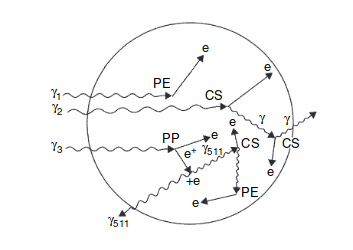
\includegraphics[height=5cm]{Effekte.png}
  \caption{Übersicht der Prozesse im Detektor. \cite{Gilmore2}}
  \label{fig:Effekt}
\end{figure}


\subsection{Grundlagen der Halbleiterinstrumente}
Halbleiter werden zwischen direkten und indirekten Halbleitern unterschieden, dies wird
in Abbildung \ref{fig:Band} dargestellt. Bei direkten Halbleitern
liegt das Maximum des Valenzbands genau unter dem Minimum des Leitungsbandes, somit ist ein direkter Bandübergang möglich.
Bei indirekten Halbleitern liegen Minima und Maxima nicht übereinander, für diesen indirekten Bandübergang ist
ein weiteres Photon nötig.\\

\begin{figure}
  \centering
  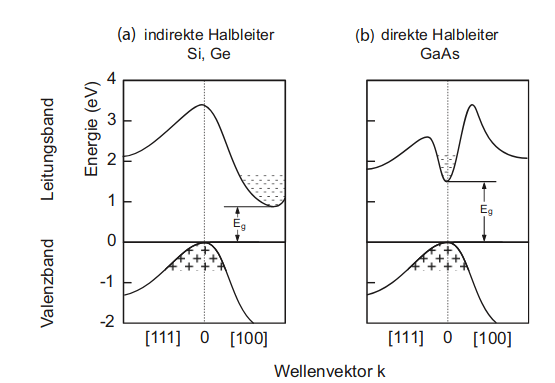
\includegraphics[height=6cm]{Band.png}
  \caption{Bandstruktur für direkte und indirekte Halbleiter.}
  \label{fig:Band}
  \cite{Springer3}
\end{figure}

Außerdem werden die Eigenschaften von Halbleitern durch ihre Dotierung beeinflusst. Germanium besitzt
beispielsweise 4 Valenzelektronen, wird nun ein Material mit fünf Valenzelektronen hinzugegeben bleibt nach
Eingehen der Bindungen ein freies Elektron übrig, somit dominieren die Elektronen als Ladungsträger und es handelt
sich um einen n-dotierten Halbleiter.
Wird stattdessen ein dreiwertiges Element verwendet bleibt ein Loch, somit stehen die Löcher als
positive Ladungsträger zur Verfügung und es handelt sich um einen p-dotierten Halbleiter.\\

\begin{figure}[H]
  \centering
  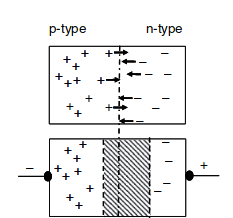
\includegraphics[height=6cm]{pn.png}
  \caption{Bildung einer Verarmungsschicht im pn-Übergang und Verbreiterung dieser durch
  anlegen einer äußeren Spannung.}
  \label{fig:pn}
  \cite{Gilmore2}
\end{figure}

Wie in Abbildung \ref{fig:pn} gezeigt entsteht ein pn-Übergang wenn p- und n-dotierte Halbleiter zusammengebracht werden,
Elektronen und Löcher vernichten sich in einem Teilbereich wodurch eine Verarmungszone entsteht.
Durch anlegen einer äußeren Spannung kann die Größe der Verarmungszone verändert werden. Für die
Verwendung als Detektor ist eine große Verarmungszone gewünscht, da dieser Bereich den
Detektorbereich bildet, also wird die Spannung in Sperrrichtung angelegt.


\subsection{Der Halbleiterdetektor}
Bei dem verwendeten Detektor handelt es sich um einen koaxialen Ge-Detektor wie in Abbildung
\ref{fig:Aufbau} zu sehen ist. Der gesamte Detektor befindet sich unter einer Aluminium
Schutzhaube und ist von außen mit Li-Atomen n-dotiert, wodurch die Oberfläche
gut leitend wird. Im Inneren befindet sich eine Bohrung, diese innere Oberfläche ist
mit Au-Atomen p-dotiert. (Die Dotierung ist hier etwas anders als oben beschrieben, da es sich um
Metall-Halbleiterkontakte handelt.) An diese dotierten Schichten wird die
äußere Spannung angelegt, die n-dotierte Schicht dient als Anschluss für den Pluspol.
Durch die p- und n-dotierten Bereiche bildet sich eine
Verarmungszone im Detektor die den Detektorbereich bildet. Somit müssen die Gammaquanten erst
die Al-Schicht und die Li-Schicht durchdringen um detektiert zu werden, dadurch kommt es zu einer
unteren Nachweisenergie der Gammaenergie, diese liegt bei 40 bis 50\;keV.
Dieser Gesamte Aufbau, wie in Abbildung \ref{fig:Aufbau} gezeigt befindet sich in einem
Bleigehäuse welches von innen mit Kupferplatten ausgelegt ist. Das Bleigehäuse dient zur Abschiermung
äußerer Strahlung, während die Kupferplatten die aus dem Blei austretende Strahlung
abhalten sollen.

\begin{figure}
  \centering
  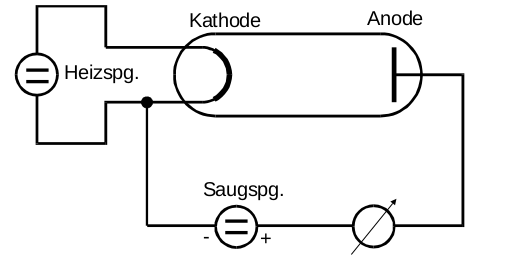
\includegraphics[height=7cm]{Aufbau.png}
  \caption{Schematischer Aufbau des Ge-Detektors. \cite{skript}}
  \label{fig:Aufbau}
\end{figure}

Dringt ein Gammaquant in die Verarmungszone ein wechselwirkt es mit der Materie und kann
z.B. ein Elektron auslösen welches mit anderen Elektronen stößt und ein Elektronen-Loch-Paar erzeugt.
Durch die angelegte Spannung wird das Paar räumlich getrennt wodurch eine Rekombination verhindert wird,
der dadurch entstehende Ladungsimpuls
wird verstärkt und bildet das Detektorsignal. Dieses ist proportional zu der einfallenden Photonenergie, da mit
einer höheren Energie auch mehr Elektronen-Loch-Paare erzeugt werden können.
Dringt das Gammaquant außerhalb der Verarmungszone in den Detektor ein rekombinieren die
Elektronen-Loch-Paare sofort, somit kann kein Signal gemessen werden.\\
Um Störsignale zu minimieren wird der Detektor mit Stickstoff auf 77\;K gekühlt, denn durch die
hohe externe Spannung kommt es zu thermischen Effekten wodurch sich noch Ladungsträger in der Verarmungszone
befinden und das Signal stören können.
\\
\\
\textbf{Eigenschaften eines Halbleiterdetektors}\\
Eine charakteristische Größe des Detektors ist das Auflösungsvermögen, dieses wird durch die
Halbwertsbreite $\Delta E_{1/2}$ der Impulshöhenverteilung beschrieben. Energien mit den Mittelwerten
$E_1$ und $E_2$ können noch voneinander unterschieden werden, wenn der Energieunterschied mindestens
$\Delta E_{1/2}$ beträgt.

Die Vollenergienachweiswahrscheinlichkeit eines Detektors gibt die Nachweiswahrscheinlichkeit eines Detektors
in Abhängigkeit der Energie an. Um sie zu bestimmen wird aus der aktuellen Aktivität der Probe der
theoretische Linieninhalt bestimmt, der Quotient aus gemessenem Linieninhalt und theoretischem
Linieninhalt gibt die Nachweiswahrscheinlichkeit des Detektors an.

\subsection{Das Spektrum eines monochromatischen Gammastrahlers}
Das Spektrum eines monochromatischen Gammastrahlers zeigt mehrere Besonderheiten auf, wie in Abbildung \ref{fig:Spektrum} zu
sehen. Wesentliche Bestandteile sind das Comptonkontinuum mit der Comptonkante, der Rückstreupeak
und der Photopeak. Der Photopeak entsteht dadurch, dass die Gammaquanten ihre gesamte Energie im Detektor deponieren
und wird daher auch Vollenergiepeak genannt. Er entsteht wenn die Gammaquanten im Detektor durch
Comptonstreuung genügend Energie verlieren bis der Photoeffekt eintreten kann und die restliche Energie
an den Detektor abgegeben wird. Auf diese Weise deponieren die Gammaquanten ihre gesamte Energie im
Detektor, so dass das Maximum des Photopeaks die Energie der Gammastrahlung angibt.\\
Das Comptonkontinuum entsteht durch Comptonstreuung der Gammaquanten, erfolgt die Streuung im
180° Winkel wobei der Energieübertrag maximal ist entsteht die Comptonkante. Da durch mehrfache
Comptonstreuung ein größerer Energieübertrag möglich ist als duch eine einmalige Streuung im 180° Winkel ist die
Componkante ausgeschmiert.\\
Da die Strahlung der Probe keine Vorzugsrichtung hat, wechselwirken einige Gammaquanten auch mit der
Abschirmung des Detektors und verlieren so Energie, werden sie dann so zurückgestreut, dass sie den
Detektor erreichen bilden sie den Rückstreupeak, dieser liegt bei
\begin{equation}
  E_{\text{Rück}}=E_{\gamma}\frac{1}{1+2\epsilon}
  \label{eqn:Rückstreu}
\end{equation}
Zwei weitere mögliche Peaks sind double- und single-escape Peak. Fällt ein Gammaquant in den Detektor und wechselwirkt über
Paarerzeugung entsteht ein Elektron und ein Positron, das Positron annihiliert mit den Elektronen der umgebenden Materie wobei
zwei Photonen erzeugt werden. Verlässt eins dieser Photonen den Detektor komm es zu single-escape Peak, verlassen beide
Photonen den Detektor entsteht der double-escape Peak.
\cite{Gilmore2}


\begin{figure}
  \centering
  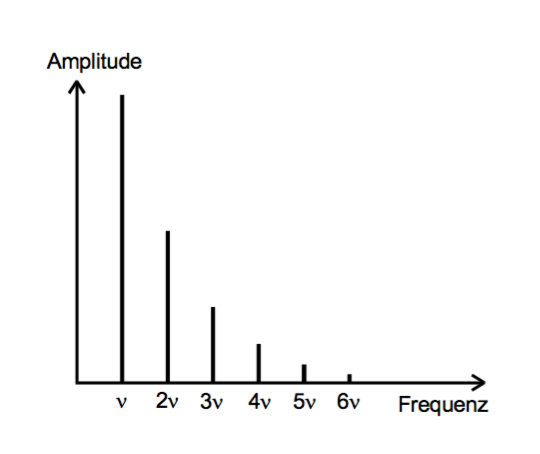
\includegraphics[height=7cm]{Spektrum.png}
  \caption{Gammaspektrum von $\ce{^{28}Al}$. Die Componkante ist hier nicht eingezeichnet, sie ist der Peak zwischen single escape und Photopeak,
  das Comptonkontinuum verläuft von der y-Achse bis zur Comptonkante.}\cite{Gilmore2}
  \label{fig:Spektrum}
\end{figure}

\section{Durchführung}
\label{sec:Durchführung}
Zunächst wird eine kalibrierte $\ce{^{152}Eu}$-Probe vermessen die später zur Energiekalibration
genutzt wird. Die Probe wird in die Probenhalterung des Detektors eingespannt, um für alle
Proben den gleichen Abstand zum Detektor zu garantieren wird ein Messingstab als Abstandshalter
verwendet, dieser wird vor der Messung natürlich wieder entfernt.
Auf dem Computer wird nun die Messung gestartet, die Messzeit beträgt ca. 3600\;s $\sim$ eine Stunde.\\
Für $\ce{^{137}Cs}$ und und eine weitere Probe (entweder $\ce{^{125}Sb}$ oder $\ce{^{133}Ba}$ )
wird äquivalent vorgegangen. Zuletzt wird eine unbekannte Probe vermessen, da diese eine andere
Form besitzt und nicht in den Probenhalter passt wird sie vor der Aluminiumschutzhaube des Detektors
platziert.

\section{Auswertung}
\label{sec:Auswertung}

\subsection{Energiekalibration und Bestimmung der Vollenergienachweiswahrscheinlichkeit}
Zur Kalibration wird ein $\ce{^{152}Eu}$-Strahler verwendet, dessen Aktivität am 01.10.2000
%\begin{align*}
%  \SI{4130(60)}{\becquerel}
%\end{align*}
$\SI{4130(60)}{\becquerel} $ betrug. \\
Nach dem Gesetz des radioaktiven Zerfalls berechnet sich die Aktivität am Messtag (08.04.2019) durch

\begin{equation}
  \symup{A} (t) = \symup{A}(0)\cdot \symup{e}^{-\lambda t} \: ,
\end{equation}

wobei $\lambda=\SI{1.6244(19)e-9}{\per\second}$ \cite{lara} die Zerfallskonstante
von $\ce{^{152}Eu}$ bezeichnet.

Der Fehler ergibt sich hierbei nach der Gauß´schen Fehlerfortpflanzung
\begin{equation}
  \increment f = \sqrt{ \sum_{i=1}^N \left( \frac{\partial f}{\partial x_i}\right)^2
  \cdot (\increment x_i)^2  } \: ,
  \label{eqn:gaus}
\end{equation}
also gemäß
\begin{equation}
  \increment \symup{A} (t) = \sqrt{ (\symup{e}^{-\lambda t})^{2}\cdot (\increment \symup{A}(0))^2
   + (-t\cdot\symup{A}(0)\cdot \symup{e}^{-\lambda t})^2\cdot(\increment \lambda)^2}
\end{equation}
Die Anzahl der Tage vom 01.10.2000 bis zum 08.04.2019 beträgt 6763 Tage, was
584323200 Sekunden entspricht, sodass sich insgesamt der Wert $\SI{1599(29)}{\becquerel} $
für die Aktivität der Probe am Messtag ergibt. \\
Der abgedeckte Raumwinkel lässt sich aus dem gemessenen Abstand a der Probe
zum Detektor, wobei auch der Abstand von $\SI{1.5}{\centi\meter}$ zwischen Al-Haube und Detektor
berücksichtigt wird,
und dem angegebenen Radius r des Detektorvolumens bestimmen. Die entsprechenden Werte
betragen
\begin{align*}
  a &= \SI{8.8}{\centi\meter} \\
  r &= \SI{2.25}{\centi\meter} \: .
\end{align*}

Die Formel zur Berechnung des abgedeckten Raumwinkelanteils ergibt sich dabei
über geometrische Überlegungen zu
\begin{equation}
  \frac{\Omega}{4\pi}= \frac{1}{2}(1-\frac{a}{\sqrt{a^2+r^2}})   \: ,
\end{equation}
in diesem Fall also $\frac{\Omega}{4\pi}= 0.01558$.
Diese somit errechneten Werte sind später wichtig zur Bestimmung der Vollenergienachweiswahrscheinlichkeit. \\
Das gemessene Spektrum des kalibrierten $\ce{^{152}Eu}$-Strahlers ist in Abbildung
\ref{fig:plot1} dargestellt. Es sind jedoch nur die ersten 4000 Kanäle dargestellt,
da bei höheren Kanälen keine signifikanten Messwerte mehr zu sehen sind. Die Messwerte
reichen bis Kanalnummer 8191 und die Messzeit beträgt $\SI{3598}{\second}$.
\begin{figure}
  \centering
  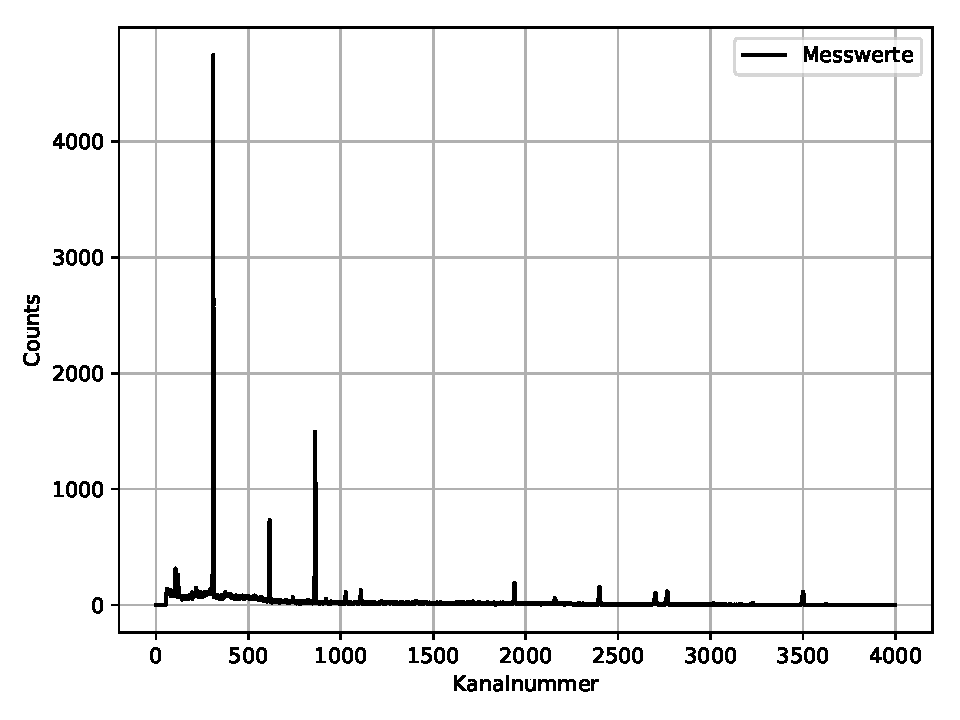
\includegraphics[height=9cm]{Eu.pdf}
  \caption{Spektrum des $\ce{^{152}Eu}$-Strahlers}
  \label{fig:plot1}
\end{figure}

Um mit diesem die Energiekalibration durchzuführen, werden die Peaks des Spektrums
jeweils mit einer Gaußverteilung der Form
\begin{equation}
  \symup{g} (x) = a + b \cdot \symup{e}^{(\frac{x-z}{c})^2}
  \label{eqn:gausk}
\end{equation}
gefittet.

Die sich daraus ergebenen Parameter sind in Tabelle \ref{tab:tabe1} angegebenen.
\begin{table}[H]
  \centering
  \caption{Messwerte der Wärmepumpe}
  \label{tab:tabe1}
    \begin{tabular}{S S S S S S}
    \toprule
    $ t  \: / \si{\second} $ & $ p_a \: / \si{\bar} $ & $ p_b \: / \si{\bar} $ &
    $ T_1 \: / \si{\kelvin} $ & $ T_2 \: / \si{\kelvin} $ & $ P \: / \: \si{\watt} $\\
    \midrule
    0 & 5.0 & 5.0 & 293.65 & 293.65 & 0 \\
    60 & 4.7 & 6.0 & 294.15 & 293.55 & 115 \\
    120 & 4.4 & 6.4 & 295.15 & 293.15 & 118 \\
    180 & 4.5 & 6.9 & 296.35 & 291.95 & 122 \\
    240 & 4.6 & 7.0 & 297.55 & 290.95 & 125 \\
    300 & 4.6 & 7.0 & 298.85 & 289.95 & 125 \\
    360 & 4.5 & 7.2 & 300.05 & 289.15 & 123 \\
    420 & 4.4 & 7.4 & 301.15 & 288.45 & 123 \\
    480 & 4.3 & 7.8 & 302.35 & 287.65 & 122 \\
    540 & 4.2 & 8.0 & 303.55 & 286.95 & 122 \\
    600 & 4.2 & 8.1 & 304.65 & 286.25 & 121 \\
    660 & 4.1 & 8.3 & 305.75 & 285.55 & 121 \\
    720 & 4.0 & 8.5 & 306.75 & 284.95 & 121 \\
    780 & 4.0 & 8.8 & 307.75 & 284.35 & 121 \\
    840 & 3.9 & 9.0 & 308.75 & 283.75 & 121 \\
    900 & 3.8 & 9.1 & 309.65 & 283.15 & 121 \\
    960 & 3.8 & 9.2 & 310.55 & 282.55 & 122 \\
    1020 & 3.8 & 9.5 & 311.45 & 282.05 & 122 \\
    1080 & 3.7 & 9.8 & 312.25 & 281.55 & 122 \\
    1140 & 3.7 & 10.0 & 313.05 & 281.15 & 122 \\
    1200 & 3.7 & 10.0 & 313.9 & 280.65 & 122 \\
    1260 & 3.6 & 10.2 & 314.65 & 280.25 & 123 \\
    1320 & 3.6 & 10.3 & 315.35 & 279.85 & 123 \\
    1380 & 3.6 & 10.6 & 316.15 & 279.45 & 124 \\
    1440 & 3.6 & 10.8 & 316.85 & 279.15 & 124 \\
    1500 & 3.6 & 11.0 & 317.55 & 278.75 & 124 \\
    1560 & 3.6 & 11.1 & 318.25 & 278.55 & 124 \\
    1620 & 3.6 & 11.2 & 318.95 & 278.25 & 125 \\
    1680 & 3.5 & 11.4 & 319.55 & 277.95 & 125 \\
    1740 & 3.5 & 11.5 & 320.15 & 277.65 & 125 \\
    1800 & 3.5 & 11.7 & 320.75 & 277.45 & 125 \\
    1860 & 3.5 & 11.9 & 321.35 & 277.25 & 125 \\
    1920 & 3.5 & 12.0 & 321.95 & 277.05 & 125 \\
    1980 & 3.5 & 12.1 & 322.45 & 276.95 & 125 \\








      \bottomrule
    \end{tabular}
\end{table}


Die zentrale Lage der Peaks im Hinblick auf die Kanalnummer ist durch den Parameter
z gegeben. Diese Werte werden zusammen mit der jeweiligen relativen Höhe mit den theoretischen
Emissionslinien der Datenbank \cite{lara} verglichen und es wird jedem Peak eine Linie
zugeordent. Diese Zuordnung ist zusammen mit der jeweiligen relativen Emissionswahrscheinlichkeit P
in Tabelle \ref{tab:tabe2} dargestellt.
\begin{table}[H]
  \centering
  \caption{Wertetabelle für $\alpha$ und $C_V$.}
  \label{tab:tab2}
    \begin{tabular}{S S S S S}
    \toprule
    $ T\: \text{in}\: \si{\K} $ & $ {\alpha \cdot 10^{-6} \: \text{in}\: \si {\per\K}} $ &
    $ C_V \: \text{in}\: \si{\J\per\K\mol} $\\
    \midrule %Cv, a *10-6, Cv
    %0 & 1 & 1\\
    88.60\pm0.24 & 9.56\pm0.06 & 14.17\pm8.13  \\ %&3.6 & 318.97\pm0.85\\
    93.81\pm0.24 & 10.10\pm0.06 & 17.58\pm10.03 \\ %& 4.7 & 440.90\pm1.11\\
    99.74\pm0.24 & 10.66\pm0.05 & 15.52\pm8.84 \\ %& 5.1 & 508.68\pm1.21\\
    104.74\pm0.24 & 11.07\pm0.05 & 18.44\pm10.52 \\ %& 4.6 & 481.79\pm1.09\\
    110.94\pm0.24 &  11.54\pm0.05 & 14.86\pm8.45 \\ %& 5.3 & 587.97\pm1.27\\
    115.96\pm0.24 & 11.89\pm0.05 & 18.49\pm10.52 \\ %& 4.6 & 533.41\pm1.10\\
    121.47\pm0.24 &  12.22\pm0.05 & 16.83\pm9.57 \\ %& 4.9 & 595.21\pm1.17\\
    126.99\pm0.24 & 12.53\pm0.04 & 16.79\pm9.54 \\ %& 4.9 & 622.29\pm1.18\\
    131.58\pm0.24 & 12.77\pm0.04 & 20.42\pm11.62 \\ %& 4.2 & 552.62\pm1.01\\
    136.65\pm0.24 & 13.02\pm0.04 & 18.40\pm10.47 \\ %& 4.6 & 628.57\pm1.11\\
    141.49\pm0.24 & 13.24\pm0.04 & 19.28\pm10.97 \\ %& 4.4 & 622.54\pm1.07\\
    146.34\pm0.24 & 13.44\pm0.04 & 19.24\pm10.95 \\ %& 4.4 & 643.88\pm1.07\\
    150.95\pm0.24 & 13.62\pm0.04 & 20.22\pm11.52 \\ %& 4.3 & 649.11\pm1.05\\
    155.34\pm0.24 & 13.79\pm0.04 & 21.31\pm12.14 \\ %& 4.1 & 636.88\pm0.98\\
    159.97\pm0.24 & 13.95\pm0.04 & 20.12\pm11.47 \\ %& 4.3 & 687.89\pm1.05\\
    164.62\pm0.24 & 14.10\pm0.04 & 20.18\pm11.51 \\ %& 4.3 & 707.87\pm1.06\\
    168.79\pm0.25 & 14.23\pm0.04 & 22.54\pm12.86 \\ %& 3.9 & 658.27\pm0.95\\
    173.45\pm0.25 &  14.37\pm0.04 & 20.08\pm11.46 \\ %& 4.3 & 745.84\pm1.06\\
    178.13\pm0.25 &  14.50\pm0.04 & 20.04\pm11.44 \\ %& 4.3 & 765.94\pm1.06\\
    182.56\pm0.25 &  14.62\pm0.04 & 21.11\pm12.06\\
    192.70\pm0.25 &  14.87\pm0.04 & 18.41\pm10.47\\
    200.15\pm0.25 &  15.04\pm0.04 & 25.19\pm14.28\\
    208.87\pm0.25 &  15.23\pm0.04 & 21.43\pm12.18\\
    217.12\pm0.25 &  15.38\pm0.04 & 22.65\pm12.88\\
    225.15\pm0.25 &  15.53\pm0.03 & 23.27\pm13.24\\
    232.70\pm0.25 &  15.70\pm0.03 & 24.75\pm14.08\\
    240.53\pm0.25 &  15.74\pm0.03 & 23.84\pm13.58\\
    248.39\pm0.25 &  15.89\pm0.03 & 23.74\pm13.53& \\
    256.01\pm0.25 &  15.97\pm0.03 & 24.46\pm13.94 \\
    263.41\pm0.26 &  16.01\pm0.03 & 25.22\pm14.38 \\
    271.08\pm0.26 &  16.18\pm0.03 & 24.26\pm13.86 \\
    278.52\pm0.26 &  16.27\pm0.03 & 25.03\pm14.29&\\
    285.98\pm0.26 &  16.35\pm0.03 & 24.92\pm14.25 \\
    293.21\pm0.26 &  16.42\pm0.03 & 25.74\pm14.72 \\
    300.98\pm0.26 &  16.50\pm0.03 & 23.87\pm13.68 \\
    308.51\pm0.26 &  16.57\pm0.03 & 24.63\pm14.12\\



      \bottomrule
    \end{tabular}
\end{table}

Mit den Wertepaaren aus Kanalnummer und Linienenergie wird nun eine lineare Ausgleichsrechnung der
Form
\begin{equation}
  f(x) = a\cdot x +b
  \label{eqn:li}
\end{equation}
durchgeführt, woraus sich die Parameter
\begin{align}
  a &= \SI{0.403169(29)}{\kilo\electronvolt} \\
  b &= \SI{-3.034(60)}{\kilo\electronvolt}
\end{align}
ergeben. Die Wertepaare sind zusammen mit der resultierenden Gerade in Abbildung \ref{fig:plot3}
dargestellt. Die Fehler der Messwerte sind aufgrund ihrer sehr geringen relativen Größe dabei zu vernachlässigen.
\begin{figure}
  \centering
  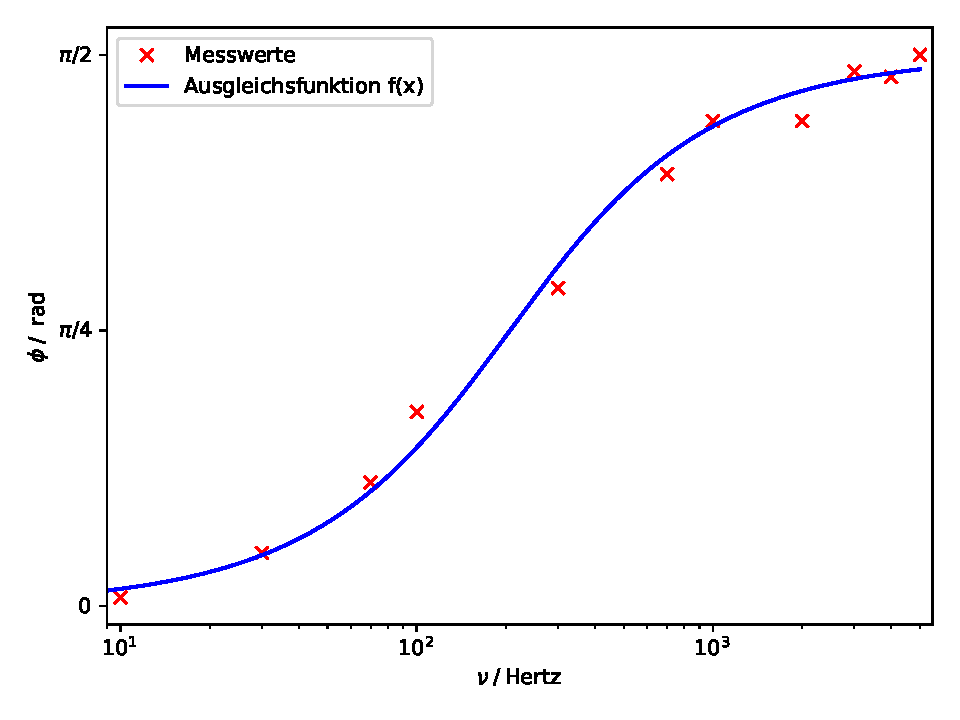
\includegraphics[height=9cm]{plot3.pdf}
  \caption{Lineare Ausgleichsrechnung zur Energiekalibration}
  \label{fig:plot3}
\end{figure}
Die Energiekalibration erfolgt somit gemäß
\begin{equation}
  \symup{E}_{\gamma} (x) = \SI{0.403169}{\kilo\electronvolt}\cdot x - \SI{3.034}{\kilo\electronvolt}
  \label{eqn:gerade}
\end{equation}
wobei x die Kanalnummer bezeichnet.
Der dazugehörige Fehler ergibt mittels Gleichung \ref{eqn:gaus} durch
\begin{equation}
   \increment \symup{E}_{\gamma} (x) =\sqrt{ (\SI{0.000029}{\kilo\electronvolt}\cdot x)^2 +
   (\SI{0.060}{\kilo\electronvolt})^2}
   \label{eqn:fgerade}
\end{equation}
\\
Zur Bestimmung der Vollenergienachweiswahrscheinlichkeit wird zunächst die Gleichung \ref{eqn:gausk}
integriert, um den Inhalt der Peaks zu bestimmen, wobei der Untegrund $a$ vorher abgezogen wird.
Es ergibt sich somit ein Linieninhalt von
\begin{equation}
  \symup{I} =\int_{-\infty}^{\infty} c \cdot \symup{e}^{(\frac{x-z}{b})^2} \symup{d}x
  = c \cdot b \cdot \sqrt{\pi}
  \label{eqn:inh}
\end{equation}
in Abhängigkeit der Parameter b und c.
Der Fehler ergibt sich durch Gleichung \ref{eqn:gaus} über die Gleichung
\begin{equation}
  \increment \symup{I} = \sqrt{ (\increment c \cdot b \cdot \sqrt{\pi})^{2}
   + (c \cdot \increment b \cdot \sqrt{\pi}})^{2} \: .
     \label{eqn:inhf}
\end{equation}
Mit den Werten aus Tabelle \ref{tab:tabe1} lassen sich somit die einzelnen Linieninhalte berrechen,
welche in Tabelle \ref{tab:tabe3} angegeben sind.
\begin{table}
  \centering
  \caption{Messwerte für den ersten Doppelspalt.}
   \begin{tabular}{S S| S S | S S}
    \toprule
    $x/\; \si{\mm}$& $A/\;\si{\nA}$ &
    $x/\; \si{\mm}$& $A/\;\si{\nA}$ &
    $x/\; \si{\mm}$& $A/\;\si{\nA}$ \\
    \midrule

    15.0& 4.6& 23.0& 25.0& 29.5& 6.0\\
    15.5& 4.2& 23.5& 30.0& 30.0& 5.3\\
    16.0& 4.0& 24.0& 35.0& 30.5& 4.9\\
    16.5& 4.0& 24.25& 36.0& 31.0& 4.7\\
    17.0& 4.4& 24.5& 37.0& 31.5& 4.4\\
    17.5& 5.5& 24.75& 38.0& 32.0& 4.2\\
    18.0& 6.6& 25.00& 37.0& 32.5& 3.8\\
    18.5& 7.7& 25.25& 36.0& 33.0& 3.6\\
    19.0& 8.2& 25.5& 36.0& 33.5& 3.2\\
    19.5& 8.4& 26.0& 33.0& 34.0& 3.2\\
    20.0& 8.4& 26.5& 28.5& 34.5& 3.2\\
    20.25& 8.4& 27.0& 23.0& 35.0& 3.3\\
    20.5& 8,7& 27.5& 18.0& 35.5& 3.4\\
    21.0& 9.8& 28.0& 13.5& 36.0& 3.5\\
    21.5& 12.0& 28.5& 10.0\\
    22.0& 15.0& 29.0& 7.8\\
    22.5& 20.0& 29.25& 6.7\\


   \bottomrule
  \end{tabular}
  \label{tab:tabelle3}
\end{table}

Zum Vergleich werden nun die Theoriewerte berrechnet, als Produkt
der Emissionswahrscheinlichkeiten P aus Tabelle \ref{tab:tabe2},
dem abgedeckten Raumwinkelanteil $\frac{\Omega}{4\pi}= 0.01558$, der errechneten Aktivität
$A =\SI{1599(29)}{\becquerel} $
und der Messzeit von $t = \SI{3598}{\second}$
\begin{equation}
  \symup{I}_{\text{theo}} = P\cdot \frac{\Omega}{4\pi} \cdot A \cdot t
  \label{eqn:itheo}
\end{equation}
mit dem Fehler über Gleichung \ref{eqn:gaus} von
\begin{equation}
  \increment \symup{I}_{\text{theo}} = \sqrt{ (\increment P\cdot \frac{\Omega}{4\pi} \cdot A \cdot t)^{2}
   + (P\cdot \frac{\Omega}{4\pi} \cdot \increment A \cdot t)^{2}} \: .
\end{equation}
Aus dem jeweiligen Quotienten
\begin{equation}
  \symup{Q} = \frac{\symup{I}}{\symup{I}_{\text{theo}}}
  \label{eqn:ven1}
\end{equation}
mit dem dazugehörigen Fehler
\begin{equation}
  \increment \symup{Q} = \sqrt{ (\frac{1}{\symup{I}_{\text{theo}} \cdot \increment \symup{I})^{2}
   + (\frac{\symup{I}}{\symup{I}_{\text{theo}}})^{2}}\cdot \increment \symup{I}_{\text{theo}})^{2}}
\end{equation}
ergibt sich somit jeweils die Nachweiswahrscheinlichkeit des Peaks, wie in Tabelle
\ref{tab:tabe4} dargestellt ist.
\begin{table}[H]
  \centering
   \begin{tabular}{c c c c}
    \toprule
    Nummer der Oberwelle & $ U_{\text Theorie,Rechteck}\: / \si{\volt} $ &
    $ U_{\text Theorie,Dreick}\: / \si{\volt} $ & $ U_{\text Theorie,Sägezahn}\: / \si{\volt} $ \\
    \midrule
    1 & 1145 & 182 & 573 \\
    2 & 0 & 0 & 286 \\
    3 & 573 & 20 & 191 \\
    4 & 0 & 0 & 143 \\
    5 & 229 & 7 & 115 \\
    6 & 0 & 0 & 96 \\
    7 & 164 & 4 & 82 \\
    8 & 0 & 0 & 72 \\
    9 & 127 & 2 & 64 \\
    10 & 0 & 0 & 57 \\
    \bottomrule
  \end{tabular}
  \caption{Eingestellte Schwingungsamplituden.}
  \label{tab:tabe4}
\end{table}

Da die Nachweiswahrscheinlichkeit im Allgemeinen energieabhängig ist, wird Q in
Abhängigkeit von $ \text{E}_{\gamma} $ dargestellt und mit einer Potenzfunktion der Form
\begin{equation}
  \symup{Q}(\text{E}_{\gamma}) = c\cdot (\text{E}_{\gamma}-a)^{d}
  \label{eqn:ven2}
\end{equation}
gefittet, wie in Abbildung \ref{fig:plot4} dargestellt ist.
Es ergeben sich hierbei die Parameter
\begin{align*}
  a &= -191 \pm 64 \\
  c &= 2474 \pm 3467 \\
  d &= -1.47 \pm 0.19 \: .
\end{align*}
 %Die Formel für die eigentliche Höhe eines
%gemessenen Peaks ergibt sich aus Gleichungen \ref{eqn:ven1} und \ref{eqn:ven2} durch Umstellen zu
%\begin{equation}
%  \symup{I}_{\text{theo}} = \frac{\symup{I}}{\symup{Q}}=\frac{\symup{I}}{c\cdot (\text{E}_{\gamma}-a)^{d}}
%  \label{eqn:ven}
%\end{equation}
%mit dem dazugehörigen Fehler
%\begin{equation}
%  \symup{I}_{\text{theo}} = \frac{\symup{I}}{\symup{Q}}=\frac{\symup{I}}{c\cdot (\text{E}_{\gamma}-a)^{d}}
%  NAMNAM
%  \label{eqn:ven}
%\end{equation}
\begin{figure}
  \centering
  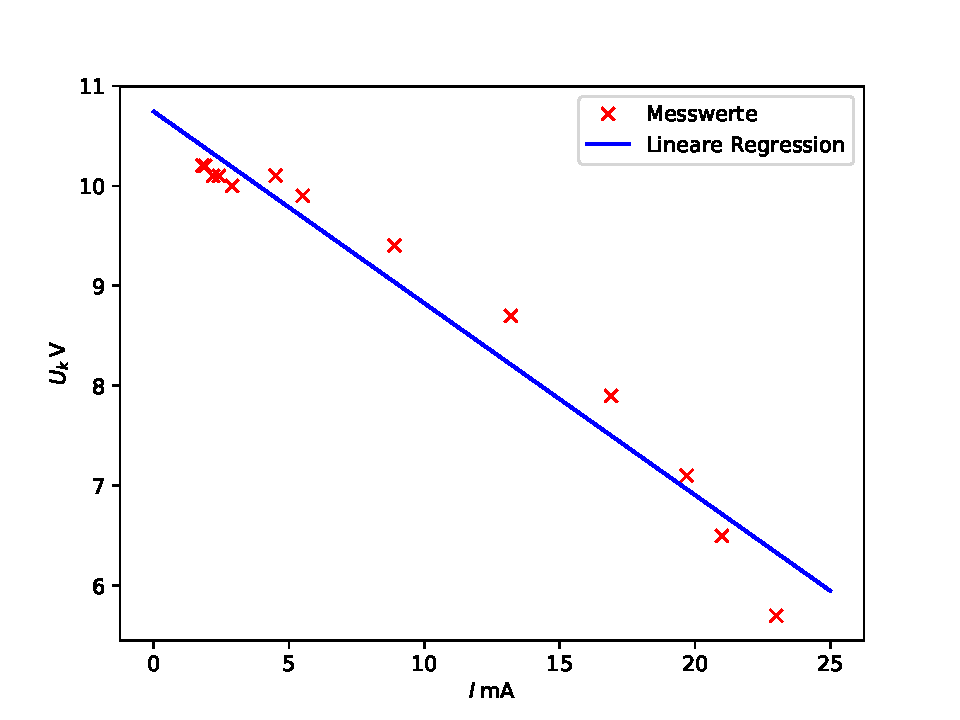
\includegraphics[height=9cm]{plot4.pdf}
  \caption{Werte zur Bestimmung der Vollenergienachweiswahrscheinlichkeit sowie gefittete Potenzfunktion}
  \label{fig:plot4}
\end{figure}

\subsection{Untersuchung eines monochromatischen Gamma-Spektrums}
Zur Untersuchung des monochromatischen Gamma-Spektrums wird das aufgenommene Spektrum
zunächst durch die Gleichung \ref{eqn:gerade} kalibriert, wobei sich der Fehler über
\ref{eqn:fgerade} ergibt. Die so erhaltenen Werte sind in Abbildung \ref{fig:plot5}
dargestellt, wobei auf Fehlerbalken aufgrund der geringen Fehler verzichtet wird. Die
Messzeit beträgt $\SI{2593}{\second}$ und es wurden 8191 Kanäle gemessen, wobei nur die
ersten 2000 dargestellt sind, da bei höheren Kanalnummern keine signifikanten Messwerte
mehr zu erkennen sind.
\begin{figure}
  \centering
  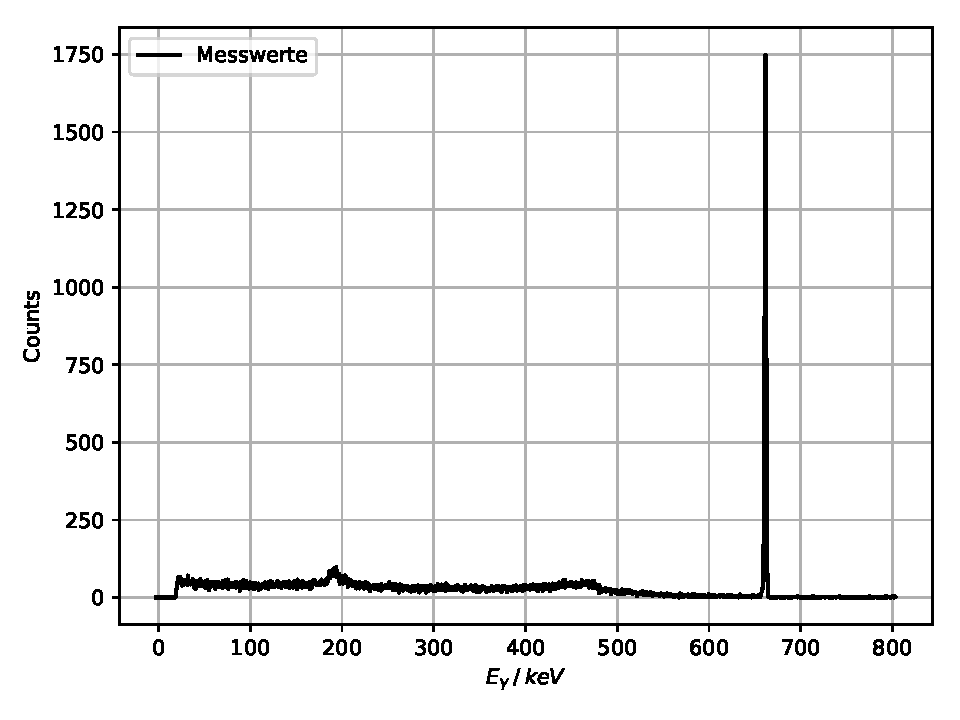
\includegraphics[height=9cm]{Cs.pdf}
  \caption{Kalibriertes Spektrum des $\ce{^{137}Cs}$-Strahlers }
  \label{fig:plot5}
\end{figure}
Zur Bestimmung der Energie wird die Vollenergielinie mit der Gaußverteilung aus Gleichung
\ref{eqn:gausk} gefittet, wobei sich die Parameter
\begin{align*}
  a &= 5.7 \pm 4.2 \\
  b &= 1674 \pm 17 \\
  c &= \SI{1.227(15)}{\kilo\electronvolt}\\
  z &= \SI{661.5985(98)}{\kilo\electronvolt} \:
\end{align*}
ergeben.
Die Energie des Strahlers ist dabei durch den Parameter $z$ gegeben, also
\begin{align*}
  \symup{E}_{Cs} = \SI{661.5985(98)}{\kilo\electronvolt} \: .
\end{align*}
Der Theoriewert von $\ce{^{137}Cs}$ beträgt $\SI{661.657(3)}{\kilo\electronvolt}$ \cite{lara}. \\
Der Bereich um die Vollenergielinie ist in
Abbildung \ref{fig:plot6} dargestellt, woraus sich die Halbwertsbreite und die
Zehntelwertsbreite ablesen lässt, wobei eine Ungenauigkeit durch
Ablesefehler von etwa $\SI{0.2}{\kilo\electronvolt}$ angenommen wird.
Es ergibt sich hierdurch
\begin{align*}
  \symup{E}_{1/2} = \SI{662.6(2)}{\kilo\electronvolt} -\SI{660.6(2)}{\kilo\electronvolt}
  =\SI{2.0(3)}{\kilo\electronvolt}\\
  \symup{E}_{1/10} = \SI{663.3(2)}{\kilo\electronvolt} -\SI{659.6(2)}{\kilo\electronvolt}
  =\SI{3.7(3)}{\kilo\electronvolt} \:
\end{align*}
woraus sich ein Verhältniss von
\begin{equation}
  \frac{\symup{E}_{1/2}}{\symup{E}_{1/10}} =  0.54 \pm 0.09 \:
\end{equation}
ergibt.
\begin{figure}
  \centering
  \includegraphics[height=9cm]{Plot6.pdf}
  \caption{Vollenergielinie}
  \label{fig:plot6}
\end{figure}
Die Halbwertsbreite einer Gaußkurve gemäß Gleichung \ref{eqn:gausk} ist durch die
Formel
\begin{equation}
  \symup{E}_{1/2} = 2c\cdot\sqrt{ln2}
\end{equation}
mit dem Fehler
\begin{equation}
  \increment \symup{E}_{1/2} = 2\increment b\cdot\sqrt{ln2} \: ,
\end{equation}
gegeben und beträgt somit
\begin{align*}
  \symup{E}_{1/2,theo} = \SI{1.701(21)}{\kilo\electronvolt} \: .
\end{align*}
Die Zehntelwertsbreite ergibt sich analog über die Gleichung
\begin{equation}
  \symup{E}_{1/10} = 2c\cdot\sqrt{ln10}
\end{equation}
mit dem Fehler
\begin{equation}
  \increment \symup{E}_{1/10} = 2\increment b\cdot\sqrt{ln10} \: ,
\end{equation}
zu
\begin{align*}
  \symup{E}_{1/10, theo} = \SI{5.651(69)}{\kilo\electronvolt} \: .
\end{align*}
Das Verhältniss dieser beiden Größen ist unabhängig von den jeweiligen Parametern der
Kurve stets
\begin{equation}
  \frac{\symup{E}_{1/2}}{\symup{E}_{1/10}} = \sqrt{\frac{ln2}{ln10}}
  \approx 0.549 \: ,
\end{equation}
Diese theoretisch erhaltenen Werte werden mit den abglesenen verglichen, wobei sich
die Abweichung über die Formel
\begin{equation}
  \frac{\lvert \text{Wert}_{\text{Theorie}}-\text{Wert}_{\text{Messung}}\rvert}{\text{Wert}_{\text{Theorie}}}
  \label{eqn:abw}
\end{equation}
berechnen lässt zu 1.64 \%. Diese Abweichung ist offensichtlich sehr gering und liegt innerhalb der
Ableseunsicherheit, was auf eine gute Beschreibung der Vollenergielinie
durch eine Gaußkurve schließen lässt. Die recht große Abweichung der Halb- und Zehntelwertsbreite
an sich lässt sich dadurch erklären, dass wohlmöglich eine falsche Maximalhöhe des Peaks angenommen
wurde.
Der Inhalt der Vollenergielinie ergibt sich durch Gleichungen \ref{eqn:inh}
und \ref{eqn:inhf} zu
\begin{align*}
  \symup{I}_{VEL} =  3641 \pm 58 \: .
\end{align*}
\\
Aus den Messwerten und Abbildung \ref{fig:plot5} lässt sich erkennen, dass die
Compton-Kante bei etwa $\SI{478(3)}{\kilo\electronvolt}$ liegt, da dort (Kanalnummer
1198) das Spektrum ein lokales
Maximum von 53 Counts animmt und anschließend abfällt, wobei die Ableseunsicherheit auf etwa
$\SI{3}{\kilo\electronvolt}$ geschätzt wird.
Aus Gleichung \ref{eqn:kante} ergibt sich der theoretische Wert zu $\SI{477.280(90)}{\kilo\electronvolt}$
und die Abweichung somit zu 0.15 \%.
Um den Inhalt des Comptonkontinuums zu bestimmen wird der Bereich zwischen $\SI{20}{\kilo\electronvolt}$
und $\SI{478}{\kilo\electronvolt}$ mit der Funktion aus Gleichung \ref{eqn:diffCompton} gefittet,
wobei der Term $a =\frac{3}{8}\sigma_{\text{Th}}\frac{1}{m_0 c^2 e^2}$ als Fitparameter
verwendet wird. Für diesen ergibt sich
\begin{align*}
  a =  4.297 \pm 0.056 \: .
\end{align*}
Dieser Wert wird nun verwendet, um die Funktion numerisch in dem Bereich zwischen $\SI{20}{\kilo\electronvolt}$
und $\SI{478}{\kilo\electronvolt}$
zu integrieren, wodurch sich der Inhalt des Comptonkontinuums zu
\begin{align*}
  \symup{I}_{Compton} =  16266 \pm 214
\end{align*}
ergibt.

Der Rückstreupeak wird erneut mit der Gleichung \ref{eqn:gausk} gefittet, wodurch sich
die Parameter
\begin{align*}
  a &= 65.8 \pm 2.0 \\
  b &= 36 \pm 28 \\
  c &= \SI{0.28(28)}{\kilo\electronvolt}\\
  z &= \SI{193.78(24)}{\kilo\electronvolt} \:
\end{align*}
ergeben, der Rückstreupeak liegt also bei $\SI{193.78(24)}{\kilo\electronvolt}$.
Der Theoriewert nach Gleichung \ref{eqn:Rückstreu} ergibt sich zu $\SI{184.3184(76)}{\kilo\electronvolt}$.
\\
Zur Bestimmung der Absorptionswahrscheinlichkeiten wird die Formel
\begin{equation}
  \symup{p} = 1-\exp{-\mu \cdot l}
\end{equation}
verwendet, wobei $l$ die Länge des Detektors, in diesem Fall also $\SI{3.9}{\centi\meter}$, bezeichnet
und $\mu$ den Extinkionskoeffizient, welcher für den Comptoneffekt etwa
$\mu_{c}=\SI{0.38}{\per\centi\meter}$ und für den Photoeffekt etwa
$\mu_{p}=\SI{0.008}{\per\centi\meter}$ beträgt.
Dies führt zu Absorptionswahrscheinlicheiten von
\begin{align*}
  \symup{p}_{c} = 0.7728 \\
  \symup{p}_{p} = 0.0307 \: ,
\end{align*}
sodass sich theoretisch ein Verhältniss zwischen den Inhalten des Photopeaks und des
Comptonkontinuums von
\begin{equation*}
  (\frac{\symup{I}_{VEL}}{\symup{I}_{Compton}})_{\text{theo}} = 1-\symup{e}{-\mu \cdot l}
  = 0.03975
\end{equation*}
ergeben sollte. Das tatsächliche Verhältniss aus den Messdaten beträgt
\begin{equation*}
  \frac{\symup{I}_{VEL}}{\symup{I}_{Compton}}
  = 0.224 \pm 0.005
\end{equation*}
und weist somit eine Abweichung von 463.52 \% auf, gemäß Formel \ref{eqn:abw}.


\subsection{Aktivitätsbestimmung}
Bei dem dritten vermessenen Spektrum soll zunächst festgestellt werden, ob es sich bei der gemessenen
Probe um einen $\ce{^{133}Ba}$-Strahler oder einen $\ce{^{125}Sb}$-Strahler handelt. Zu diesem
Zweck wird das Spektrum zunächst gemäß Gleichung \ref{eqn:gerade} kalibriert, wie in Abbildung
\ref{fig:plot7} dargestellt ist. Die Messzeit beträgt $\SI{4378}{\second}$; von den 8191 verwendeten
Kanälen werden nur die ersten 2000 verwendet, da darüber hinaus keine signifikanten
Messwerte mehr zu erkennen sind.
\begin{figure}
  \centering
  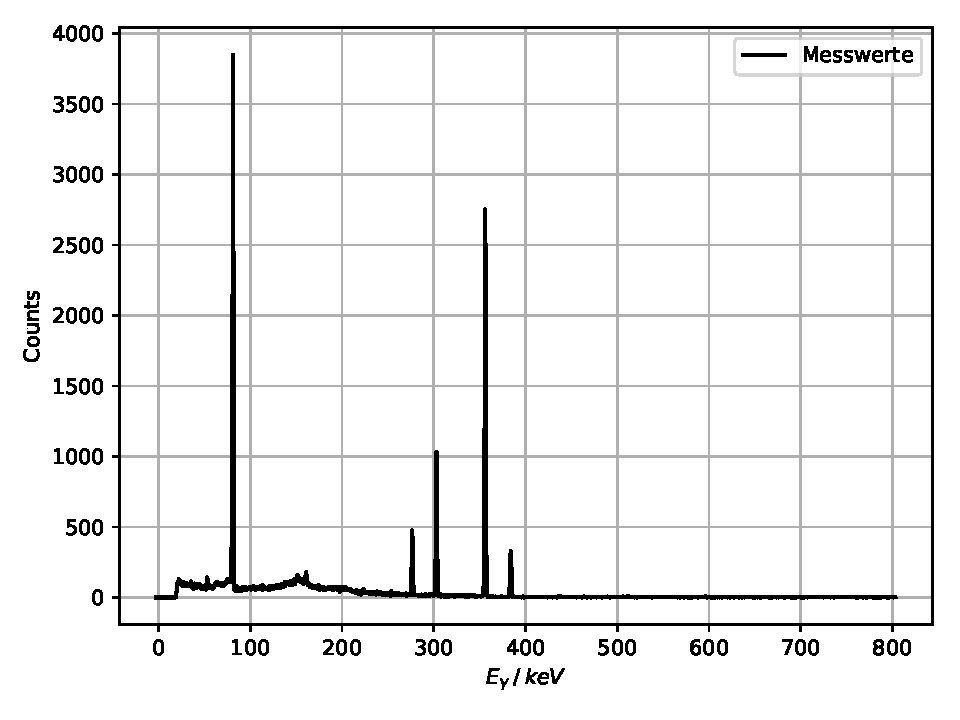
\includegraphics[height=9cm]{Ba.pdf}
  \caption{Unbekanntes Spektrum}
  \label{fig:plot7}
\end{figure}
Die Peaks werden erneut mit Gleichung \ref{eqn:gausk} gefittet und die resultierenden
Parameter in Tabelle \ref{tab:tabe5} dargestellt.
\begin{table}[H]
  \centering
  \caption{Bohrung 1 und 2, Vergleich der Sonden mit 1\;MHz und 2\;MHz.}
  \label{tab:tab5}
    \begin{tabular}{c c c c}
    \toprule
    Bohrung & $S_{\text{2\;MHz}}$/\;mm & $S_{\text{ 1\;MHz}}$/\;mm\\
    \midrule
    1 & 1,82 & 2,12\\
    2 & 1,83 & 1,97\\
    \bottomrule
    \end{tabular}
  \end{table}

Durch einen Vergleich mit der Datenbank
\cite{Lara} fällt auf, dass die Peaks mit denen von Barium übereinstimmen und es sich somit
bei der Probe offensichtlich um Barium handelt. Die Zuordnung zu den theoretischen Emissionslinien
und die entsprechenden Absorptionswahrscheinlickeiten sind in Tabelle \ref{tab:tabe6} angegeben.
\begin{table}[H]
  \centering
  \caption{Werte der Anpassungsschicht}
  \label{tab:tabe6}
    \begin{tabular}{S S S }
    \toprule
    $ \text{Zylinder} $ & $ \increment t [\mu\text{s}] $ &
    $ l_a \text{[mm]}$\\
    \midrule
    1 & 0.54 & 0.81 \\
    2 & 0.40 & 0.59 \\
    3 & 0.76 & 1.12 \\
    \text{1+2} & 0.49 & 0.73 \\
    4 & 0.70 & 1.03 \\
    \text{1+3} & 0.90 & 1.33 \\
    5 & 1.25 & 1.85 \\
    \text{1+4} & 0.69 & 1.02 \\
    6 & 0.44 & 0.66 \\

          \bottomrule
    \end{tabular}
  \end{table}

Zur Bestimmung der Aktivität wird mittels Gleichung \ref{eqn:inh} zunächst der Inhalt der Peaks errechnet.
Aus Gleichung \ref{eqn:itheo} lässt sich ein linearer Zusammenhang zwischen diesem Inhalt und der Aktivität
erkennen, wobei der Proportionalitätsfaktor durch
\begin{equation}
  l = P\cdot \frac{\Omega}{4\pi}\cdot t \cdot Q
  \label{eqn:lin}
\end{equation}
gegeben ist. Zur Bestimmung der Aktivität wird also eine Lineare Ausgleichsrechnung
gemäß Formel \ref{eqn:li} mit Wertepaaren aus $l$ und $\symup{I}$ durchgeführt,
wobei der Fitparameter a die Aktivität angibt. Dabei wird die $\SI{81.0657}{\kilo\electronvolt}$
außer Acht gelassen, da bei so niedrigen Energien der Quotient $Q$ der Vollenergienachweiswahrscheinlichkeit
zu ungenau ist. Somit ergeben sich die Parameter
\begin{align*}
  a = 416.4 \pm 2.7 \\
  b = 35 \pm 14
\end{align*}
und damit eine Aktivität von $\SI{416.4(27)}{\becquerel} $.
Die Wertepaare und die Ausgleichsgerade sind in Abbildung \ref{fig:plot9} dargestellt.
\begin{figure}
  \centering
  \includegraphics[height=9cm]{Plot9.pdf}
  \caption{Lineare Regression zur Aktivitätsbestimmung von $\ce{^{133}Ba}$}
  \label{fig:plot9}
\end{figure}



\subsection{Nuklididentikation}
Im letzten Versuchsteil wird eine Probe unbekannter Zusammensetzung untersucht, wobei die
Messzeit $\SI{4064}{\second}$ beträgt. Von den 8191 gemessenen Kanälen werden die ersten 6000 zur Auswertung
verwendet, die entsprechenden Messwerte werden gemäß Gleichung \ref{eqn:gerade} kalibriert und
sind in Abbildung \ref{fig:plot8} dargestellt.
\begin{figure}
  \centering
  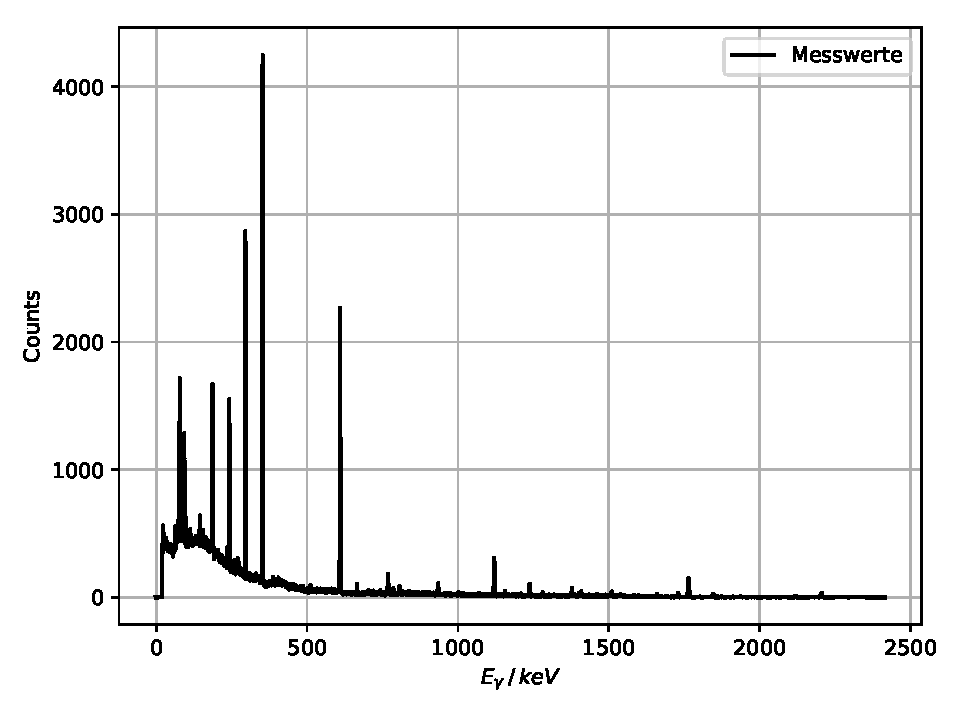
\includegraphics[height=9cm]{Un.pdf}
  \caption{Unbekanntes Spektrum}
  \label{fig:plot8}
\end{figure}

Um die Energie der Peaks zu bestimmen und sie somit zuordnen zu können, werden sie
wieder an die Gaußkurve gemäß Gleichung \ref{eqn:gausk} angepasst. Die Fitparameter sind in Tabelle
\ref{tab:tabe7} angegeben.

\begin{table}[H]
  \centering
  \caption{Parameter der gefitteten Gaußkurven}
  \label{tab:tabe7}
    \begin{tabular}{l l l l}
    \toprule
    $ a $ & $ b $ & $ c $
    & $ z \:/ \:\si{\kilo\electronvolt} $ \\
    \midrule
    593 \pm 23 & 1156 \pm 143 & 0.573 \pm 0.083 & 77.124 \pm 0.058 \\
    556 \pm 17 & 769 \pm 104 & 0.603 \pm 0.095 & 92.632 \pm 0.066 \\
    375.6 \pm 4.9 & 1335 \pm 25 & 0.772 \pm 0.017 & 186.090 \pm 0.012 \\
    252.8 \pm 6.2 & 1308 \pm 33 & 0.719 \pm 0.022 & 242.066 \pm 0.015 \\
    179.7 \pm 2.7 & 2711 \pm 14 & 0.7850 \pm 0.0048 & 295.3181 \pm 0.0033 \\
    130.2 \pm 4.2 & 4164 \pm 21 & 0.8586 \pm 0.0050 & 352.0054 \pm 0.0034 \\
    46.7 \pm 3.0 & 2230 \pm 12 & 1.1737 \pm 0.0076 & 609.2939 \pm 0.0052 \\
    31.3 \pm 1.1 & 64.9 \pm 4.2 & 1.33 \pm 0.10 & 665.409 \pm 0.070 \\
    31.3 \pm 1.3 & 158.5 \pm 4.6 & 1.451 \pm 0.051 & 768.246 \pm 0.034 \\
    30.9 \pm 1.0 & 38.9 \pm 3.9 & 1.29 \pm 0.16 & 785.87 \pm 0.10 \\
    30.7 \pm 1.0 & 46.6 \pm 4.1 & 1.20 \pm 0.13 & 806.244 \pm 0.085 \\
    26.3 \pm 1.1 & 72.9 \pm 3.7 & 1.68 \pm 0.10 & 934.015 \pm 0.067 \\
    18.2 \pm 1.9 & 292.3 \pm 5.8 & 1.782 \pm 0.043 & 1120.275 \pm 0.028 \\
    16.44 \pm 0.76 & 32.8 \pm 2.3 & 1.87 \pm 0.16  & 1155.44 \pm 0.10 \\
    13.1 \pm 1.1 & 98.2 \pm 3.1 & 2.037 \pm 0.078 & 1238.098 \pm 0.051 \\
    16.17 \pm 0.93 & 55.9 \pm 2.7 & 1.91 \pm 0.11 & 1377.862 \pm 0.074 \\
    17.5 \pm 1.3 & 25.6 \pm 3.8 & 1.95 \pm 0.36 & 1408.31 \pm 0.23 \\
    13.89 \pm 0.95 & 19.6 \pm 2.4 & 2.33 \pm 0.36 & 1509.44 \pm 0.22 \\
    4.78 \pm 0.63 & 12.2 \pm 1.3 & 2.96 \pm 0.40 & 1661.07 \pm 0.24 \\
    3.029 \pm 0.73 & 28.2 \pm 1.6 & 2.75 \pm 0.20 & 1729.76 \pm 0.12 \\
    3.0 \pm 1.79 & 145.9 \pm 3.9 & 2.725 \pm 0.093 & 1764.689 \pm 0.057 \\
    3.56 \pm 0.78 & 20.2 \pm 1.7 & 2.77 \pm 0.29 & 1847.40 \pm 0.18 \\
    0.71 \pm 0.87 & 29.1 \pm 1.6 & 3.35 \pm 0.24 & 2204.71 \pm 0.13 \\



          \bottomrule

    \end{tabular}
\end{table}

Die Linienenergien werden dann mit der Datenbank \cite{lara} abgeglichen und
passenden Nukliden zugeordent.
Diese Zuordnung ist in Tabelle \ref{tab:tabe8} zusammen mit den jeweiligen Emissionswahrscheinlichkeiten
dargestellt.
\begin{table}[H]
  \centering
  \caption{Werte der Messreihe die Wien-Robinson-brücke}
  \label{tab:tabe8}
    \begin{tabular}{c c c c}
    \toprule
    $ \nu \: / \: \si{\hertz} $ & $\text{U}_b \: / \: \si{\volt} $ &
    $\text{U}_s \: / \: \si{\volt} $ &
    $\frac{U_b}{U_s}$ \\
    \midrule
    20 & 0.120 & 3.08 & 0.039 \\
    50 & 0.248 & 4.56 & 0.054 \\
    100 & 0.320 & 4.64 & 0.069 \\
    150 & 0.264 & 4.56 & 0.058 \\
    200 & 0.136 & 4.50 & 0.030 \\
    220 & 0.072 & 4.48 & 0.016 \\
    230 & 0.032 & 4.48 & 0.007 \\
    240 & 0.024 & 4.48 & 0.005 \\
    242 & 0.016 & 4.48 & 0.004 \\
    250 & 0.040 & 4.48 & 0.009 \\
    265 & 0.080 & 4.48 & 0.018 \\
    300 & 0.298 & 4.56 & 0.065 \\
    500 & 0.704 & 4.56 & 0.154 \\
    1000 & 1.17 & 4.32 & 0.271 \\
    3000 & 1.41 & 4.28 & 0.330 \\
    10000 & 1.44 & 4.24 & 0.340 \\
    20000 & 1.44 & 4.24 & 0.340 \\
    30000 & 1.44 & 4.24 & 0.340 \\

    \bottomrule
    \end{tabular}
\end{table}

Alle identifizierten Nuklide gehören zu der Uran-Radium Zerfallsreihe, welche auch als 4n+2
Reihe bekannt ist. Es lässt sich also vermuten, dass die Probe ursprünglich zum Teil aus
$\ce{^{238}U}$ oder $\ce{^{234}Th}$ bestand, welches über  die Zeit zerfallen ist und somit die
radioaktiven Tochternuklide $\ce{^{226}Ra}$, $\ce{^{214}Pb}$ und $\ce{^{214}Bi}$ erklärt.
Alle weiteren Nuklide der Reihe haben keine, oder zumindest nur sehr schwache
Gammasignaturen, sodass diese nicht detektiert werden können.
Für die Aktivitätsbestimmung sind nur bei $\ce{^{214}Pb}$ und $\ce{^{214}Bi}$ genügend
Linien vorhanden um eine nicht allzu ungenaue Rechnung durchführen zu können. Das Vorgehen ist analog zur
Bestimmung der Aktivität von $\ce{^{133}Ba}$ und die resultierenden Ausgleichsgeraden sind in den
Abbildungen \ref{fig:plot11} und \ref{fig:plot12} dargestellt. Bei der Aktivitätsbestimmung
von $\ce{^{214}Pb}$ wurde die $\SI{77.1088}{\kilo\electronvolt}$ Linie außer acht gelassen,
da hier der Quotient $Q$ zu ungenau ist.
Es ergeben sich die Fitparameter
\begin{align*}
  a_{\text{Pb}} &= 1106 \pm 17 \\
  b_{\text{Pb}} &= -6\pm 69 \\
  a_{\text{Bi}} &= 1442 \pm 89 \\
  b_{\text{Bi}} &= 7 \pm 21 \\
\end{align*}
und somit Aktivitäten von $\SI{1106(17)}{\becquerel} $ für $\ce{^{214}Pb}$ und
$\SI{1442(89)}{\becquerel} $ für $\ce{^{214}Bi}$.
\begin{figure}
  \centering
  \includegraphics[height=9cm]{Plot11.pdf}
  \caption{Lineare Regression zur Aktivitätsbestimmung von $\ce{^{214}Pb}$}
  \label{fig:plot11}
\end{figure}
\begin{figure}
  \centering
  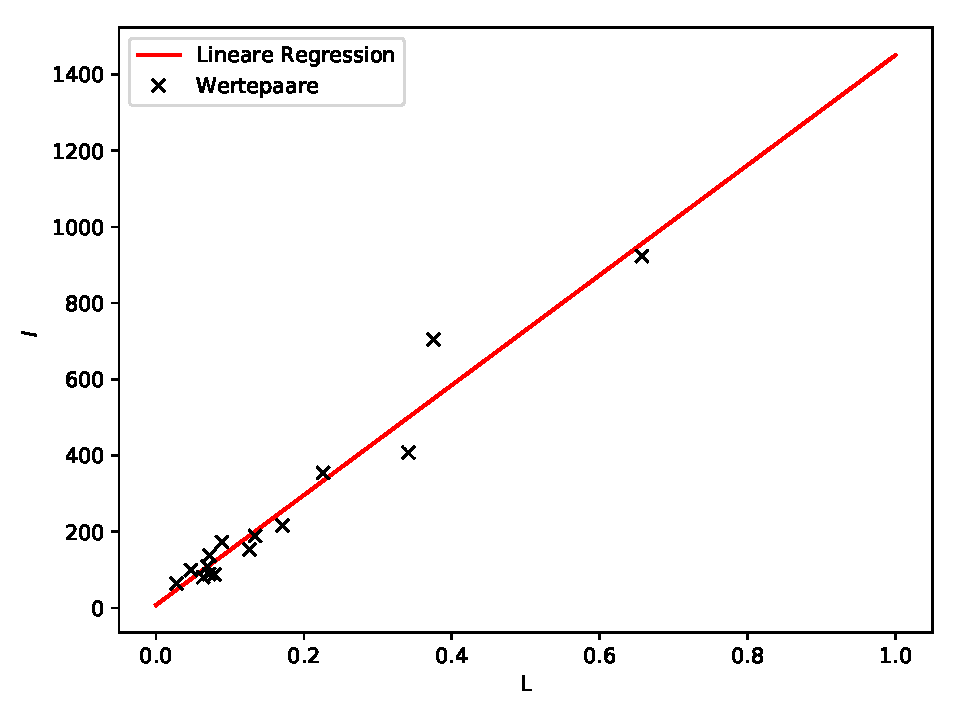
\includegraphics[height=9cm]{plot12.pdf}
  \caption{Lineare Regression zur Aktivitätsbestimmung von $\ce{^{214}Bi}$}
  \label{fig:plot12}
\end{figure}

\section{Diskussion}
Die lineare Regression zur Bestimmung der Energiekalibration liefert sehr geringe Ungenauigkeiten
der Fitparameter und scheint somit sehr exakt zu sein, was für ein gutes Auflösungsvermögen
des Detektors spricht. Die Parameter des Fits für die Vollenergienachweiswahrscheinlichkeit sind hingegen
mit einem großen relativen Fehler behaftet, welche teilweise sogar größer als der
eigentliche Wert sind. Dies lässt darauf schließen, dass eine Potenzfunktion
nicht vollständig zur Beschreibung der Energieabhängigkeit geeignet ist und
eine andere Funktion eventuell besser zu den Daten passen würde. \\
Die Abweichung in der gemessenen Energie des $\ce{^{137}Cs}$-Strahlers beträgt lediglich
0.0088\%, wodurch erneut die gute Energieauflösung gezeigt wird. Wie bereits erwähnt
ist die Beschreibung der Peaks durch Gaußkurve sehr genau und weißt im Verhältniss
von Halb- und Zehntelwertsbreite nur eine Abweichung von 1.64 \% auf. \\
Auch die Componkante und das Comptonkontinuum können recht genau bestimmt werden,
jedoch ergibt sich bei dem Rückstreupeak eine Abweichung von 5,14 \% , wobei der Theoriewert etwa 39,44
Fehlerintervalle von dem experimentellen Wert abweicht. Es wird somit vermutlich ein systematischer Fehler
vorliegen. \\
Auch bei dem Verhältniss des Inhalts von Comptonkontinuum und Photopeak gibt es eine
sehr große Abweichung, was vermutlich daran liegt, dass Mehrfachstreuung beim
Comptoneffekt in den theoretischen Formeln nicht berücksichtigt wird. Durch diese
Mehrfachstreuung deponiert die Gammastrahlung einen größeren Anteil oder eventuell auch die
gesamte Energie in dem Detektor, sodass der Inhalt des Comptonkontinuums sinkt und der
Inhalt des Photopeaks steigt, was den Betrag des Verhältnisses ansteigen lässt. \\
Die Aktivität lässt sich ebenfalls bis auf einen geringen
relativen Fehler bestimmen und auch die Zuordnung der Proben ist aufgrund der
guten Energieauflösung problemlos möglich. Lediglich die $\SI{92.38(1)}{\kilo\electronvolt}$-Linie
und die $\SI{92.80(1)}{\kilo\electronvolt}$-Linie von $\ce{^{234}Th}$ können nicht
getrennt aufgelöst werden, sondern erscheinen als ein einzelner Peak. Hier liegt offensichtlich
die Grenze des Auflösungsvermögens.


\printbibliography{}

\end{document}
>>>>>>> michelson
